% ******************************* PhD Thesis Template **************************
% Please have a look at the README.md file for info on how to use the template

\documentclass[a4paper,12pt,numbered,print,index,oneside]{classes/PhDThesisPSnPDF}

% ******************************************************************************
% ******************************* Class Options ********************************
% *********************** See README for more details **************************
% ******************************************************************************

% `a4paper'(The University of Cambridge PhD thesis guidelines recommends a page
% size a4 - default option) or `a5paper': A5 Paper size is also allowed as per
% the Cambridge University Engineering Deparment guidelines for PhD thesis
%
% `11pt' or `12pt'(default): Font Size 10pt is NOT recommended by the University
% guidelines
%
% `oneside' or `twoside'(default): Printing double side (twoside) or single
% side.
%
% `print': Use `print' for print version with appropriate margins and page
% layout. Leaving the options field blank will activate Online version.
%
% `index': For index at the end of the thesis
%
% `draftclassic': For draft mode without loading any images (same as draft in book)
%
% `draft': Special draft mode with line numbers, images, and water mark with
% timestamp and custom text. Position of the text can also be modified.
%
% `abstract': To generate only the title page and abstract page with
% dissertation title and name, to submit to the Student Registry
%
% `chapter`: This option enables only the specified chapter and it's references
%  Useful for review and corrections.
%
% ************************* Custom Page Margins ********************************
%
% `custommargin`: Use `custommargin' in options to activate custom page margins,
% which can be defined in the preamble.tex. Custom margin will override
% print/online margin setup.
%
% *********************** Choosing the Fonts in Class Options ******************
%
% `times' : Times font with math support. (The Cambridge University guidelines
% recommend using times)
%
% `fourier': Utopia Font with Fourier Math font (Font has to be installed)
%            It's a free font.
%
% `customfont': Use `customfont' option in the document class and load the
% package in the preamble.tex
%
% default or leave empty: `Latin Modern' font will be loaded.
%
% ********************** Choosing the Bibliography style ***********************
%
% `authoryear': For author-year citation eg., Krishna (2013)
%
% `numbered': (Default Option) For numbered and sorted citation e.g., [1,5,2]
%
% `custombib': Define your own bibliography style in the `preamble.tex' file.
%              `\RequirePackage[square, sort, numbers, authoryear]{natbib}'.
%              This can be also used to load biblatex instead of natbib
%              (See Preamble)
%
% **************************** Choosing the Page Style *************************
%
% `default (leave empty)': For Page Numbers in Header (Left Even, Right Odd) and
% Chapter Name in Header (Right Even) and Section Name (Left Odd). Blank Footer.
%
% `PageStyleI': Chapter Name next & Page Number on Even Side (Left Even).
% Section Name & Page Number in Header on Odd Side (Right Odd). Footer is empty.
%
% `PageStyleII': Chapter Name on Even Side (Left Even) in Header. Section Number
% and Section Name in Header on Odd Side (Right Odd). Page numbering in footer

% Uncomment to change page style
% \pagestyle{PageStyleII}


% ********************************** Preamble **********************************
% Preamble: Contains packages and user-defined commands and settings
% ******************************************************************************
% ****************************** Custom Margin *********************************

% Add `custommargin' in the document class options to use this section
% Set {innerside margin / outerside margin / topmargin / bottom margin}  and
% other page dimensions
\ifsetCustomMargin
  \RequirePackage[left=37mm,right=30mm,top=35mm,bottom=30mm]{geometry}
  \setFancyHdr % To apply fancy header after geometry package is loaded
\fi

% Add spaces between paragraphs
\setlength{\parskip}{0.5em}
% Ragged bottom avoids extra whitespaces between paragraphs
\raggedbottom
% To remove the excess top spacing for enumeration, list and description
%\usepackage{enumitem}
%\setlist[enumerate,itemize,description]{topsep=0em}

% *****************************************************************************
% ******************* Fonts (like different typewriter fonts etc.)*************

% Add `customfont' in the document class option to use this section

\ifsetCustomFont
  % Set your custom font here and use `customfont' in options. Leave empty to
  % load computer modern font (default LaTeX font).
  %\RequirePackage{helvet}

  % For use with XeLaTeX
  %  \setmainfont[
  %    Path              = ./libertine/opentype/,
  %    Extension         = .otf,
  %    UprightFont = LinLibertine_R,
  %    BoldFont = LinLibertine_RZ, % Linux Libertine O Regular Semibold
  %    ItalicFont = LinLibertine_RI,
  %    BoldItalicFont = LinLibertine_RZI, % Linux Libertine O Regular Semibold Italic
  %  ]
  %  {libertine}
  %  % load font from system font
  %  \newfontfamily\libertinesystemfont{Linux Libertine O}
\fi

% *****************************************************************************
% **************************** Custom Packages ********************************

% ************************* Algorithms and Pseudocode **************************

%\usepackage{algpseudocode}


% ********************Captions and Hyperreferencing / URL **********************

% Captions: This makes captions of figures use a boldfaced small font.
%\RequirePackage[small,bf]{caption}

\RequirePackage[labelsep=space,tableposition=top]{caption}
\renewcommand{\figurename}{Fig.} %to support older versions of captions.sty


% *************************** Graphics and figures *****************************

%\usepackage{rotating}
\usepackage{wrapfig}
\usepackage[export]{adjustbox}

% Uncomment the following two lines to force Latex to place the figure.
% Use [H] when including graphics. Note 'H' instead of 'h'
%\usepackage{float}
%\restylefloat{figure}

% Subcaption package is also available in the sty folder you can use that by
% uncommenting the following line
% This is for people stuck with older versions of texlive
%\usepackage{sty/caption/subcaption}
\usepackage{subcaption}

% ********************************** Tables ************************************
\usepackage{booktabs} % For professional looking tables
\usepackage{multirow}

%\usepackage{multicol}
%\usepackage{longtable}
%\usepackage{tabularx}


% *********************************** SI Units *********************************
% \usepackage{siunitx} % use this package module for SI units


% ******************************* Line Spacing *********************************

% Choose linespacing as appropriate. Default is one-half line spacing as per the
% University guidelines

\doublespacing
% \onehalfspacing
% \singlespacing


% ************************ Formatting / Footnote *******************************

% Don't break enumeration (etc.) across pages in an ugly manner (default 10000)
%\clubpenalty=500
%\widowpenalty=500

%\usepackage[perpage]{footmisc} %Range of footnote options


% *****************************************************************************
% *************************** Bibliography  and References ********************

%\usepackage{cleveref} %Referencing without need to explicitly state fig /table

% Add `custombib' in the document class option to use this section
\ifuseCustomBib
   \RequirePackage[square, sort, numbers, authoryear]{natbib} % CustomBib

% If you would like to use biblatex for your reference management, as opposed to the default `natbibpackage` pass the option `custombib` in the document class. Comment out the previous line to make sure you don't load the natbib package. Uncomment the following lines and specify the location of references.bib file

%\RequirePackage[backend=biber, style=numeric-comp, citestyle=numeric, sorting=nty, natbib=true]{biblatex}
%\addbibresource{References/references} %Location of references.bib only for biblatex, Do not omit the .bib extension from the filename.

\fi

% changes the default name `Bibliography` -> `References'
\renewcommand{\bibname}{References}


% ******************************************************************************
% ************************* User Defined Commands ******************************
% ******************************************************************************

% *********** To change the name of Table of Contents / LOF and LOT ************

%\renewcommand{\contentsname}{My Table of Contents}
%\renewcommand{\listfigurename}{My List of Figures}
%\renewcommand{\listtablename}{My List of Tables}


% ********************** TOC depth and numbering depth *************************

\setcounter{secnumdepth}{2}
\setcounter{tocdepth}{2}


% ******************************* Nomenclature *********************************

% To change the name of the Nomenclature section, uncomment the following line

%\renewcommand{\nomname}{Symbols}


% ********************************* Appendix ***********************************

% The default value of both \appendixtocname and \appendixpagename is `Appendices'. These names can all be changed via:

%\renewcommand{\appendixtocname}{List of appendices}
%\renewcommand{\appendixname}{Appndx}

% *********************** Configure Draft Mode **********************************

% Uncomment to disable figures in `draft'
%\setkeys{Gin}{draft=true}  % set draft to false to enable figures in `draft'

% These options are active only during the draft mode
% Default text is "Draft"
%\SetDraftText{DRAFT}

% Default Watermark location is top. Location (top/bottom)
%\SetDraftWMPosition{bottom}

% Draft Version - default is v1.0
%\SetDraftVersion{v1.1}

% Draft Text grayscale value (should be between 0-black and 1-white)
% Default value is 0.75
%\SetDraftGrayScale{0.8}


% ******************************** Todo Notes **********************************
%% Uncomment the following lines to have todonotes.

%\ifsetDraft
%	\usepackage[colorinlistoftodos]{todonotes}
%	\newcommand{\mynote}[1]{\todo[author=kks32,size=\small,inline,color=green!40]{#1}}
%\else
%	\newcommand{\mynote}[1]{}
%	\newcommand{\listoftodos}{}
%\fi

% Example todo: \mynote{Hey! I have a note}

% *****************************************************************************
% ******************* Better enumeration my MB*************
\usepackage{enumitem}

\usepackage{courier}
\usepackage{tikz}
\usepackage{pgfplots}
\pgfplotsset{compat=newest}
\usetikzlibrary{plotmarks}
\usetikzlibrary{arrows.meta}
\usepgfplotslibrary{patchplots}
\usepackage{grffile}
\usepackage{amsmath}
\usepackage{epigraph}

\newcommand{\networkLayer}[6]{
\def\a{#1} % Used to distinguish input resolution for current layer.
\def\b{0.03}
\def\c{#2} % Width of the cube to distinguish number of input channels for current layer.
\def\t{#3} % X offset for current layer.
\def\d{#4} % Y offset for current layer.

% Draw the layer body.
\draw[line width=0.25mm](\c+\t,0,\d) -- (\c+\t,\a,\d) -- (\t,\a,\d);                                                      % back plane
\draw[line width=0.25mm](\t,0,\a+\d) -- (\c+\t,0,\a+\d) node[midway,below] {#6} -- (\c+\t,\a,\a+\d) -- (\t,\a,\a+\d) -- (\t,0,\a+\d); % front plane
\draw[line width=0.25mm](\c+\t,0,\d) -- (\c+\t,0,\a+\d);
\draw[line width=0.25mm](\c+\t,\a,\d) -- (\c+\t,\a,\a+\d);
\draw[line width=0.25mm](\t,\a,\d) -- (\t,\a,\a+\d);

% Recolor visible surfaces
\filldraw[#5] (\t+\b,\b,\a+\d) -- (\c+\t-\b,\b,\a+\d) -- (\c+\t-\b,\a-\b,\a+\d) -- (\t+\b,\a-\b,\a+\d) -- (\t+\b,\b,\a+\d); % front plane
\filldraw[#5] (\t+\b,\a,\a-\b+\d) -- (\c+\t-\b,\a,\a-\b+\d) -- (\c+\t-\b,\a,\b+\d) -- (\t+\b,\a,\b+\d);

% Colored slice.
\ifthenelse {\equal{#5} {}}
{} % Do not draw colored slice if #4 is blank.
{\filldraw[#5] (\c+\t,\b,\a-\b+\d) -- (\c+\t,\b,\b+\d) -- (\c+\t,\a-\b,\b+\d) -- (\c+\t,\a-\b,\a-\b+\d);} % Else, draw a colored slice.
}





% ************************ Thesis Information & Meta-data **********************
% Thesis title and author information, refernce file for biblatex
% ************************ Thesis Information & Meta-data **********************
%% The title of the thesis
\title{Volumetric Regression Networks}

%% Subtitle (Optional)
% \subtitle{Posing 3D Reconstruction as a Segmentation Problem}

%% The full name of the author
\author{Aaron S. Jackson}

%% Department (eg. Department of Engineering, Maths, Physics)
\dept{Computer Vision Laboratory \\ [0.5em]
               School of Computer Science}

%% University and Crest
\university{University of Nottingham}
% Crest minimum should be 30mm.
\crest{
\includegraphics[height=3cm]{nottingham.pdf}}
%% Use this crest, if you are using the college crest
%% Crest long miminum should be 65mm
%\crest{\includegraphics[width=0.45\textwidth]{University_Crest_Long}}

%% College shield [optional]
% Crest minimum should be 30mm.
%\collegeshield{\includegraphics[width=0.2\textwidth]{CollegeShields/Kings}}


%% Supervisor (optional)
%% for multiple supervisors, append each supervisor with the \newline command
\supervisor{Dr. Georgios Tzimiropoulos}

%% Supervisor Role (optional) - Supervisor (default) or advisor
% \supervisorrole{\textbf{Supervisors: }}
%% if no title is desired:
% \supervisorrole{}

%% Supervisor line width: required to align supervisors
\supervisorlinewidth{0.5\textwidth}

%% Advisor (optional)
%% for multiple advisors, append each advisor with the \newline command
%\advisor{Dr. A. Advisor\newline
%Dr. B. Advisor}

%% Advisor Role (optional) - Advisor (default) or leave empty
% \advisorrole{Advisors: }
%% if no title is required
% \advisorrole{}

%% Advisor line width: required to align supervisors
%\advisorlinewidth{0.25\textwidth}


%% You can redefine the submission text:
% Default as per the University guidelines:
% ``This dissertation is submitted for the degree of''
%\renewcommand{\submissiontext}{change the default text here if needed}

%% Full title of the Degree
\degreetitle{Doctor of Philosophy}

%% College affiliation (optional)
% \college{King's College}

%% Submission date
% Default is set as {\monthname[\the\month]\space\the\year}
%\degreedate{September 2014}

%% Meta information
% \subject{LaTeX} \keywords{{LaTeX} {PhD Thesis} {Engineering}
% {University of Cambridge}}


%%% Local Variables:
%%% TeX-master: "../thesis"
%%% End:


% ***************************** Abstract Separate ******************************
% To printout only the titlepage and the abstract with the PhD title and the
% author name for submission to the Student Registry,use the `abstract' option in
% the document class.

\ifdefineAbstract
 \pagestyle{empty}
 \includeonly{Declaration/declaration, Abstract/abstract}
\fi

% ***************************** Chapter Mode ***********************************
% The chapter mode allows user to only print particular chapters with references
% Title, Contents, Frontmatter are disabled by default
% Useful option to review a particular chapter or to send it to supervisior.
% To use choose `chapter' option in the document class

\ifdefineChapter
 \includeonly{Chapter3/chapter3}
\fi

% ******************************** Front Matter ********************************
\begin{document}

\frontmatter

\maketitle

%% ******************************* Thesis Declaration ***************************

\begin{declaration}

I hereby declare that except where specific reference is made to the work of 
others, the contents of this dissertation are original and have not been 
submitted in whole or in part for consideration for any other degree or 
qualification in this, or any other university. This dissertation is my own 
work and contains nothing which is the outcome of work done in collaboration 
with others, except as specified in the text and Acknowledgements. This 
dissertation contains fewer than 65,000 words including appendices, 
bibliography, footnotes, tables and equations and has fewer than 150 figures.

% Author and date will be inserted automatically from thesis.tex \author \degreedate

\end{declaration}


% ************************** Thesis Acknowledgements **************************

\begin{acknowledgements}      


And I would like to acknowledge ...


\end{acknowledgements}

\begin{dedication}

  To my friend, \texttt{bnl}, and the good times spent
  messing about with PDP-11s. \\ [2em]

  1995--2018

\end{dedication}


%%% Local Variables:
%%% TeX-master: "../thesis"
%%% End:



\begin{abstract}
  3D Face reconstruction is the process of estimating the full 3D
  geometry of a human's face from one or more images. Applications of
  3D face reconstruction span many areas, from personalisation of
  video games and trying on accessories online, to measuring emotional
  arousal for psychological studies and in medicine, such as
  simulating the result of reconstructive surgery. Approaches to 3D
  face reconstruction generally depend on a 3D Morphable Model - a
  parametric model, where the shape, pose and expression can be
  adjusted using a small number of parameters. While methods based on
  such techniques can work well on frontal images, they often begin to
  fail on cases of large pose, difficult expression, occlusion, and
  bad lighting. Additionally, encoding detail in so few parameters is
  not possible.

  In this thesis, we propose a novel approach to the problem of 3D
  face reconstruction: \textit{Volumetric Regression Networks}. Our
  non-parametric approach constrains the problem to the spatial domain
  using an end-to-end network which directly regresses the 3D geometry
  using a volumetric representation. This avoids the need for 3DMM
  generation, which involves finding correspondence between all
  vertices of all training samples, but also the fitting stage, which
  requires solving a difficult optimisation problem. We demonstrate
  that doing so can not only provide state-of-the-art results, but
  also be adapted to other deformable objects, such as the full human
  body.
\end{abstract}


%%% Local Variables:
%%% TeX-master: "../thesis"
%%% End: 
\begin{publications}
  Several publications came as a result of the work leading up to this
  thesis:

  \begin{itemize}
  \item Jackson, A.S., Valstar, M. and Tzimiropoulos, G., 2016,
    October. A CNN cascade for landmark guided semantic part
    segmentation. In European Conference on Computer Vision (Workshops)
    (pp. 143-155). Springer, Cham.

  \item Jackson, A.S., Bulat, A., Argyriou, V. and Tzimiropoulos, G.,
    2017, October. Large pose 3D face reconstruction from a single
    image via direct volumetric CNN regression. In Computer Vision
    (ICCV), 2017 IEEE International Conference on
    (pp. 1031-1039). IEEE.

  \item Jackson, A. S., Manafas, C., \& Tzimiropoulos, G., 2018 3D
    Human Body Reconstruction from a Single Image via Volumetric
    Regression. In European Conference on Computer Vision (Workshops).
  \end{itemize}
\end{publications}


%%% Local Variables:
%%% TeX-master: "../thesis"
%%% End:

% *********************** Adding TOC and List of Figures ***********************

\tableofcontents

\listoffigures

\listoftables

% \printnomenclature[space] space can be set as 2em between symbol and description
%\printnomenclature[3em]

\printnomenclature

% ******************************** Main Matter *********************************
\mainmatter

\chapter{Introduction}

The landscape of computer vision has shifted dramatically over the
past decade. Prior to this, general purpose solutions to difficult
problems had low success rates on unconstrained images. This is
especially true for the primary focus of this thesis: 3D face
reconstruction, which is to estimate the 3D geometry of a face from a
one or more images. The problem of 3D face reconstruction inherently
demands reliability on ``in-the-wild'' images since, while there
\textit{are} many applications, very few are able to accommodate such
environmental constraints. These unconstrained images pose many
difficult challenges, from large variations in pose and expression, to
self occlusion and lighting variation.

Applications of 3D face reconstruction span a wide range of areas. The
more obvious examples being personalisation of computer games, or
trying on accessories online, such as glasses. However, this area has
many other applications, such as facial expression analysis for
measuring emotional arousal, which can often be useful in
psychological studies. Facial performance transfer is another
potential application, widely used in creative industries, such as
development of computer games and animated films where typically a
large number facial point markers have to be attached to the actor's
face. There are also medical applications, such as simulating the
result of reconstructive surgery after an accident.

In this introductory chapter, we will briefly discuss several general
approaches to 3D face reconstruction, including their advantages and
disadvantages. The aim of doing this is to show where, how and why,
our own work on 3D face reconstructions, fits into challenging space.


% 3D Morphable Models
\paragraph{3D Morphable Models (3DMM)} are perhaps the most popular
approach to estimating facial 3D geometry. These methods regress
parameters for a pre-computed face model [cite things], which varies
the shape, expression, pose and optionally textural information. These
methods are increasingly using Convolutional Neural Networks as a
means to regress the parameters, and in general, work very reliably on
\textit{normal} faces. However, 3DMM based approaches gradually
perform worse as factors such as pose and expression increase. We show
in Section~\ref{chapter:face:sec:ablation} that our method has a very
uniform and low error over all expressions, with only a small increase
in error on large poses (such as around 80 degrees). Another
disadvantage of 3DMM based approaches is that the 3DMM must be
generated - this requires finding the dense correspondence between all
vertices of all samples, which also becomes difficult as pose and
expression changes. Finally, since these methods are modelled, they
are unable to directly produce finer details, such as wrinkles. In an
extension to our own work, we show in~\ref{chapter:human} (where we
perform 3D reconstruction of humans), that our method is able to
directly fine details in clothing.


\paragraph{Multiview and Photogrammetry} based methods require
multiple images from many different angles in order to estimate the 3D
geometry of a face (or other object). The primary drawback of such
methods, of course, is that multiple images are not always available,
especially under the aforementioned constraints associated with such a
problem. Our own method uses only a single RGB image, without any
additional depth data - from this single image, we regress the full 3D
facial geometry. While the final 3D reconstruction from such methods
can be of very high resolution and detail, finding corresponding
features between each image is both memory and CPU intensive. 

...


blah blah blah


...

% Multiview

% Shape from Shading

% Depth Estimation

% Contributions. Unsure about whether to approach this as
% contributions or aims.

\section{Contributions}

The contributions of this thesis can be summarised as follows:

\begin{itemize}
\item % 3D face reconstruction
  We present a deeply learnt method for 3D face reconstruction, which
  can be trained directly in an end-to-end fashion. Our method
  reconstructions the full 3D facial structure, including parts which
  occluded. We also show that our method works from just a single
  images image without requiring accurate alignment or establishing a
  dense correspondence between all training samples.  This allows us
  to bypass the construction (during training) and fitting (during
  inference) of a 3D Morphable Model (3DMM).  We refer to this method
  as the \textbf{Volumetric Regression Network (VRN)}.

\item % We show that our method handles large variations in pose and
  % other difficult challenges.
  We show how a related task of facial landmark localisation can be
  incorporated into our method (also in an end-to-end fashion) to
  improve the reconstruction quality, particularly on faces of large
  pose and expression.

\item We evaluate our method on both constrained and heavily
  unconstrained images from the web, demonstrating that our method
  \textbf{outperforms all prior work} on single image 3D face
  reconstruction by a large margin.,

\item We show that our method works on other deformable objects, such
  as in the task of \textbf{human body reconstruction}, and that
  provided high quality training data is available, our method is able
  to both reconstruct difficult human poses and \textbf{fine details
    such as wrinkles} in clothing.

\end{itemize}

\section{Outline} This thesis is structured as follows: In
Chapter~\ref{chapter:background} . This includes Convolutional
Neural Networks (CNNs) and 3D volumes, along with how they are
generated via voxelisation. Following on from this is a literature
review of related work in Chapter~\ref{chapter:literature}. Our first
work, which focuses on the problem of 3D face reconstruction is
explained in Chapter~\ref{chapter:face}. An extension to this work,
performing 3D reconstruction of the full human body, is presented in
Chapter~\ref{chapter:human}. While seemingly unrelated to the primary
focus of the thesis, our preliminary work on semantic facial part
labelling, which heavily influenced our approach to 3D reconstruction,
is described in Chapter~\ref{chapter:seg}.




%%% Local Variables:
%%% TeX-master: "../thesis"
%%% End:
 % Introduction
\graphicspath{{chapter_background/}}
\chapter{Background}
\label{chapter:background}

This chapter gives an introduction to the volumetric representation we
use for encoding 3D geometry, along with some of the algorithms
associated with volumetric data, such as voxelisation and surface
extraction. This thesis assumes a basic knowledge of deep learning,
such as the typical layers that might be used to construct a
Convolutional Neural Network (CNN).

\section{3D Volumes and Volumetric Algorithms}
\label{sec:background:volumes}

Typically, 3D models are provided as a mesh, defined by vertices and
faces, in a particular file format such as \textit{Wavefront
  Obj}. These files typically contain additional data, such as texture
mapping coordinates and surface normals. However, to represent the
shape of an object, only the mesh is required. Directly regressing the
vertices for this mesh using a CNN, along with a predefined set of
faces, would be a very elegant approach to 3D face
reconstruction. However, such an approach has never been demonstrated
before, and it is likely that it isn't possible using a CNN unless the
dimensionality of the problem is first reduced (hence 3DMM).

An alternative approach to representing the shape of an object is to
encode it in a three dimensional volume. Typically, each voxel stores
an intensity value, much like a grey scale image, collected using an
MRI scanner for example. However, by storing only binary values, we
can encode the 3D shape of an object. This may be thought of as a 3D
matrix, where \textit{inside} the object is denoted by a one, and
\textit{outside} is denoted with a zero. This allows us to constrain
the problem of 3D face reconstruction to one that spatial, avoiding
the need to transfer knowledge to a parametric or Euclidean space.

\begin{figure}
  \begin{tabular}{ccccc}
    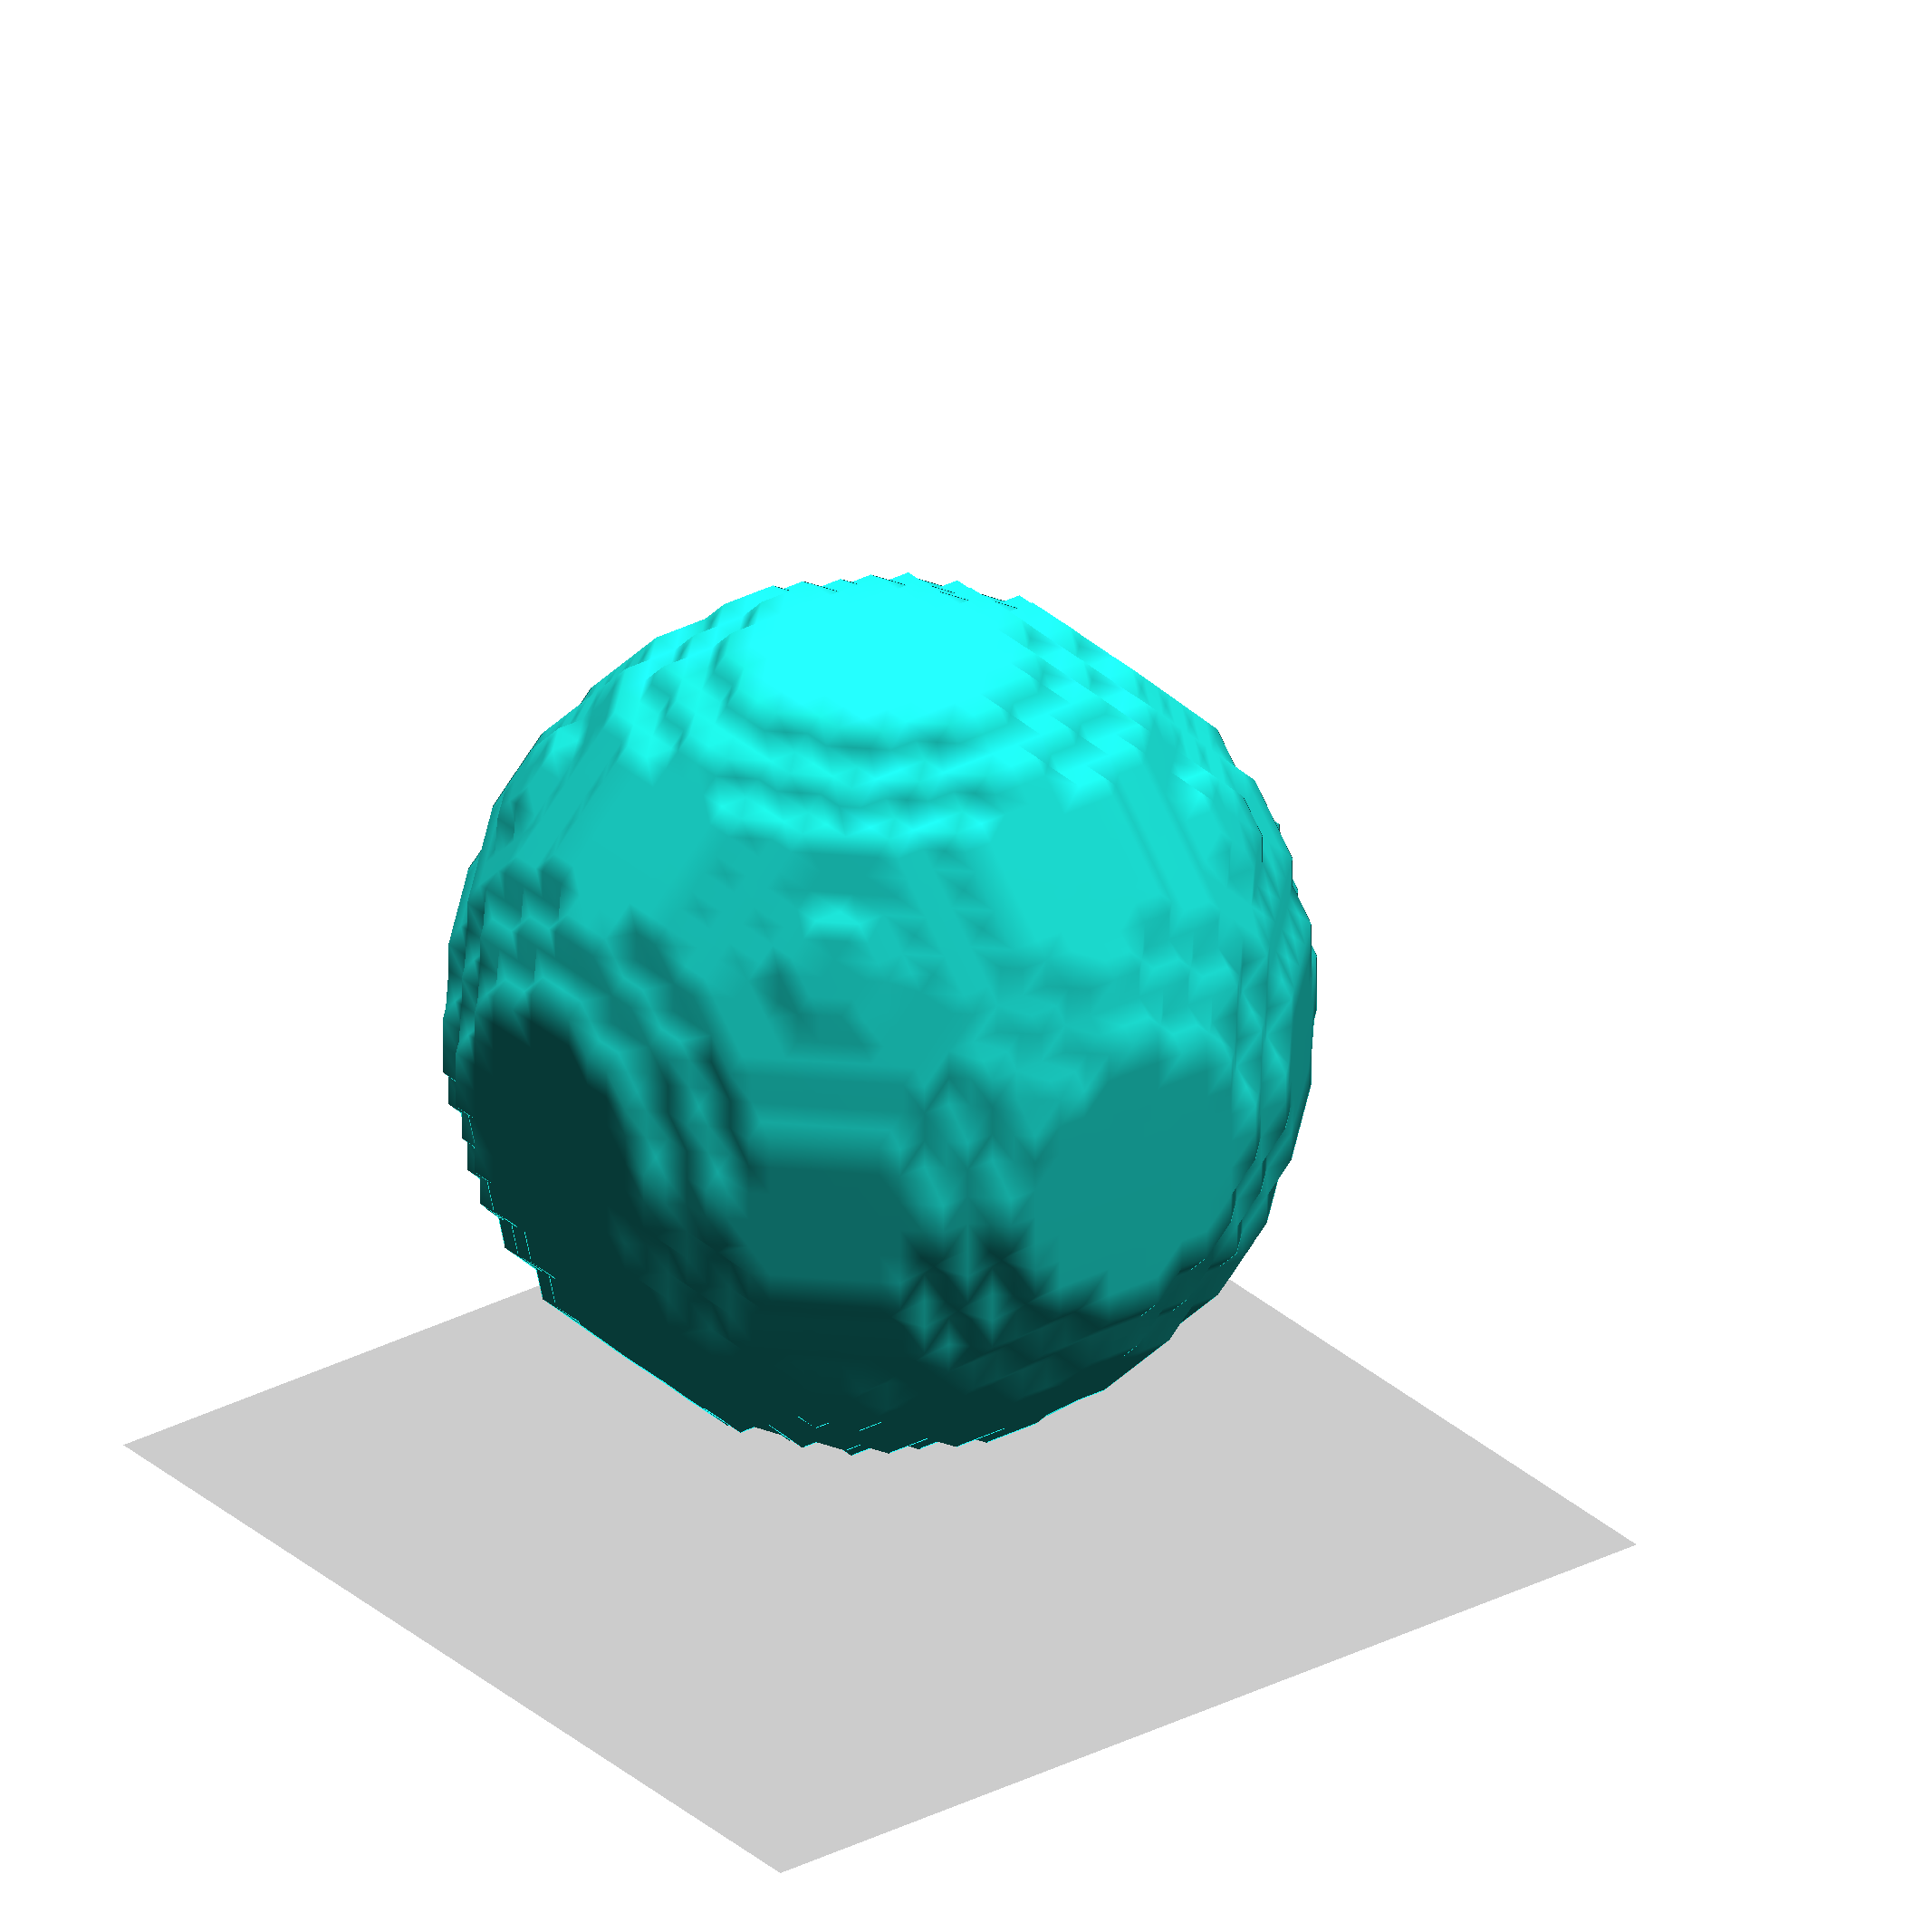
\includegraphics[width=0.18\linewidth]{chapter_background/img/binary_32x32x32.png} &
    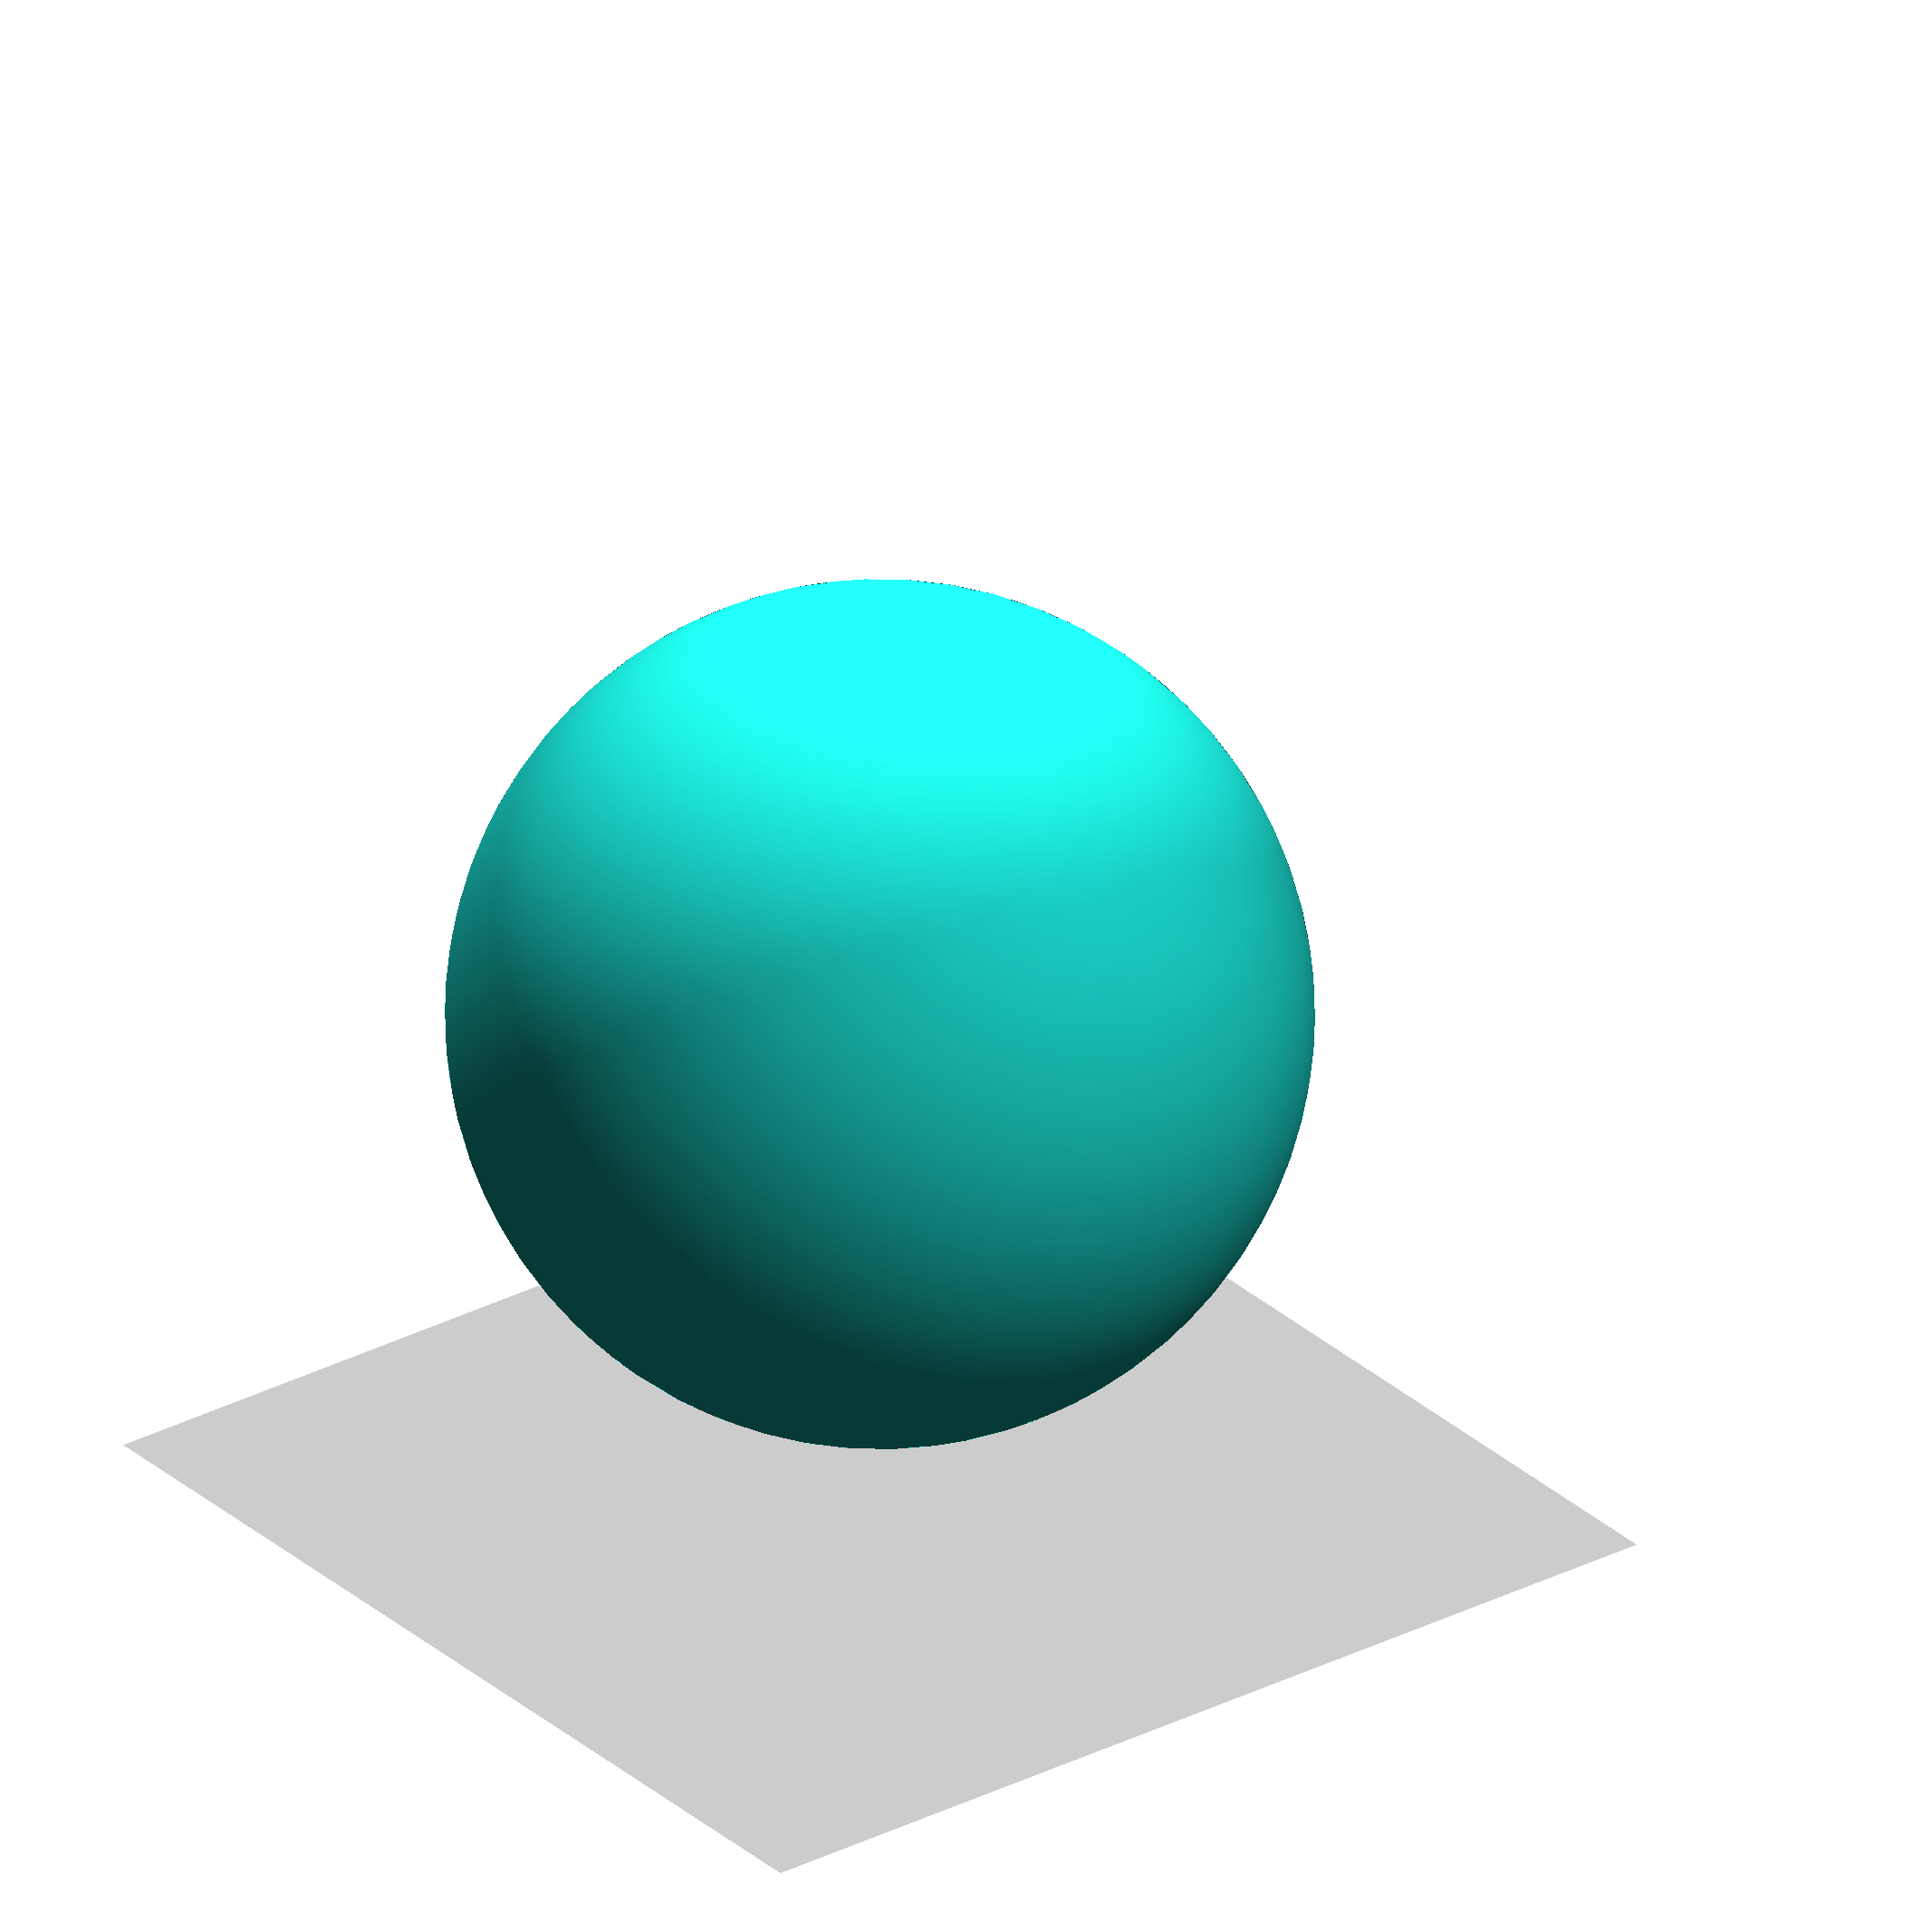
\includegraphics[width=0.18\linewidth]{chapter_background/img/real_32x32x32.png} &
    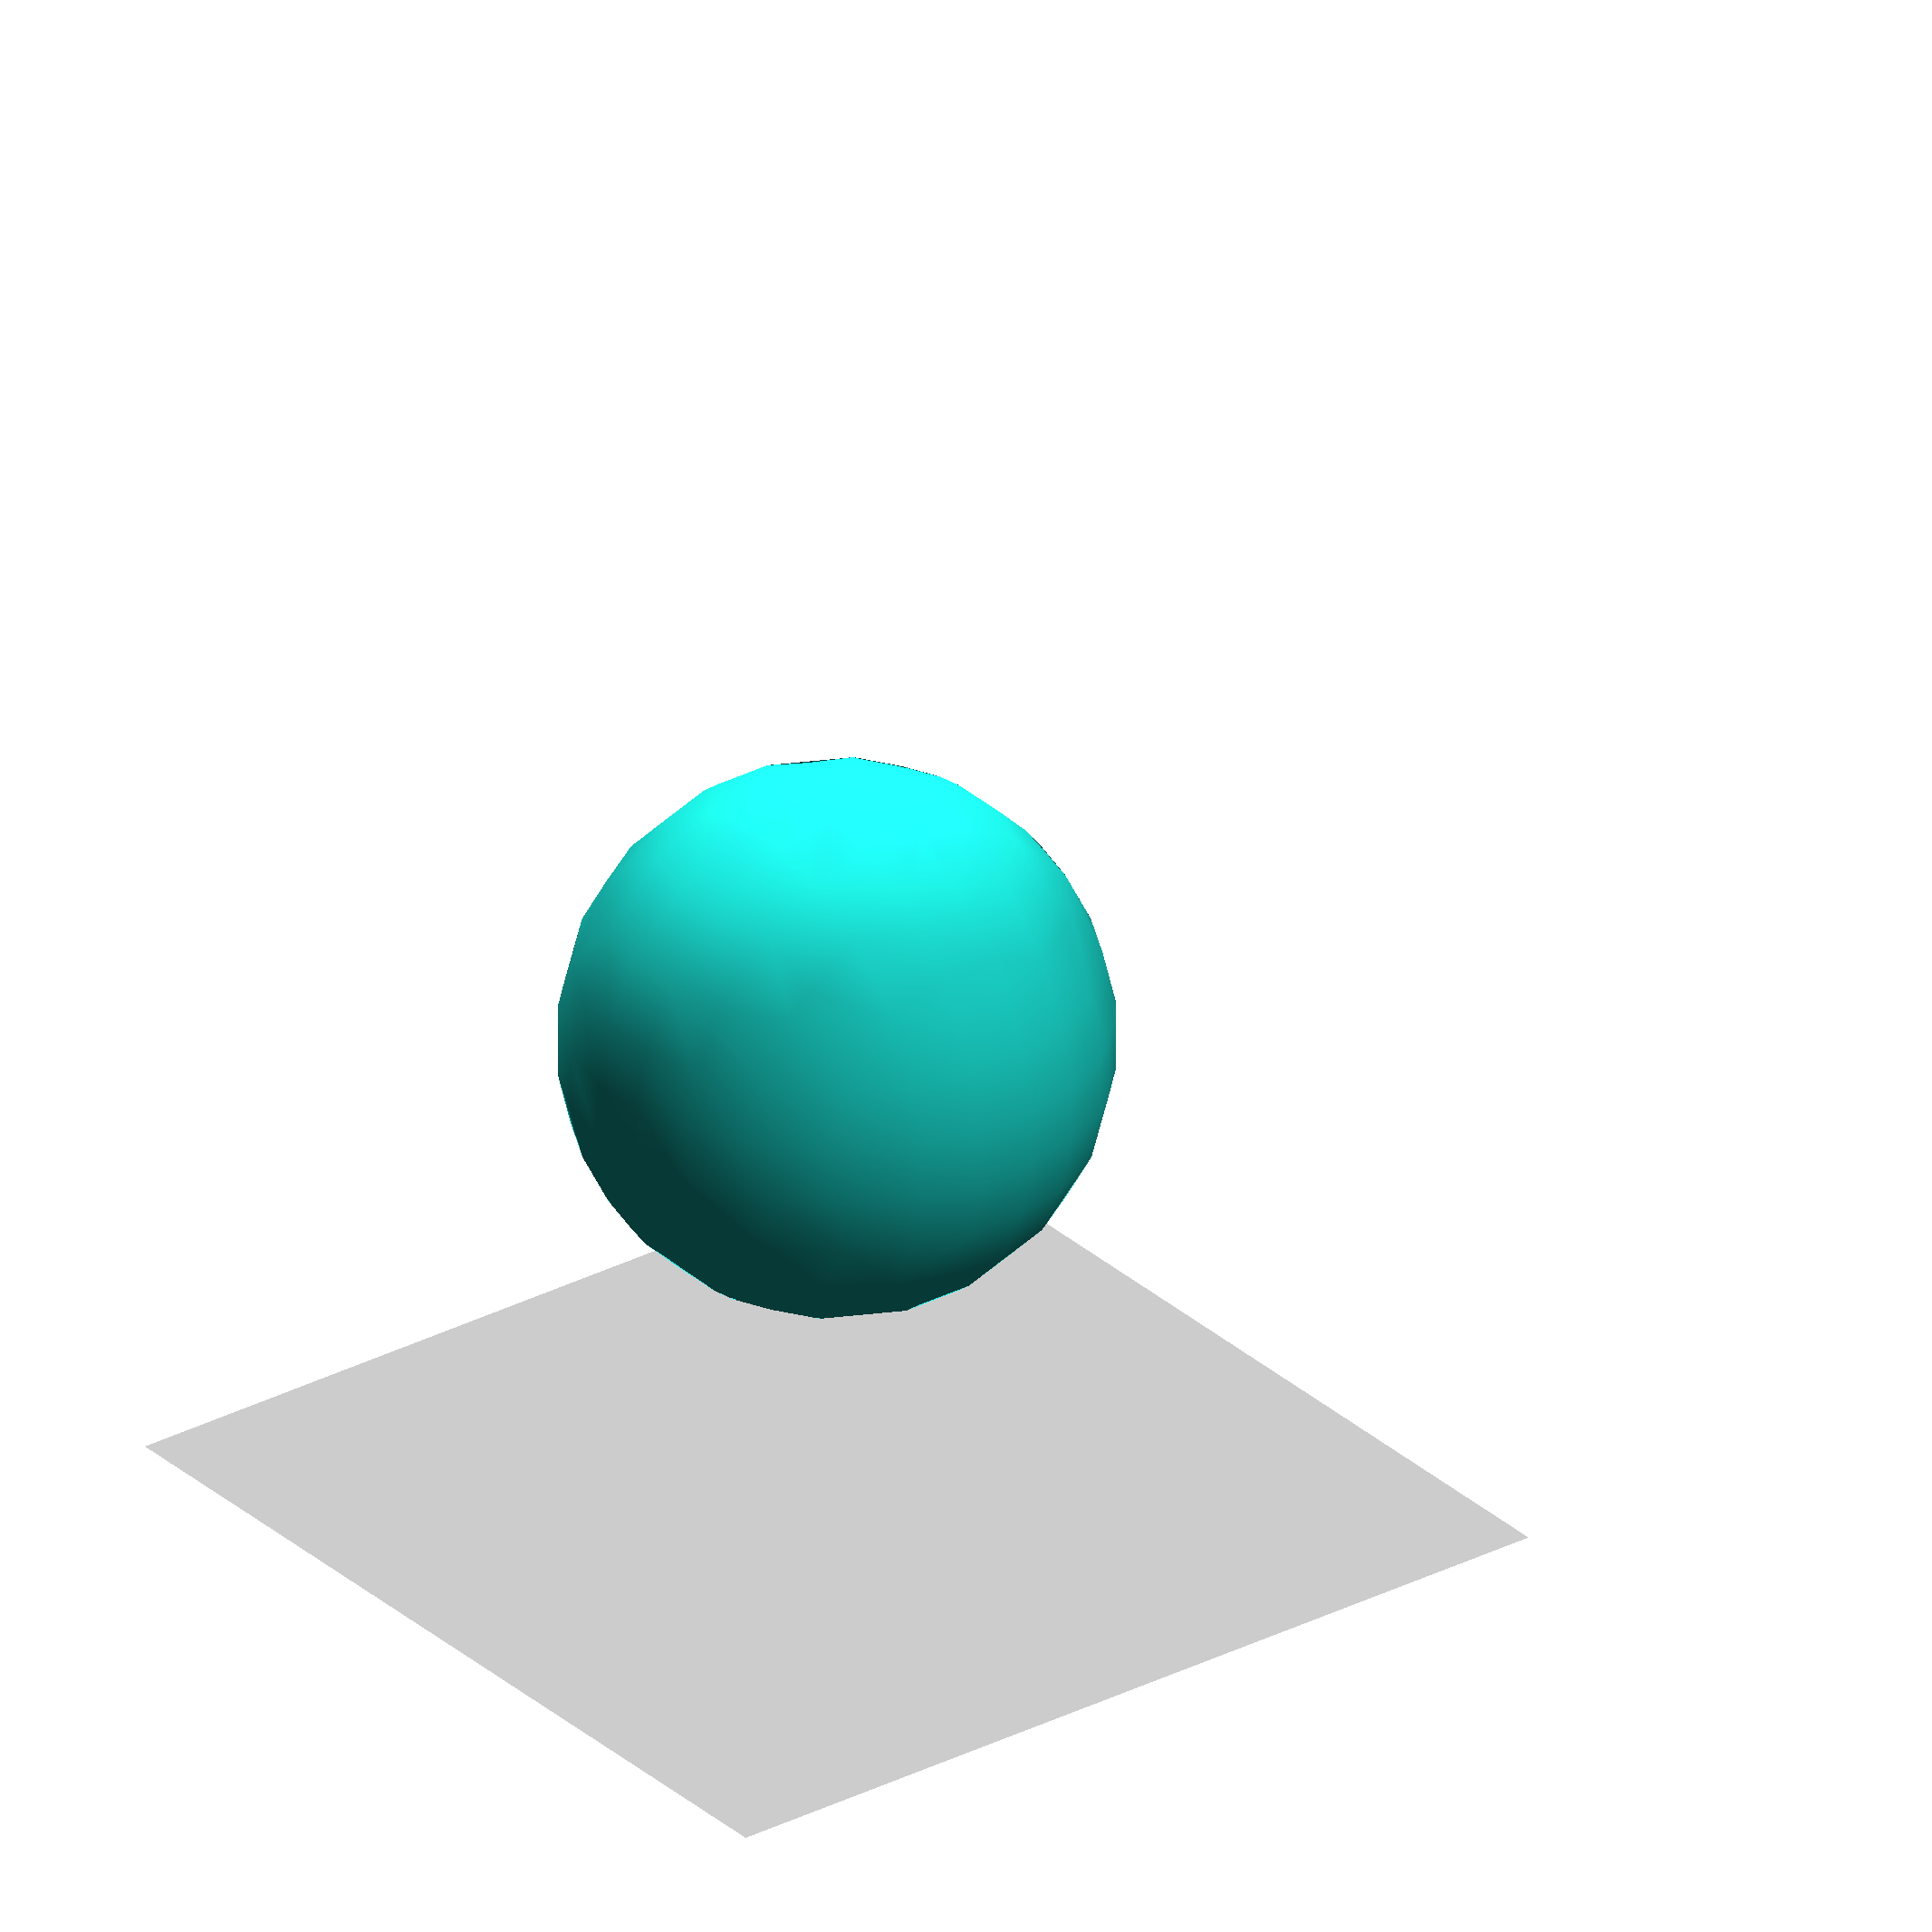
\includegraphics[width=0.18\linewidth]{chapter_background/img/real_16x16x16.png} &
    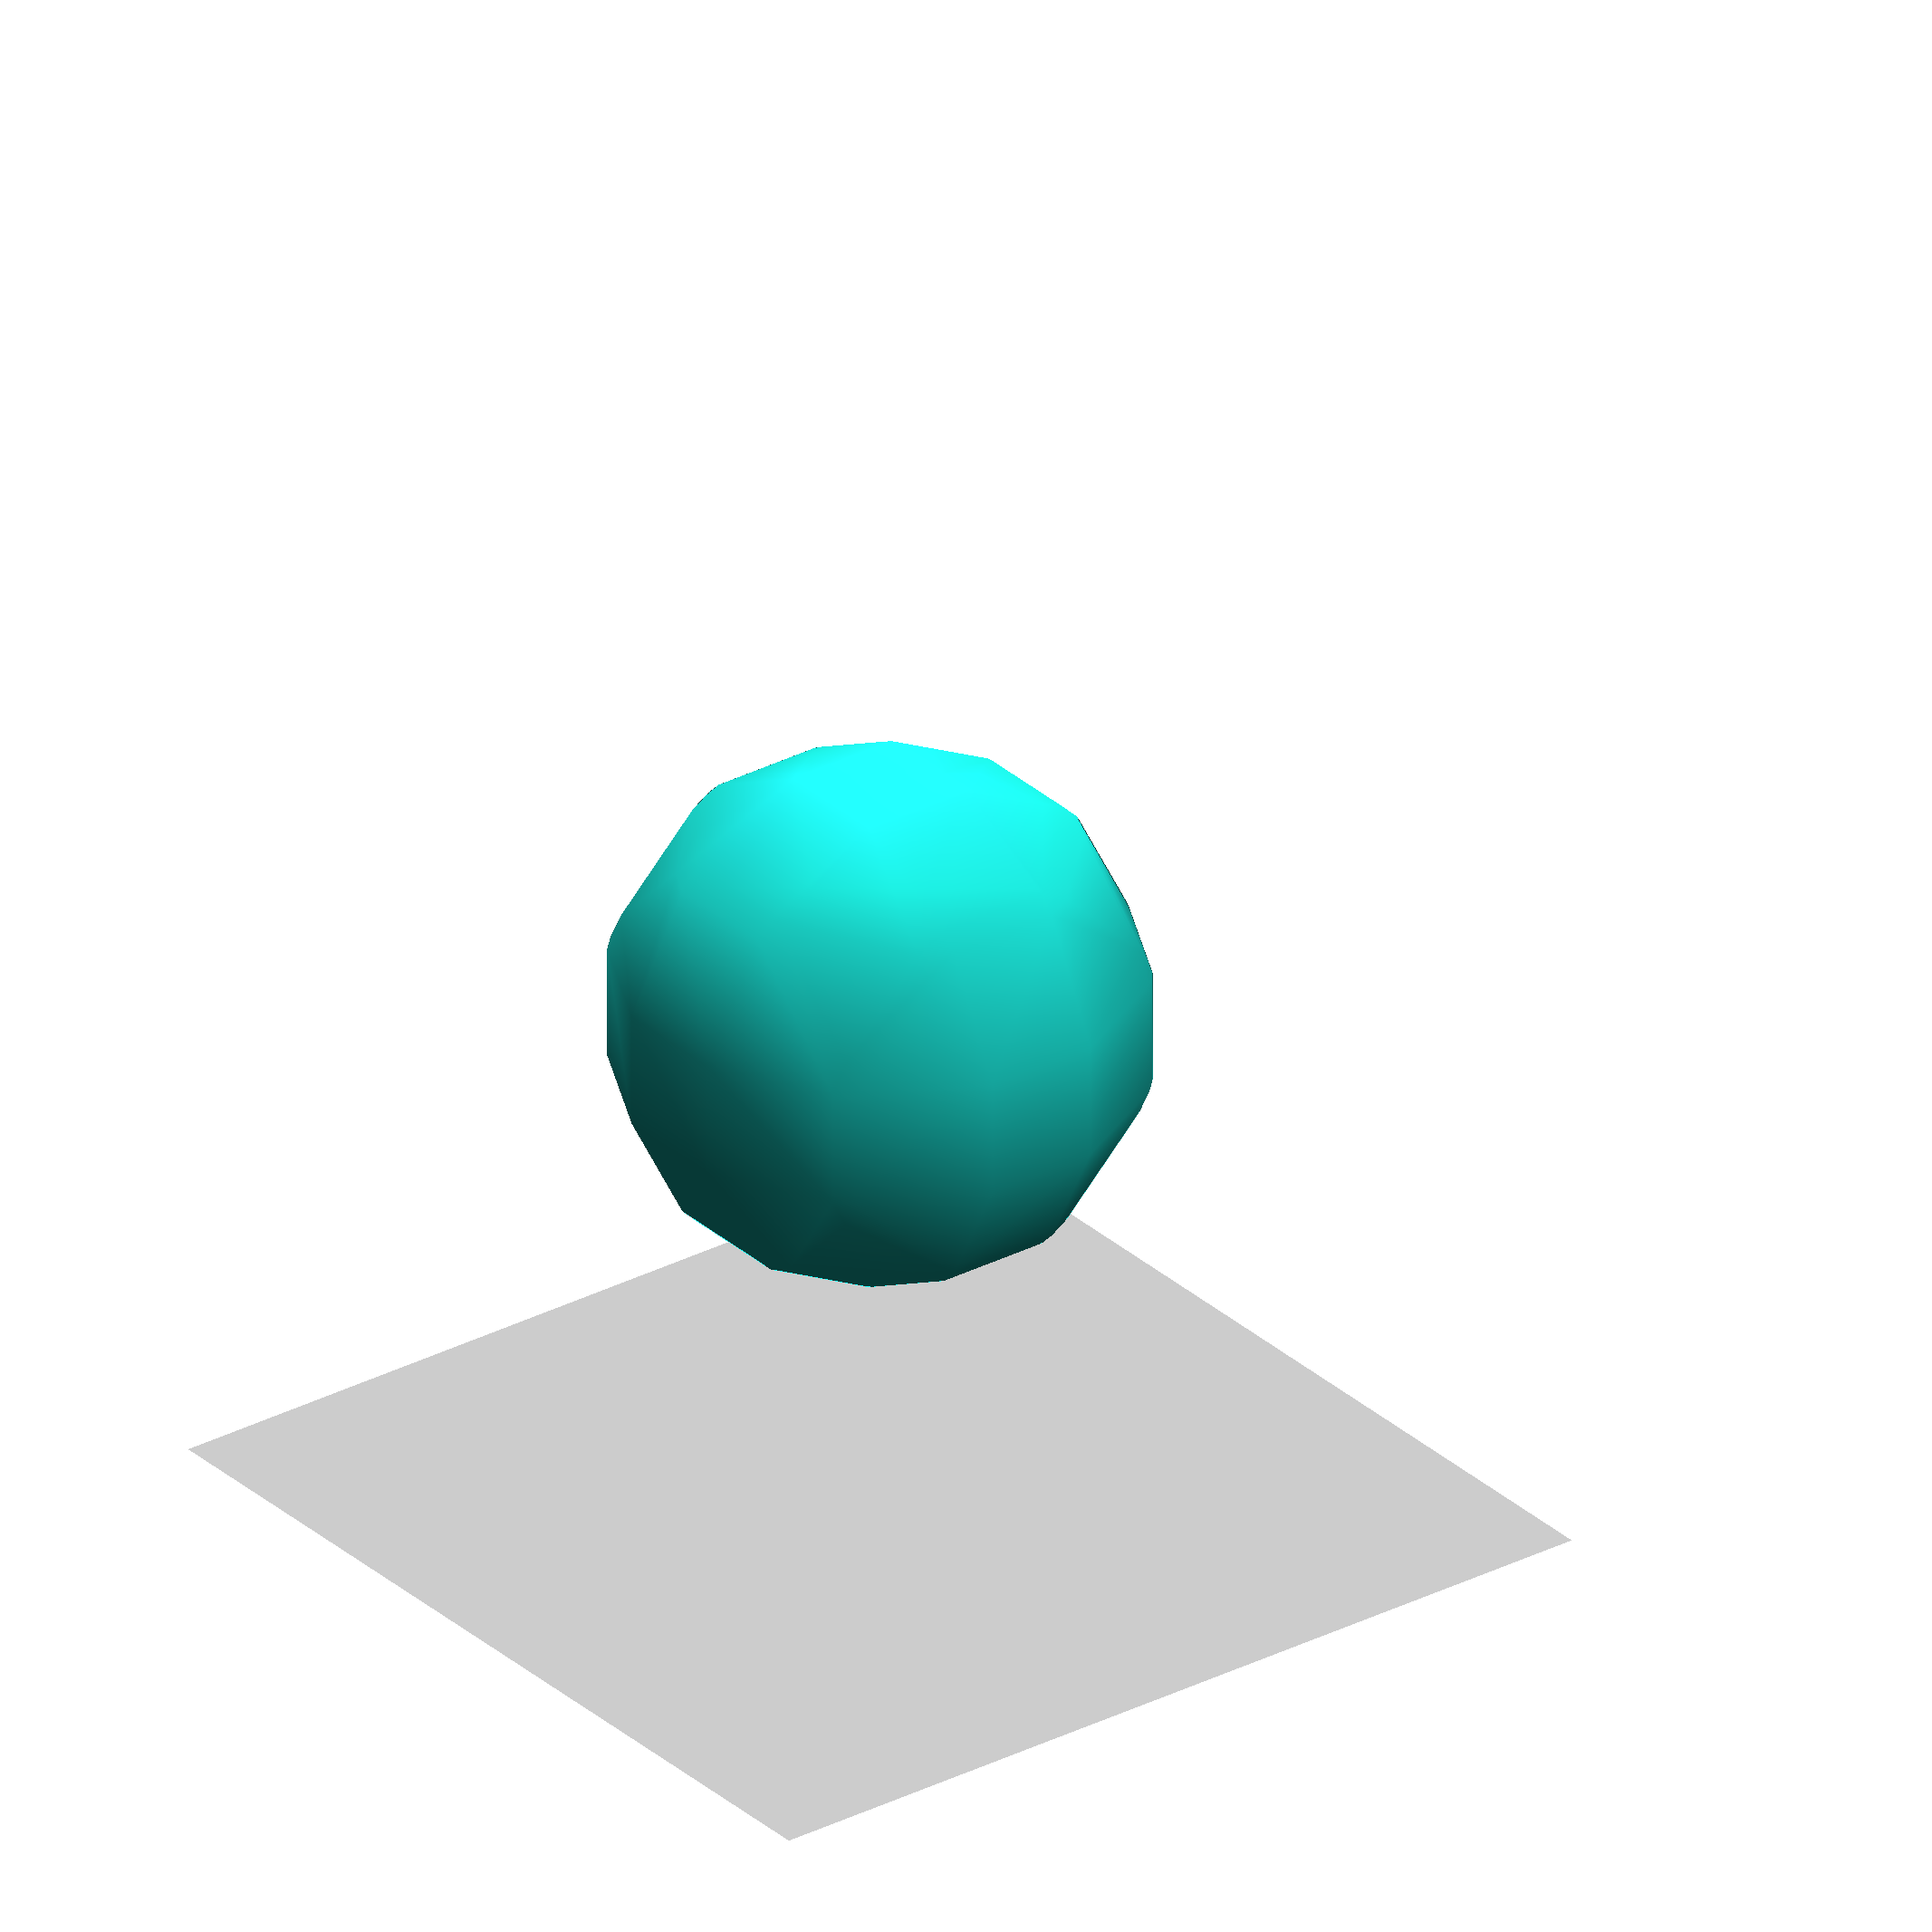
\includegraphics[width=0.18\linewidth]{chapter_background/img/real_8x8x8.png} &
    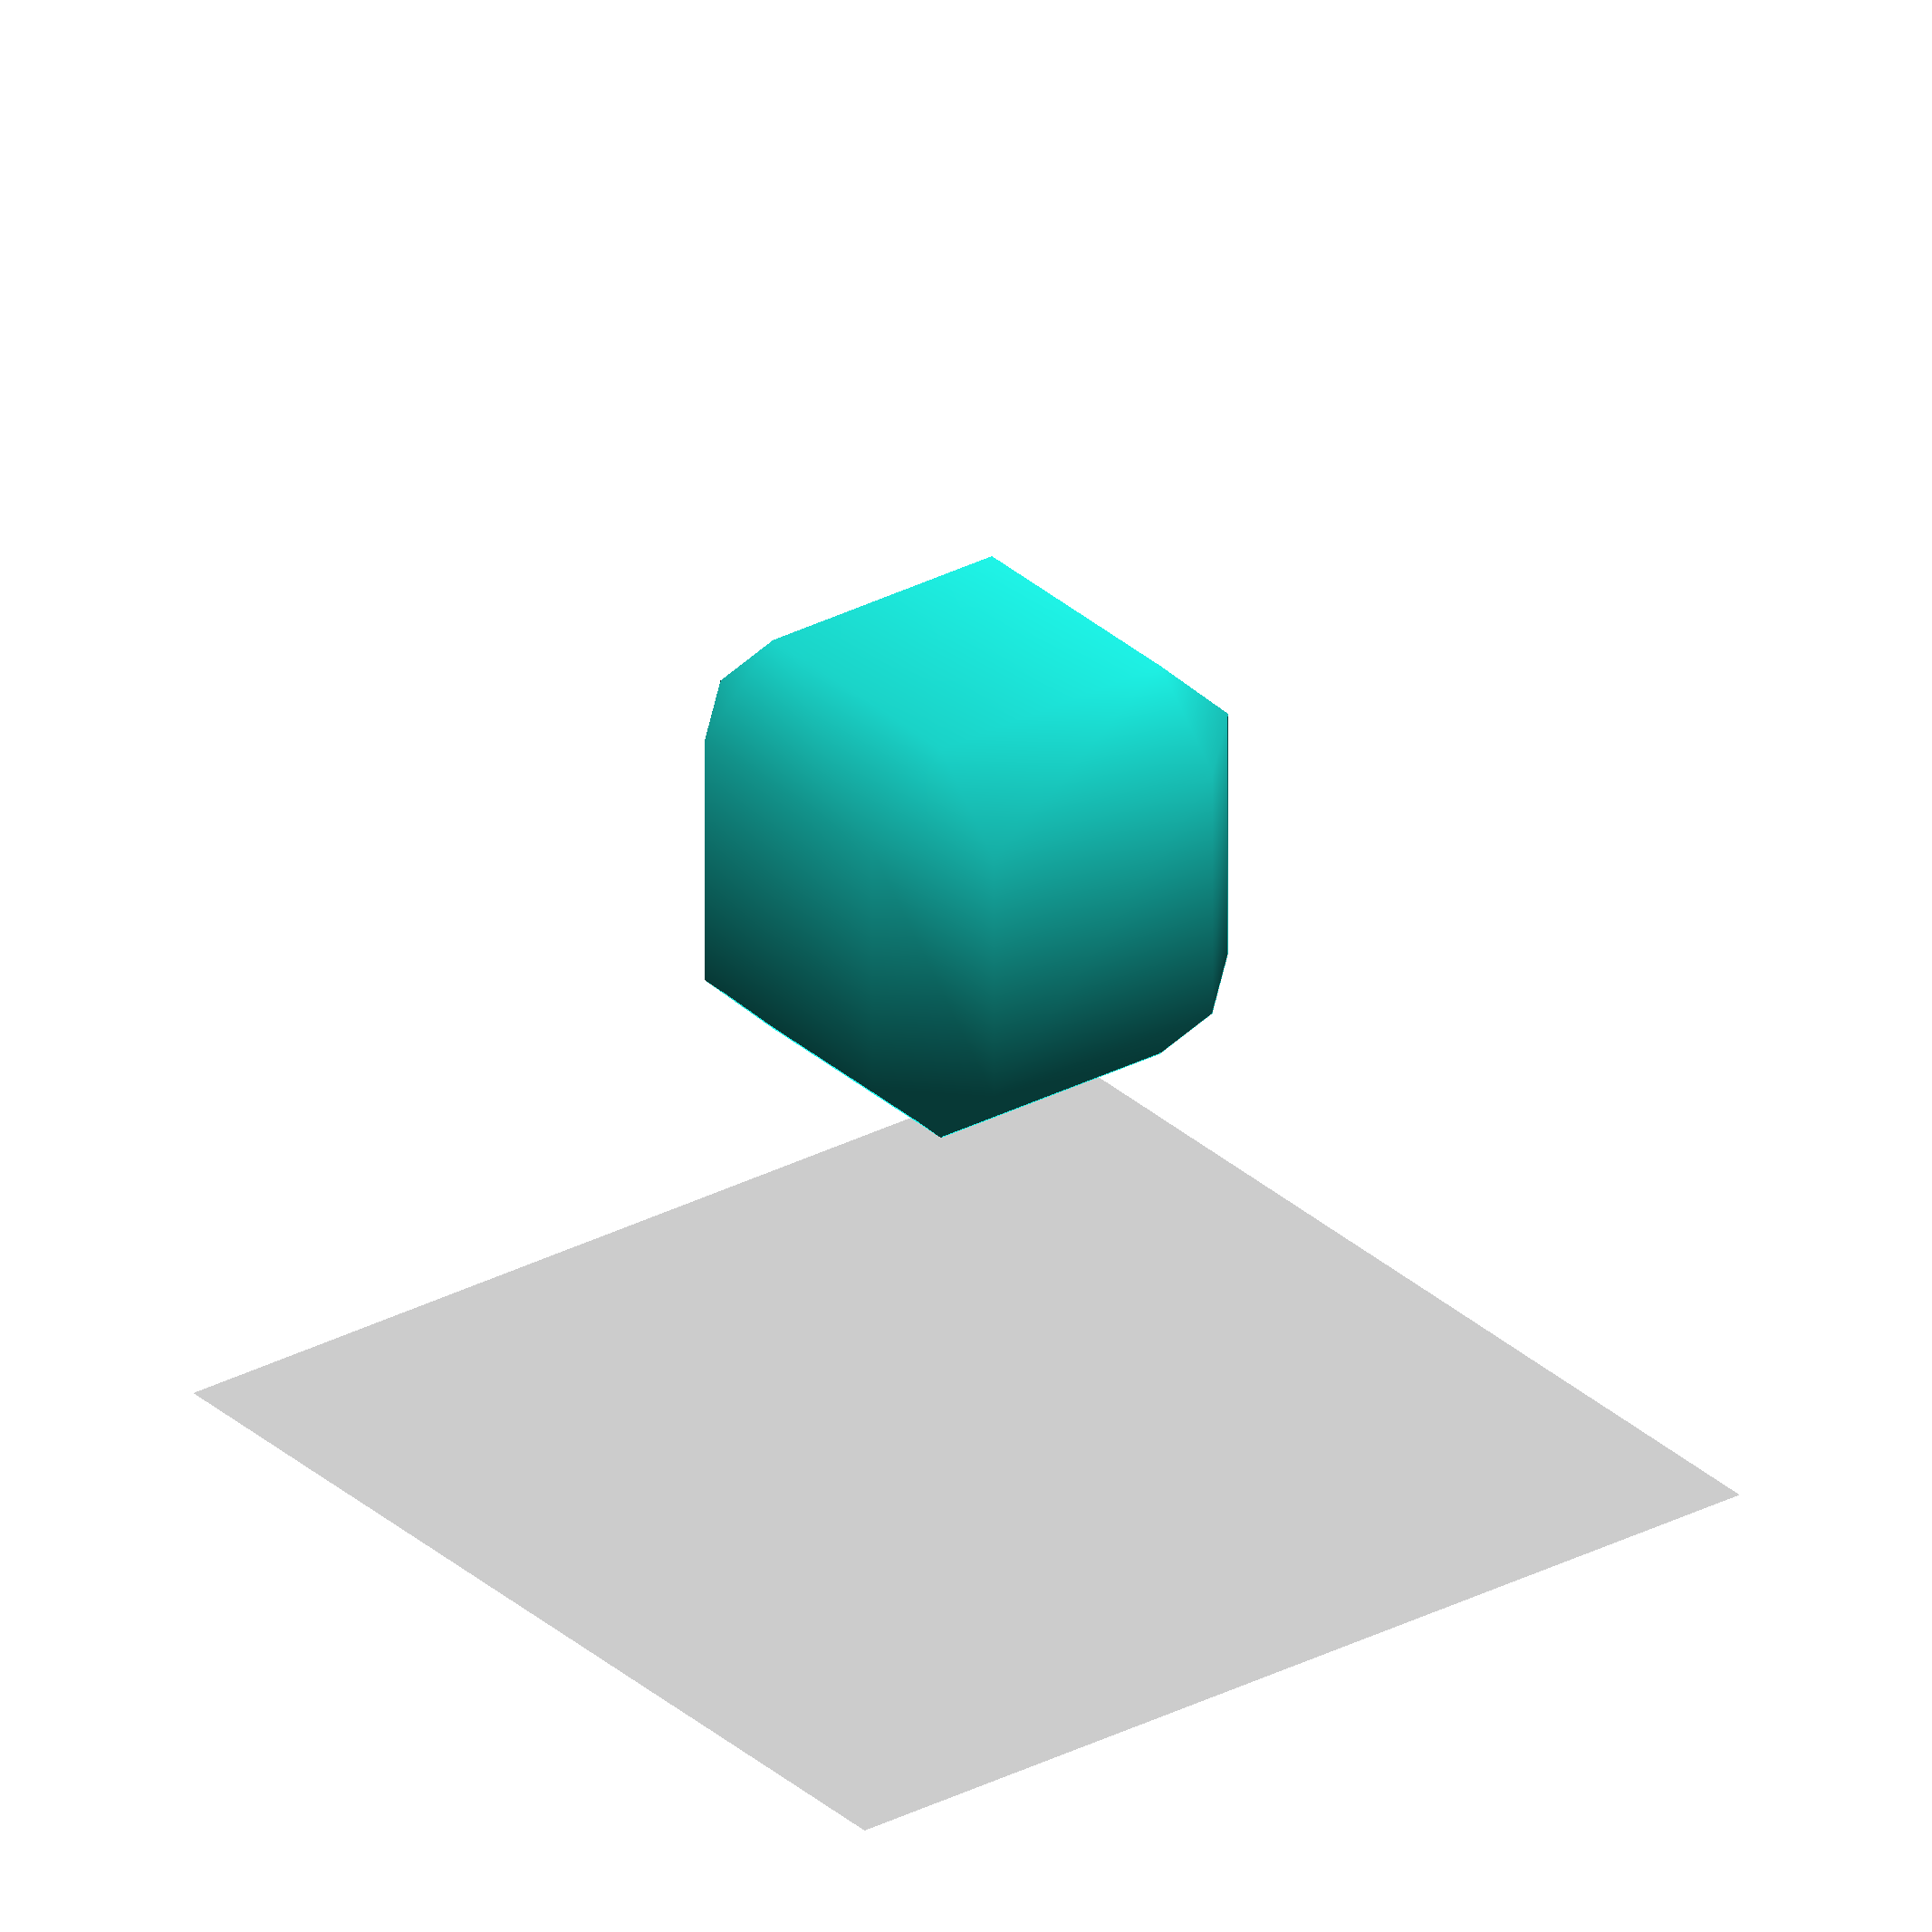
\includegraphics[width=0.18\linewidth]{chapter_background/img/real_4x4x4.png}
    \\
    Binary & Real & Real & Real & Real \\
    $32^3$ & $32^3$ & $16^3$ & $8^3$ & $4^3$ \\
  \end{tabular}
  \caption[Volumetric antialiasing at different resolutions]{A
    volumetric sphere, with and without antialiasing, at several
    different resolutions.}
  \label{fig:background:volquality}
\end{figure}

\subsection{Voxelisation}

The process of transforming a mesh into a volumetric structure is
referred to as voxelisation. Intuitively, this voxelisation process
discretises the mesh. It is no longer possible to reproduce a
non-integer form of the original mesh - a surface noticeably
constructed out of small cubes. Ideally, there should be minimal
visual degradation between viewing the original mesh and the voxelised
object, otherwise, how would it be possible to encode detail?  Just as
anti-aliasing is possible in 2D graphics, it is also possible with 3D
volumes. This is achieved by using real numbers inside a voxel,
instead of just a binary value.  This results in very low distortion,
provided the resolution is sensibly selected. This is shown in
Figure~\ref{fig:background:volquality}, where a sphere encoded using
binary values is clearly built out of cubes, where as even a small
real value volume remains representative.

Generating a 2D image from 2D vector graphics (such as polygons) is
called rasterisation. This involves tracing a ray while counting the
number of line intersections. If the count is odd, colour in pixel and
move onto the next. If the count is even, just move onto the next
pixel. Voxelisation follows a similar idea, except it is performed in
three dimensions instead of two. This is done by tracing rays through
the X, Y and Z planes separately to produce three separate
volumes. These volumes are then combined in some way, typically by
ensuring each XYZ coordinate has been set in at least two volumes
(voting). We show this visually in
Figure~\ref{fig:background:voltracing}, where error (shown in red) has
been introduced by only voxelising the Stanford
Bunny\footnote{http://graphics.stanford.edu/data/3Dscanrep} from a
single direction.

\begin{figure}
  \centering
  \begin{tabular}{ccccc}
    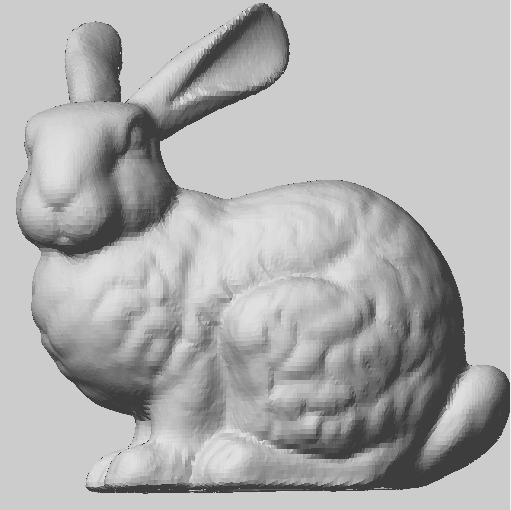
\includegraphics[width=0.17\linewidth]{imggen/vox_xyz/bunny_original.png} &
    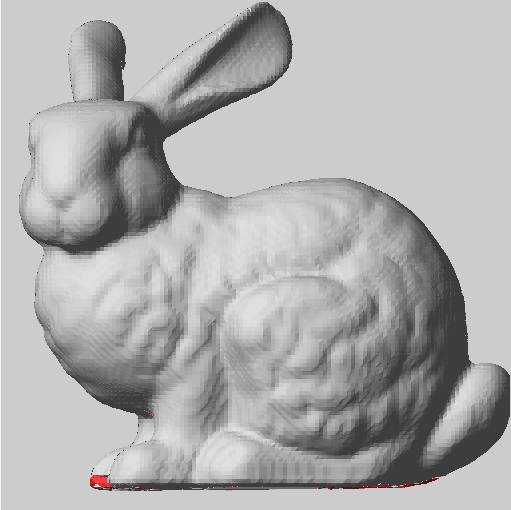
\includegraphics[width=0.17\linewidth]{imggen/vox_xyz/bunny_voxX.png} &
    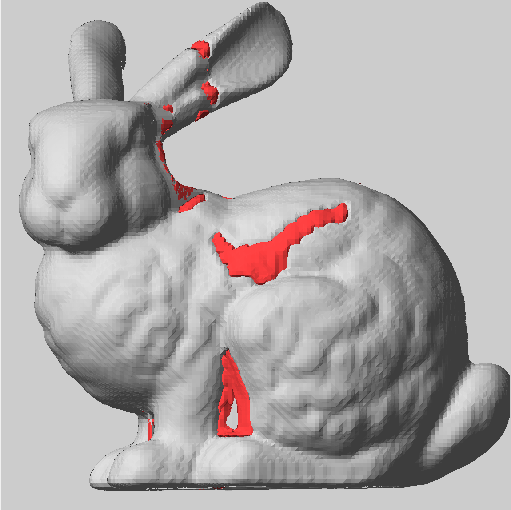
\includegraphics[width=0.17\linewidth]{imggen/vox_xyz/bunny_voxY.png} &
    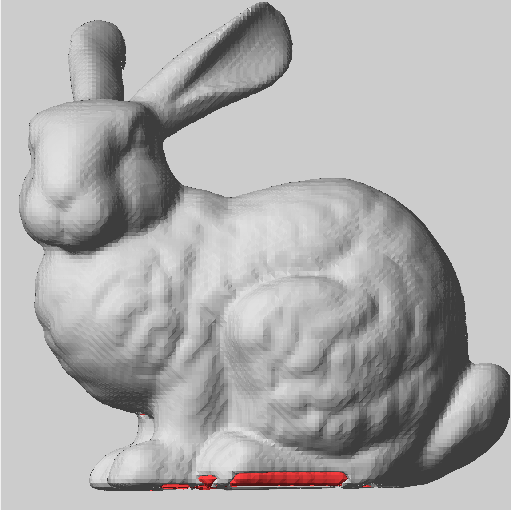
\includegraphics[width=0.17\linewidth]{imggen/vox_xyz/bunny_voxZ.png} &
    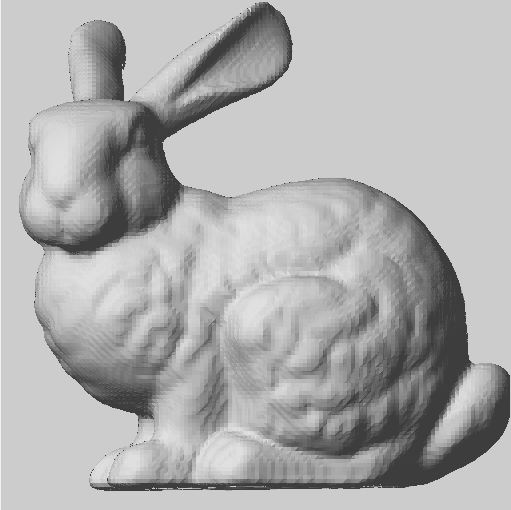
\includegraphics[width=0.17\linewidth]{imggen/vox_xyz/bunny_voxXYZ.png} \\
    Original & Voxelised & Voxelised & Voxelised & Voxelised \\
    Mesh     & Traced X  & Traced Y  & Traced Z  & Traced XYZ \\
  \end{tabular}
  \caption[Voxelisation error due to limiting ray tracing
  directions]{Voxelised results of the Stanford Bunny (original shown
    on left). The first three volumes have been voxelised by tracing
    from either X, Y or Z directions. The final volume (right most) is
    generated by voting. Red patches fill in voxels which have been
    missed. Each volume is $128^3$ in size.}
  \label{fig:background:voltracing}
\end{figure}

\subsection{Surface Extraction}

Surface extraction is the process of extracting a mesh which encloses
a 3D object represented in volumetric space. Occasionally such methods
require thresholds to extract separate regions of the volume, for
example, in an MRI scan, where the brain  needs to be visualised
independently of the skull (and hence, independently extracted from
the volume).

Perhaps the most popular method for computing the isosurface of a
volume is Marching Cubes~\cite{lorensen1987marching}, developed in
1987. The algorithm traverses through all voxels, using the value of
eight neighbouring voxels to form eight binary values, a single
byte. This byte can be used to lookup a known polygon configuration
from a table of $2^8 = 256$ entries. However, in the first version of
Marching Cubes, only 15 unique polygon configurations were
stored. This lead to cases of ambiguity when performing a lookup for
certain voxel configurations. The side effect of this is that meshes
would sometimes end up having holes in
them. In~\cite{chernyaev1995marching}, additional unique
configurations were proposed, leading to a total of 33. This removes
the ambiguity, and results in the meshes being closed or \textit{water
  tight}.


\subsection{Size, Compression and Formats}
\label{sec:background:volstorage}

There are many more factors which have to be considered when working
with volumetric representations of objects, as opposed to a standard
mesh.

To start with, the \textbf{size} of the volume (in terms of bytes)
grows much more rapidly than it would in a 2D image. In order to
represent a sensible amount of depth in a $128 \times 128$ image, a
volume of $128^3$ voxels is likely needed. If this is uncompressed and
encoded as bytes, it will require 2MB of storage. Scale this up to a
dataset of maybe 50,000 samples, use a slightly larger volume, and it
is clear that this may begin to cause problems.

One solution might be to compress the volumes. However, compression
introduces a significant computational overhead. It is a common trade
off between processing power, available storage and I/O speeds. While
compression of images has come a long way (even JPEG decoding is
hardware accelerated on some platforms now), the same is not true for
3D volumes. Generic file compression options are of course available
(Run Length Encoding, Huffman Coding and LZ77, just to name a few),
but on large volumes being read many times per second, the CPU could
easily become the bottleneck. In this work, we do not compress the
volumes and instead use large SSDs to store our volumetric training
data.

The format in which the volume is stored is another important
consideration. There are many formats for storing volumetric
data. Typically, these formats have been developed for the medical
field for use with MRI, CT scans and the like. As such, these formats
often include space for details such as patient information, along
with a metadata describing the resolution and bit depth of the
volumetric data. An argument can be made that none of this information
is required if the volumetric representation is used as an
intermediary state and doesn't have to be processed by
\textit{humans}. This applies to the work presented in this
thesis. The volumetric representation used in the work described
throughout this thesis is a contiguous array of bytes, which can be
very efficiently read into memory.

\section{Deep Learning Frameworks}

While designing and developing a framework to work with deep neural
networks \textit{might} be an interesting thought experiment for some,
it is far from the focus of this thesis. This section serves a brief
acknowledgement and justification for the choice of deep learning
framework used. The work presented throughout this thesis was
developed primarily under the Torch~\footnote{\url{http://torch.ch/},
  except for the work on facial part segmentation, which was developed
  under Cafe~\cite{jia2014caffe}}. There are a number of reasons for
this, but to name just a few:

\begin{enumerate}
\item Efficient GPU support. This is important, of course, in any
  framework intended for deep learning. Torch enables networks to be
  run in parallel (for speed) or sequentially (for additional memory)
  across multiple GPUs.
\item Elegant memory backend. Data can be loaded directly into memory
  and views can be applied to create $N$-dimensional Tensors without
  shuffling memory. This is very important when reading in large
  volumetric training samples.
\item Multithreading. The trade offs between I/O and CPU are discussed
  in more detail in Section~\ref{sec:background:volstorage}. However,
  regardless of how the data is optimised (in terms of compression or
  just raw data), volumes are big. Loading them sequentially and
  applying augmentation, even on very fast hardware, remains a
  computationally expensive task.
\end{enumerate}


%%% Local Variables:
%%% TeX-master: "../thesis"
%%% End:
 % Background
\chapter{Literature Review}
\label{chapter:literature}


This section attempts to provide a comprehensive literature review of
the works relevant to this thesis. This thesis focuses primarily on
the 3D reconstruction of human faces and bodies. Much of the
literature discussed in this chapter has an obvious
relevance. However, in the cases which are less obvious, connections
have attempted to be made with references to the relevant chapter and
section.

\section{Face Alignment}

Face alignment the process of detecting or aligning a set of facial
points to a facial image. Face alignment is a prerequisite to many 3D
face reconstruction methods - in fact, methods such
as~\cite{huber2016multiresolution} depend only on facial landmarks,
discarding the image entirely. Our own methods optionally makes use of
these landmarks to assist in the 3D reconstruction process. These are
discussed in detail in Chapters~\ref{chapter:face} and~\ref{chapter:seg}.

Until recently, the highest performing methods for face alignment were
based on a cascaded regression approach. These methods estimate the
location of facial landmarks by applying a sequence of
regressors. Provided to these regressors is typically
SIFT~\cite{lowe2004distinctive} and other hand selected
features. These regressors are applied in a cascaded fashion where the
input to regressor $k$ is the estimate from regressor $k-1$. More
details of such approaches to face alignment can be found
in~\cite{sanchez16,cao2014facewarehouse,xiongsupervised,zhu2015face,tzimiropoulos2015project}.

The remainder of this section will focus on deep learning based
approaches to face alignment. A CNN casecade is presented
in~\cite{sun2013deep} to directly produce the landmark
locations. Similarly in~\cite{bulat2016two}, the authors propose a
method for 3D face alignment by first detecting the 2D landmarks using
heatmap regression. If desired, the process can be stopped
here. Optionally, this stack of heatmaps is passed through a second
network, this time for regression, accompanied by the original input
image. The output of this second stage is 68 $(x, y, z)$
landmarks. A multitask approach is proposed in~\cite{zhang2014facial},
regressing the location of the facial landmarks while performing
facial attribute classification.

Many CNN based alignment methods estimate the facial landmarks by
regressing a 2D Gaussian on top of each landmark
location~\cite{bulat2016two,bulat2017far,mahpod2018facial,kowalski2017deep,merget2018robust}.
This spatial approach is commonly referred to as heatmap
regression. One such example is the extension to~\cite{bulat2016two}
in~\cite{bulat2017far}, where the second regressor is replaced with a
CNN producing a 3D heatmap representation. A similar heatmap based
approach was used in a multi-stage approach described
in~\cite{kowalski2017deep}, where the landmark detections are refined
after each stage. Between each stage, the \textit{current} landmark
prediction and some generated features are passed. At the beginning of
each stage, the inputs are transformed using the landmarks to make the
problem less challenging.

An indirect approach is discussed in~\cite{zhu2016face}, where a 3DMM
is first fitted, from which 3D landmarks are taken. This work is
discussed in further detail in
Section~\ref{chap:literature:sec:face_recon}. A similar idea is
propsed in~\cite{jourabloo2016large}, where a dense 3D model is fit to
the face first.

\section{Face Reconstruction}
\label{chap:literature:sec:face_recon}

3D face reconstruction is the process of estimating the 3D geometry of
a face. This is typically from one or more images, but methods relying
on video, depth data, and landmarks also exist. Arguably the most
popular approach to estimating the 3D geometry of the human face is
using 3D Morphable Models (3DMM). These models consist of a small
number of parameters which adjust facial properties such as shape,
pose and expression. Such methods
include~\cite{jourabloo2016large,huber2016multiresolution,zhu2016face,liu2016joint,tran2018extreme,jiang20183d,jiang2018pose}.

In particular,~\cite{jourabloo2016large} use a cascade of CNNs, which
first regress the camera projection, followed by the pose, followed by
shape and expression. Additionally,~\cite{jourabloo2016large} extract
features from their model fitting which can assist in facial landmark
localisation. A method capable of working with models of different
resolutions is proposed in~\cite{huber2016multiresolution}, along with
several models of different resolution, ranging from roughly 30,000 to
3500 vertices. This method does not use a CNN, instead regressing
parameters for shape and pose from the landmarks only, by minimising a
cost function which evaluates the fitting.

Constraining the pose, shape and (optionally) appearance into a small
number of parameters has the undesirable side effect of being unable
to capture finer details, such as wrinkles and
bumps. In~\cite{tran2018extreme}, a CNN is used for 3DMM fitting,
followed by a refinement step which iteratively improves the finer
details. However, during this iterative refinement, the correspondence
between vertices, as well as the scale and spatial location of the
fitting is lost. Another iterative approach attempting to
\textit{also} recover both the 3D geometry and facial landmarks is
described in~\cite{liu2016joint}. For initialisation, the method
passes the image and a mean set of facial landmarks. These landmarks
are gradually refined while learning a 3D to 2D mapping, which updates
the 3D face shape. Unlike the aforementioned methods, our own method
(described in Chapter~\ref{chapter:face})~\cite{liu2016joint} does not
estimate the facial pose, and as such always produces a frontal
reconstruction.

The data required for training 3D reconstruction methods typically
consists of an image with a corresponding 3D scan and can be difficult
to obtain. \cite{richardson20163d} avoid this issue by generating
synthetic training data, composed of renderings of randomly generated
3DMM with corresponding meshes. Faces are rendered under random
lighting conditions and projected only the image plane. An incremental
fitting method is then used during inferences. Synthetic data was also
used for training a general purpose 3D reconstruction
method~\cite{li2015joint}. Methods trained using synthetic training
data often fail on real or ``in-the-wild'' images due to unrealistic
renderings or constrained lighting.

A partially synthetic approach to 3D face reconstruction (indirectly
for face alignment) is proposed in~\cite{zhu2016face}. The method used
a single CNN that is iteratively applied to estimate the model
parameters using as input the 2D image and 3D shape and pose
representation from the previous iteration. The network consists of
four convolution layers and two fully connected layers. The first two
convolutions share parameters for memory efficient feature
extraction. This shape and pose representation can best be summarised
as a depth map of the fitting generated by parameters from the
previous iteration. The training data is augmented by artificially
rotating faces between $\{-90, 90\}$ degrees using groundtruth
parameters for a frontal fitting.

A method which performs 3D reconstruction from video is presented
in~\cite{suwajanakorn2014total}, which can also work from a set of
static images. The method combines their proposed 3D flow estimation
algorithm with a Shape from Shading (SfS) method. The method first
estimates the facial pose, which is used to rotate an average face
shape to the correct pose. For each frame, 3D flow updates the mesh,
which both refines the detail, and updates aspects such as expression
and pose. Another Shape from Shading approach is proposed
in~\cite{jiang20183d}, which first aligns a coarse face reconstruction
using 2D landmark detections. This coarse model is then
\textit{corrected} using medium scale features from the
image. Finally, the shape from shading step refines the mesh and
introduces finer details.

Our method for 3D face reconstruction, described in
Chapter~\ref{chapter:face} is very different to the aforementioned
methods. First, our method does not rely on a 3D shape model for
either the pre-processing or ``fitting'' procedure, instead we rely on
a volumetric representation. This avoids the requirement to find
correspondence between vertices, which is a challenging problem in
itself. Second, our method is direct, producing a volumetric
representation of the facial geometry in just a single step. Third,
unlike~\cite{tran2018extreme} we do not lose any pose or scale
information, and show potential for detailed reconstruction,
demonstrated in Chapter~\ref{chapter:human} on human bodies.



\section{Human Pose Estimation}

While this thesis does not focus on pose estimation, in
Chapter~\ref{chapter:human}, we present our method for 3D human body
reconstruction as an extension to our 3D face reconstruction
work. Human pose estimation is optionally used as guidance for this
method in a similar fashion to face alignment being used as guidance
to 3D face reconstruction.

Modern approaches to estimating human pose are based on methods
employing CNNs. These methods generally fall into one of two
categories. The first is to directly regress the coordinates of the
joints using an L2 (or similar) loss, see for
example~\cite{li20143d,park20163d,tekin2016structured,tekin2016direct,zhou2016deep,chen2016synthesizing,ghezelghieh2016learning,toshev2014deeppose,tompson2014joint}. In
particular,~\cite{park20163d} estimates the 3D pose by combining the
2D predictions with image features. An autoencoder is employed
in~\cite{tekin2016structured} to constrain pose to something
plausible. Similarly,~\cite{zhou2016deep} have the same goal but
achieve this by using a kinematic model. Synthetic training data is
used for the full training procedure in~\cite{chen2016synthesizing},
to ensure that the network is trained with accurate data. However,
in~\cite{ghezelghieh2016learning}, they only augment their existing
training set with synthetic data. ~\cite{toshev2014deeppose} propose
an iterative method, in which images are first passed through an
initalisation CNN. The output from this is then combined again with
the input image and passed through a second CNN multiple times
iteratively.  In~\cite{tompson2014joint}, a multi-resolution CNN is
trained jointly with a Markov Random Field, helping to refine the
prediction from the CNN by constraining pose. An iterative method is
presented in~\cite{carreira2016human}. However,
unlike~\cite{toshev2014deeppose}, which directly outputs the locations
of the joints after each iteration,~\cite{carreira2016human} outputs a
displacement vector for each joint. The displacement is applied and
the points are \textit{rendered} to heatmaps, which fed into the
network again for the next iteration. For the first iteration, a mean
pose is provided to the network.

The second approach to CNN based human pose estimation is to regress
heatmaps, as done
in~\cite{newell2016stacked,pfister2015flowing,zhou2016sparseness,pavlakos2017coarse,mehta2017vnect,zhao2018through}. In
these methods, an intensity value is regressed for each pixel, giving
a likely hood of the joint in that pixel.
In~\cite{newell2016stacked}, a novel ``stacked hourglass'' network is
proposed. This architecture gradually reduces and increases the
spatial resolution while combining features from different
scales. Combining these features from different scales allows the
network to produce better predictions as both global and local context
is available to the last few layers of the network. A loss function is
used between each hourglass, which allows the network to refine and
reevaluate the pose as it passes through the network (similar to idea
of iterative methods,
e.g.~\cite{toshev2014deeppose,carreira2016human}). This architecture
in particular, despite intended for human pose estimation, has
strongly influenced our work on 3D reconstruction, discussed further
in Chapters~\ref{chapter:face} and~\ref{chapter:human}. A 3D heatmap
is regressed in~\cite{pavlakos2017coarse}, which is a similar idea to
our own 3D reconstruction, but for pose, not geometry. A part based
heatmap regression method is presented in~\cite{mehta2017vnect}.

In~\cite{pfister2015flowing}, video is used
instead of a single image. The method accepts an arbitrary number of
neighbouring frames for each time $t$. Features between frames are
combined using what they call ``Spatial Fusion Layers''. For each
frame at time $t$, a pose heatmap. Optical flow is used from the
neighbouring frames to time $t$ to refine the prediction at. Finally,
in~\cite{zhao2018through}, the authors present their method for
\textit{seeing through walls}, by using a standard CNN trained on 2D
radio frequency heatmaps, for both horizontal and vertical
polarizations.



\section{Human Body Reconstruction}


Many human reconstruction methods estimate the geometry from one or
more images. For
example,~\cite{balan2007detailed,grest2005human,guan2009estimating}
fit a model based on a single RGB or grey scale images. In particular,
\cite{grest2005human} fit a skeleton model to the image by estimating
the scale and pose of each body part
separately. In~\cite{guan2009estimating}, they fit a shape model
initialised by a user clicking on separate body parts, assisted by a
segmentation mask. Another shape model based approach is proposed
in~\cite{balan2007detailed}, using the SCRAPE
model~\cite{anguelov2005scape}, which is fitted with a stochastic
optimisation step. A general shape fitting method for reconstruction
is proposed in~\cite{chen2010inferring}, where two Gaussian models are
used - one for shape and one for pose, by solving non-linear
optimisation problems. The authors demonstrate this method on human
bodies and sharks. In~\cite{jiang20103d}, a single image and
corresponding landmarks are used to lookup a similar human pose using
a kd-tree, containing about 4 million examples. A method intended for
multi-instance model fitting from a single image is described
in~\cite{Zanfir_2018_CVPR}.

Several methods aim to estimate the 3D geometry using only the
landmarks extracted via human pose
estimation~\cite{bogo2016smplify,ramakrishna2012reconstructing}. Particularly,
SMPLify~\cite{bogo2016smplify} (which uses the SMPL
model~\cite{loper2015smpl}), was extended to also include further
guidance from an segmentation mask
in~\cite{varol2017learning}. However, such an approach will never be
able to capable of regressing finer details, unless information from
the image is also captured.

Aside from SCRAPE~\cite{anguelov2005scape} and
SMPL~\cite{loper2015smpl}, mentioned earlier, Dyna, the shape model
capable of capturing large variations in body shape is presented
in~\cite{Dyna:SIGGRAPH:2015}, but without an accompanying fitting
method from a single image. A very recent shape model called Total
Capture~\cite{Joo_2018_CVPR} captures many aspects of the body which
are typically ignored by other shape models, including the face and
hands.

The work we present in Chapter~\ref{chapter:human} is different from
all of the aforementioned methods in that we do not regress parameters
for a shape model, nor do we regress the vertices directly. Further
more, our method skips the model generation step entirely, which
avoids the need to find dense correspondence between all training
examples. Instead, we constrain the problem to the spatial domain, and
directly regress the 3D structure using spatial convolutions using a
CNN, via a volumetric representation from which the full 3D geometry
can be recovered.


\section{Semantic Segmentation}

Semantic segmentation is the process by which pixels of an image are
labelled by the objects contained in the image. For example, all dogs
may be labelled as red, while cats may be labelled as green. In order
for this to work, context is required, both locally and
globally. Global context tells us what is in the image and roughly
where a particular object may be located. Local context then refines
this global information, defining boundaries between classes with
greater precision.

Classical approaches to semantic segmentation involved first
segmenting the image using statistical models, followed by
individually classifying the segmented objects. See for
example~\cite{arbelaez2012semantic,carreira2012semantic}, which use a
Conditional Random Field (CRF) to separate the image. However, these
methods generally struggle to adequately incorporate high and low
level feature descriptors necessary for accurate segmentation and
labelling.

CNNs drastically changed the landscape of semantic segmentation. The
first work producing satisfactory semantic segmentation was the Fully
Convolutional Network (FCN) described in~\cite{long2015fully}, which
is based on VGG-16~\cite{simonyan2014vgg}. In this work, information
is forked from different layers throughout the network. Each fork is
used to produce an intensity map for all known class (initially 59,
targeted at the PASCAL VOC 2010
dataset~\cite{everingham2010pascal}). Forks earlier on in the network
provide very detailed but noisy predictions about the location of
classes, where as the latter forks are have very little noise, but can
only approximate the location of a class. A diagram of the structure
of FCN is shown in Figure~\ref{fig:background:fcn}. FCN was not
intended to be trained from scratch. Instead, training was initialised
from the parameters of VGG-16, once the network had been trained on
the ImageNet dataset~\cite{krizhevsky2012imagenet} for the task of
classification. The parameters in the last few layers of the network
were reshaped from linear layers into a $1\times 1$ convolution. An
interesting side effect of which, is the ability for the network to
accept inputs of arbitrary sizes. The size of the input no longer
dictates the number of parameters in the linear layers. Due to its
simplicity and (at the time) state of the art results, it is no
surprise the ideas behind FCN have become the standard for modern
semantic segmentation methods.

Still, one of the limitations of FCN is that the resolution of its
predictions are quite low. As such, several methods have proposed
extensions to FCN to compensate for this limitation. The most common
addition has been to add a CRF to the output of the network, to
provide further refinement. The work of \cite{chen2015semantic}
first upsamples the predicted scores using bilinear interpolation
and then refines the output by applying a dense CRF. The method of
\cite{zheng2015conditional} performs recurrent end-to-end training of
the FCN and the dense CRF. Finally, the work in \cite{noh2015learning}
employs learnt deconvolution layers, as opposed to fixing the
parameters with an interpolation filter (as in FCN). These filters
learn to reconstruct the object's mask, in addition to upsampling its
input.

In the past year or so, the Encoder-Decode network architecture has
gained a great deal of popularity. This architecture reduces the
spatial dimensionality of the feature as they are passed through the
\textit{encoder}. These features are then upsampled again using a
\textit{decoder} part of the network, while being recombined with
lower level information, much like in FCN~\cite{long2015fully}. This
architecture has also been referred to as an hourglass network. This
name was first used in~\cite{newell2016stacked}, and performed human
pose estimation with great precision. This level of precision is due
to the being suited to combining features from the high and low parts
of the network efficiently (i.e. combining both global and local
context). As such, similar architectures have been used for semantic
segmentation problems. For example,
SegNet~\cite{badrinarayanan2017segnet} uses an Encoder-Decoder
architecture to perform semantic segmentation on 11 classes for
autonomous driving in real time.

Architectures aside, a main drawback of this supervised approach to
semantic segmentation is producing large quantities of detailed
groundtruth semantic masks. There are several large datasets already
available, such as PASCAL VOC~\cite{everingham2010pascal}, Microsoft
COCO~\cite{lin2014microsoft} and
Cityscapes~\cite{cordts2016cityscapes}. All of these datasets are
fairly constrained in terms of the number of known
classes. Respectively, these datasets have 59, 183 and 30 known
classes. This is problematic when it comes to making semantic
segmentation a viable tool for general semantic segmentation
\textit{in-the-wild}. As such, numerous approaches have been devised
to train these models in ways requiring less human
intervention. In~\cite{richter2016playing}, hooks are added to
visually detailed computer games, to allow automatic generation of
instance aware semantic segmentation masks. A drawback of this is that
most games are far from realistic enough to work on real images. As
such, models trained on this data will also require domain adaptation
- which is an entire research area in itself. In~\cite{bearman2016s},
a weakly supervised approach is presented, where groundtruth semantic
segmentation masks are avoided entirely. Instead, the method learns
the semantic segmentation task from just a single point on each
object.

Another approach is described in~\cite{hu2018learning}, where the
training set is formed of images where all classes are annotated with
bounding boxes. However, only some classes have groundtruth masks. The
network is trained to produce both bounding boxes and semantic
segmentation masks simultaneously by learning a mapping between the
visual embedding from the bounding box feature extractors, to the
semantic segmentation feature extractors. They refer to this approach
as \textit{partially} supervised, as some groundtruth data is
required. Additionally, the method has been shown to be able to
segment up to 3000 classes - far higher than~\cite{long2015fully},
which was trained on the 59 classes from VOC PASCAL
2010~\cite{everingham2010pascal}.

The primary focus of this thesis is not semantic
segmentation. However, in Chapter~\ref{chapter:seg}, we describe our
method for facial part segmentation, in which each component of the
face (such as eyes, lips, nose, etc) are assigned a pixel wise
label. Deep learning based approaches to semantic segmentation,
particularly the fully convolutional approach described in
~\cite{long2015fully}, have been heavily influential in our work on 3D
reconstruction.

\begin{figure}
  \centering
  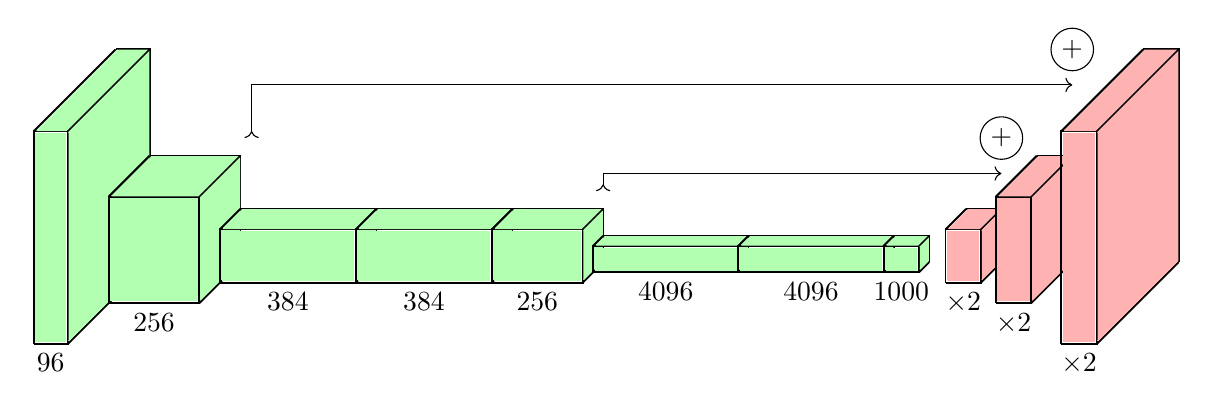
\begin{tikzpicture}[scale=0.9]
  \networkLayer{3.0}{0.48}{0}{0.0}{color=green!30}{96}
  \networkLayer{1.5}{1.28}{0.48}{0.0}{color=green!30}{256}
  \networkLayer{0.75}{1.92}{1.76}{0.0}{color=green!30}{384}
  \networkLayer{0.75}{1.92}{3.68}{0.0}{color=green!30}{384}
  \networkLayer{0.75}{1.28}{5.60}{0.0}{color=green!30}{256}
  \networkLayer{0.37}{2.05}{6.88}{0.0}{color=green!30}{4096}
  \networkLayer{0.37}{2.05}{8.93}{0.0}{color=green!30}{4096}
  \networkLayer{0.37}{0.5}{10.98}{0.0}{color=green!30}{1000}

  \networkLayer{0.75}{0.5}{12}{0.0}{color=red!30}{$\times 2$}
  \networkLayer{1.5}{0.5}{13}{0.0}{color=red!30}{$\times 2$}
  \networkLayer{3}{0.5}{14.5}{0.0}{color=red!30}{$\times 2$}

  \draw [>->] (1.92,1.75) -- (1.92,2.5) -- (13.5,2.5);
  \draw [>->] (6.88,1) -- (6.88,1.25) -- (12.5,1.25);

  \draw (13.5,3) circle [radius=0.3] node {$+$};
  \draw (12.5,1.75) circle [radius=0.3] node {$+$};
\end{tikzpicture}
\caption[The VGG-16 network]{Basic VGG-16~\cite{simonyan2014vgg}
  network with modifications added from
  FCN~\cite{long2015fully}. Information from lower levels of the
  network summed to upsampled output of the tailing end of the
  network. The number of features is shown below each convolution.}
\label{fig:background:fcn}
\end{figure}

\subsection{Part Segmentation}

There have been also a few works that
extend semantic segmentation to part segmentation with perhaps the
most well-known being the Shape Boltzman Machine
\cite{eslami2012generative,eslami2014shape}. This work has been
recently extended to incorporate CNN refined by CRF features (as in
\cite{chen2015semantic}) in \cite{tsogkas2015deep}. Note that this
work aims to refine the CNN output by applying a Restricted Boltzmann
Machine on top of it and does not make use of pose information as
provided by landmarks. In contrast, we propose an enhanced CNN
architecture which is landmark-guided, can be trained end-to-end and
yields large performance improvement without the need of further
refinement.


\subsection{Facial Part Segmentation}

One of the first face segmentation methods
prior to deep learning is known as LabelFaces
\cite{warrell2009labelfaces} which is based on patch classification
and further refinement via a hierarchical face model. Another
hierarchical approach to face segmentation based on Restricted
Boltzmann Machines was proposed in \cite{luo2012hierarchical}. More
recently, a multi-objective CNN has been shown to perform well for the
task of face segmentation in \cite{liu2015multi}. The method is based
on a CRF the unary and pairwise potentials of which are learnt via a
CNN. Softmax loss is used for the segmentation masks, and a logistic
loss is used to learn the edges. Additionally, the network makes use
of a non-parametric segmentation prior which is obtained as follows:
first facial landmarks on the test image are detected and then all
training images with most similar shapes are used to calculate an
average segmentation mask. This mask is finally used to augment
RGB. This segmentation mask might be blurry, does not encode pose
information and results in little performance improvement.











%%% Local Variables:
%%% TeX-master: "../thesis"
%%% End:
 % Literature Review
\graphicspath{{chapter_seg/}}
\chapter{A CNN Cascade for Landmark Guided Semantic Part Segmentation}

% \begin{abstract}
%   This paper proposes a CNN cascade for semantic part segmentation
%   guided by pose-specific information encoded in terms of a set of
%   landmarks (or keypoints). There is large amount of prior work on
%   each of these tasks separately, yet, to the best of our knowledge,
%   this is the first time in literature that the interplay between pose
%   estimation and semantic part segmentation is investigated. To
%   address this limitation of prior work, in this paper, we propose a
%   CNN cascade of tasks that firstly performs landmark localisation and
%   then uses this information as input for guiding semantic part
%   segmentation. We applied our architecture to the problem of facial
%   part segmentation and report large performance improvement over the
%   standard unguided network on the most challenging face
%   datasets. Testing code and models will be published online at
%   \url{http://cs.nott.ac.uk/~psxasj/}.  \keywords{pose estimation,
%     landmark localisation, semantic part segmentation, faces}
% \end{abstract}


\section{Introduction}

Pose estimation refers to the task of localising a set of landmarks
(or keypoints) on objects of interest like faces
\cite{cootes2001active}, the human body \cite{yang2011articulated} or
even birds \cite{zhang2015fine}. Locating these landmarks help
establish correspondences between two or more different instances of
the same object class which in turn has been proven useful for
fined-grained recognition tasks like face and activity
recognition. Part segmentation is a special case of semantic image
segmentation which is the task of assigning an object class label to
each pixel in the image. In part segmentation, the assigned label
corresponds to the part of the object that this pixel belongs to. In
this paper, we investigate whether pose estimation can guide
contemporary CNN architectures for semantic part segmentation. This
seems to be natural yet to the best of our knowledge this is the first
paper that addresses this problem. To this end, we propose a
Convolutional Neural Network (CNN) cascade for landmark guided part
segmentation and report large performance improvement over a standard
CNN for semantic segmentation that was trained without guidance.

Although the ideas and methods presented in this paper can probably be
applied to any structured deformable object (e.g. faces, human body,
cars, birds), we will confine ourselves to human faces. The main
reason for this is the lack of annotated datasets. To the best of our
knowledge, there are no datasets providing pixel-level annotation of
parts and landmarks at the same time. While this is also true for the
case of human faces, one can come up with pixel-level annotation of
facial parts by just appropriately connecting a pseudo-dense set of
facial landmarks for which many datasets and a very large number of
annotated facial images exist, see for example
\cite{sagonas2013semi}. Note that during testing we do not assume
knowledge of the landmarks' location, and what we actually show is
that a two-step process in which a CNN firstly predicts the landmarks
and then uses this information to segment the face largely outperforms
a CNN that was trained to directly perform facial part segmentation.

\begin{figure}
\centering
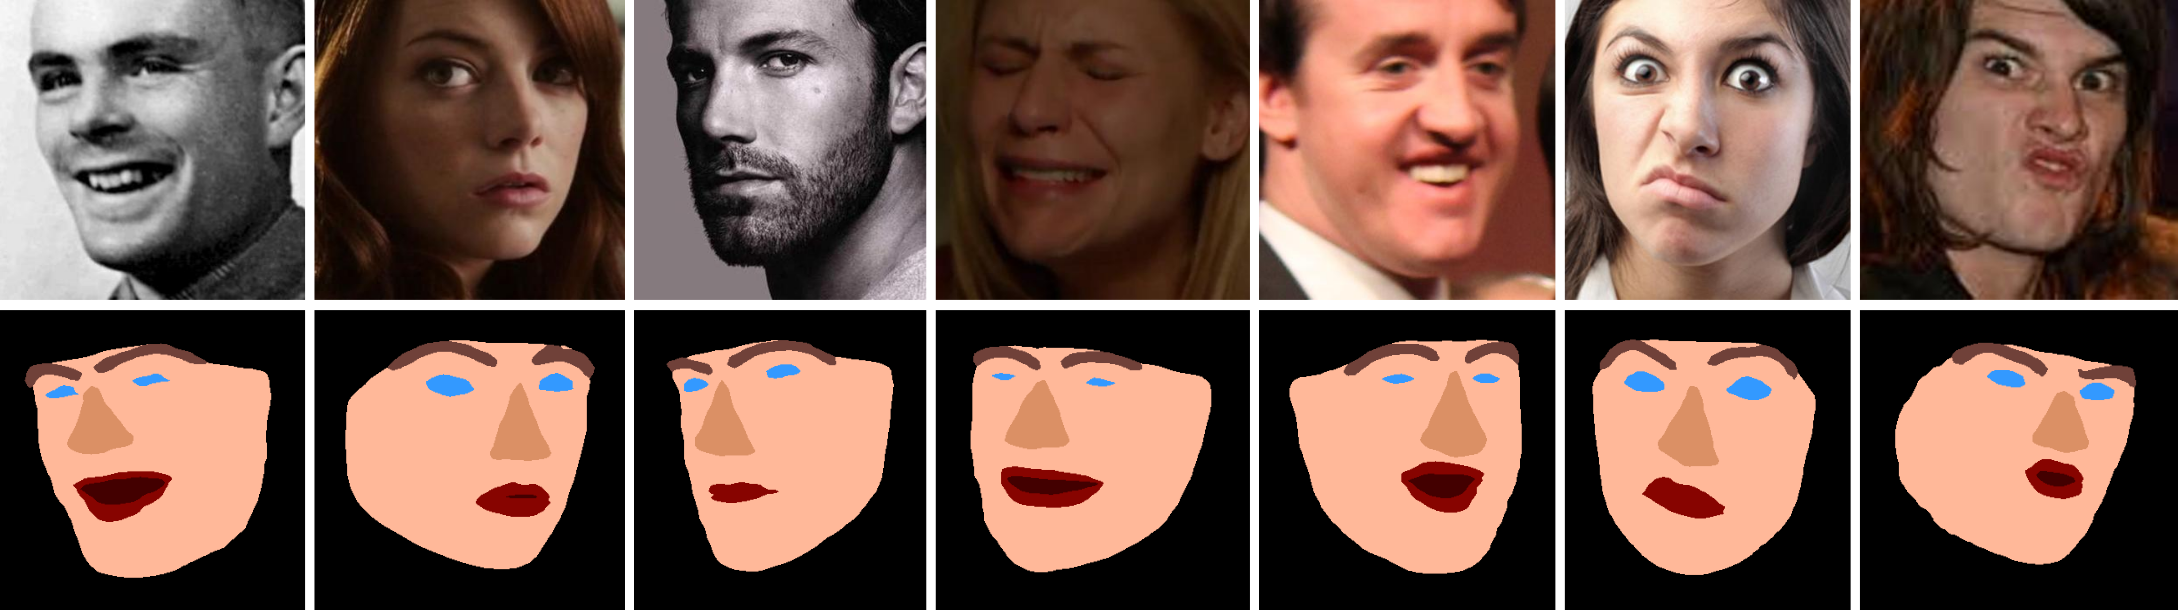
\includegraphics[width=\linewidth]{figs/sampler.png}
\caption{Examples from our facial part segmentation method}{Example
  faces and their corresponding output from the CNN cascade.}
\label{fig:sampler}
\end{figure}


\subsection{Main contributions}

In summary, this paper addresses the following research questions:
\begin{enumerate}
\item Is a CNN for facial part segmentation needed at all? One might
  argue that by just predicting the facial landmarks and then
  connecting them in the same way as we created the part labels, we
  could get high quality facial part segmentation thus completely
  by-passing the part segmentation task. Our first result in this
  paper is that indeed the latter method slightly outperforms a CNN
  trained for facial part segmentation (without guidance though).
\item Can facial landmarks be used for guiding facial part
  segmentation, thus reversing the result mentioned above? Indeed, we
  show that the proposed CNN cascade for landmark guided facial part
  segmentation largely outperforms both methods mentioned above
  without even requiring very accurate localisation of the
  landmarks. Some example output can be seen in Fig~\ref{fig:sampler}.
\end{enumerate}

\section{Related work}

This section reviews related work on semantic segmentation, facial
landmark localisation (also known as alignment) and facial part
segmentation.

\textbf{Face Alignment} State-of-the-art techniques in face alignment
are based on the so-called cascaded regression
\cite{dollar2010cascaded}. Given a facial image, such methods estimate
the landmarks' location by applying a sequence of regressors usually
learnt from SIFT \cite{lowe2004distinctive} or other hand-crafted
features. The regressors are learnt in a cascaded manner such that the
input to regressor $k$ is the estimate of the landmarks' location
provided by regressor $k-1$, see also
\cite{sanchez16,Cao2012shaperegression,xiongsupervised,zhu2015face,tzimiropoulos2015project}. The
first component in the proposed CNN cascade is a CNN landmark detector
based on VGG-16 \cite{simonyan2014very} converted to a fully
convolutional network \cite{long2015fully}. Although the main
contribution of our paper is not to propose a method for landmark
localisation, our CNN landmark localisation method performs comparably
with all aforementioned methods. One advantage of our method over
cascaded regression approaches is that it is not sensitive to
initialisation and hence it does not rely on accurate face detection.

\textbf{Semantic Segmentation} Thanks to its ability to integrate
information from multiple CNN layers and its end-to-end training, the
Fully Convolutional Network (FCN) of \cite{long2015fully} has become
the standard basic component for all contemporary semantic
segmentation algorithms. The architecture of FCN is shown in
Fig. \ref{fig:fcn}. One of the limitations of the FCN is that
prediction is performed in low-resolution, hence a number of methods
have been recently proposed to compensate for this by usually applying
a Conditional Random Field (CRF) on top of the FCN output. The work of
\cite{chen2015semantic} firstly upsamples the predicted scores using
bilinear interpolation and then refines the output by applying a dense
CRF. The method of \cite{zheng2015conditional} performs recurrent
end-to-end training of the FCN and the dense CRF. Finally, the work in
\cite{noh2015learning} employs learnt deconvolution layers, as opposed
to fixing the parameters with an interpolation filter (as in
FCN). These filters learn to reconstruct the object's shape, instead
of just classifying each pixel. Although any of these methods could be
incorporated within the proposed CNN cascade, for simplicity, we used
the VGG-FCN \cite{simonyan2014very}. Note that all the aforementioned
methods perform unguided semantic segmentation, as opposed to the
proposed landmark-guided segmentation which incorporates information
about the pose of the object during both training and testing. To
encode pose specific information we augment the input to our
segmentation network with a multi-channel confidence map
representation using Gaussians centred at the predicted landmarks'
location, inspired by the human pose estimation method of
\cite{carreira2016human}. Note that \cite{carreira2016human} is
iterative an idea that could be also applied to our method, but
currently we have not observed performance improvement by doing so.

\textbf{Part Segmentation} There have been also a few works that
extend semantic segmentation to part segmentation with perhaps the
most well-known being the Shape Boltzman Machine
\cite{eslami2012generative,eslami2014shape}. This work has been
recently extended to incorporate CNN refined by CRF features (as in
\cite{chen2015semantic}) in \cite{tsogkas2015deep}. Note that this
work aims to refine the CNN output by applying a Restricted Boltzmann
Machine on top of it and does not make use of pose information as
provided by landmarks. In contrast, we propose an enhanced CNN
architecture which is landmark-guided, can be trained end-to-end and
yields large performance improvement without the need of further
refinement.

\textbf{Face Segmentation} One of the first face segmentation methods
prior to deep learning is known as LabelFaces
\cite{warrell2009labelfaces} which is based on patch classification
and further refinement via a hierarchical face model. Another
hierarchical approach to face segmentation based on Restricted
Boltzmann Machines was proposed in \cite{luo2012hierarchical}. More
recently, a multi-objective CNN has been shown to perform well for the
task of face segmentation in \cite{liu2015multi}. The method is based
on a CRF the unary and pairwise potentials of which are learnt via a
CNN. Softmax loss is used for the segmentation masks, and a logistic
loss is used to learn the edges. Additionally, the network makes use
of a non-parametric segmentation prior which is obtained as follows:
first facial landmarks on the test image are detected and then all
training images with most similar shapes are used to calculate an
average segmentation mask. This mask is finally used to augment
RGB. This segmentation mask might be blurry, does not encode pose
information and results in little performance improvement.




% accepts input of arbitrary size, and through layers of convolution
% the input is reduced to a deep of feature matrix. This is scored
% (per-pixel classification) and upsampled, rendering an unrefined but
% globally aware segmentation mask. To refine this, lower level
% (local) information is scored and incorporated. %% FCN

% An alternative approach to incorporating local information was
% demonstrated in~\cite{hariharan2015hypercolumns}. The output of each
% convolution is upsampled to the original input size. This allows a
% feature vector to be formed for each pixel, which can be used for
% labelling. To better capture the finer details of an image,
% \cite{noh2015learning} employs learnt deconvolution layers, as
% opposed to fixing the parameters with an interpolation filter, as in
% FCN. These filters learn to reconstruct the object's shape, instead
% of just classifying each pixel.




% Semantic Segmentation Guided by Detected Boundaries However... this
% is a bit boring because it seems they use it to mask the
% segmentation masks at the end? As opposed to what we do, which is
% pass this information to the network in the first conv layer.
% https://www.semanticscholar.org/paper/Object-Boundary-Guided-Semantic-Segmentation-Huang-Xia/79a3a2960945dcee46d0bb29944f4d7d1a97f37b/pdf

\begin{figure}
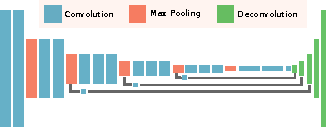
\includegraphics[width=\linewidth]{figs/FCN.pdf}
\caption{VGG-16 Network}{Overview of the
  Fully Convolutional Network~\cite{long2015fully}, low level
  information providing refinement are reintroduced into the network
  during deconvolution.}
\label{fig:fcn}
\end{figure}

\section{Datasets}
\label{sec:dataset}

There are a few datasets which provide annotations of pixel-level
parts \cite{bo2011shape,kae2013augmenting,chen2014detect} but to the
best of our knowledge there are no datasets containing both part and
landmark annotations. Hence, in our paper we rely on datasets for
facial landmarking. These datasets provide a pseudo-dense set of
landmarks. Segmentation masks are constructed by joining the
groundtruth landmarks together to fully enclose each facial
component. The eyebrows are generated by a spline with a fixed width
relative to the normalised face size, to cover the entire eyebrow. The
selected classes are background, skin, eyebrows, eyes, nose, upper
lip, inner mouth and lower lip. While this results in straight edges
between landmarks, the network can learn a mean boundary for each
class. The output from the network will be actually smoother than the
groundtruth.

This process is illustrated in Fig.~\ref{fig:gtmasks}.

\begin{figure}
\centering
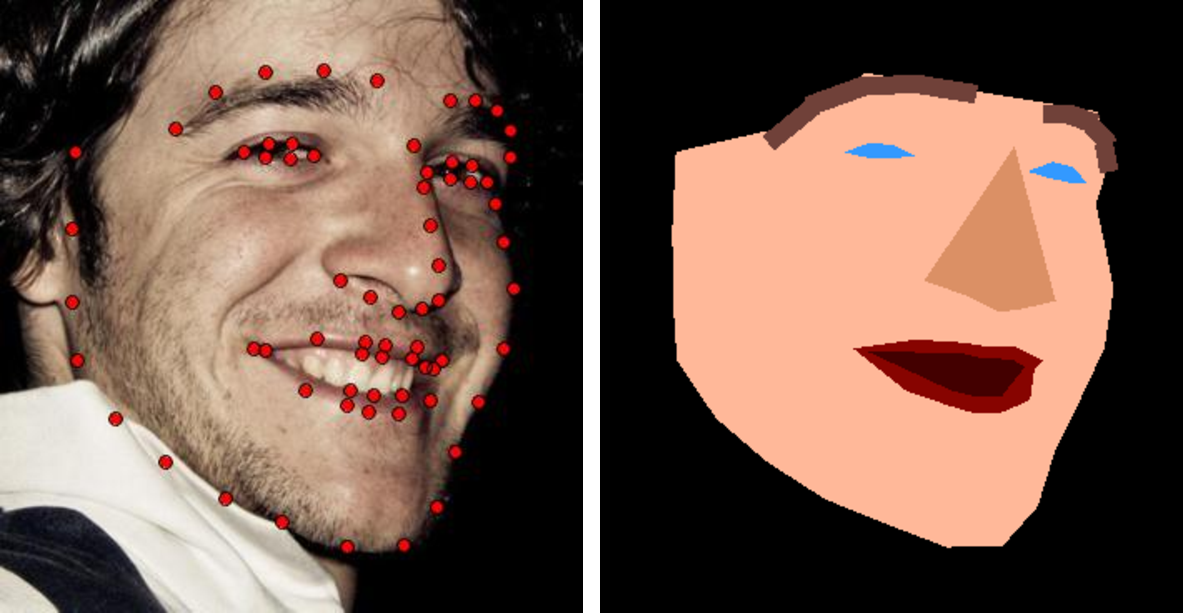
\includegraphics[height=3.5cm]{figs/gtmasks.pdf}
\hspace{-1.4mm}
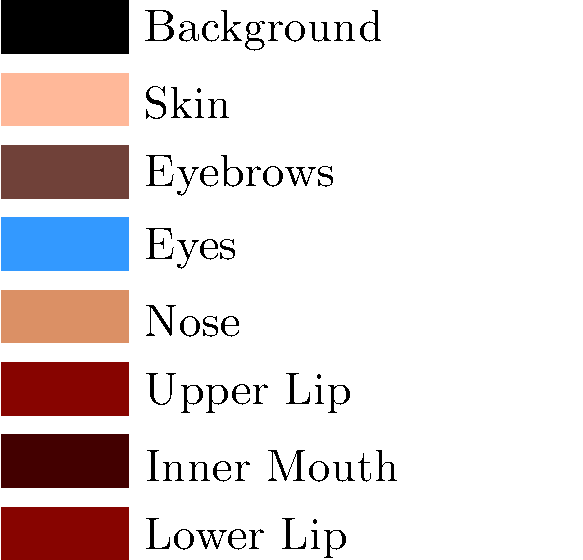
\includegraphics[height=3.5cm]{figs/gtmasks_key.pdf}
\caption{Example groundtruth facial part masks}{Example groundtruth
  segmentation mask produced from the groundtruth landmarks.}
\label{fig:gtmasks}
\end{figure}

For our experiments we used the 68-point landmark annotations provided
by the 300W challenge \cite{sagonas2013300}. In particular the
training sets of LFPW \cite{belhumeur2011localizing}, Helen
\cite{le2012interactive}, AFW \cite{ramanan2011} and iBUG
\cite{sagonas2013300} are all used for training while the 300W test
set (600 images) is used for testing. Both training and test sets
contain very challenging images in terms of appearance, pose,
expression and occlusion.

This collection of images undergoes some pre-processing before they
are used to train the network. The faces are normalised to be of equal
size and cropped with some noise added to the position of the bounding
box. Not all images are the same size, but their height is fixed at
350 pixels. With probability $p=0.5$, a randomly sized black
rectangle, large enough to occlude an entire component is layered over
the input image. This assists the network in learning a robustness to
partial occlusion.



\section{Method}
\label{sec:proposed}


\begin{figure}
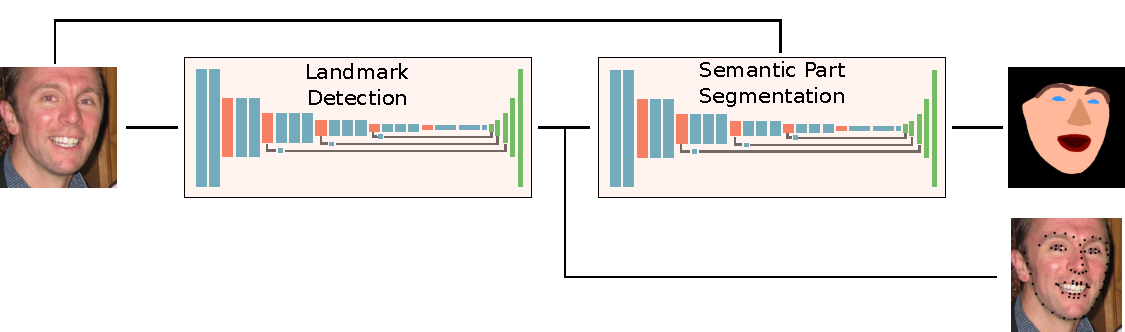
\includegraphics[width=\linewidth]{figs/Proposed.pdf}
\caption{Our proposed end-to-end architecture for facial part
  segmentation}{The proposed architecture, comprising of two separate
  Fully Convolutional Networks. The first performs Landmark Detection,
  the output of which is encoded as multichannel representation which
  is then passed into the Semantic Part Segmentation network.}
\label{fig:proposed}
\end{figure}

We propose a CNN cascade (shown in Fig.~\ref{fig:proposed} and listed
in Table~\ref{tab:archlist}) which performs landmark localisation
followed by facial part segmentation. Our cascade was based on the
VGG-FCN \cite{simonyan2014very,long2015fully} using Caffe
\cite{jia2014caffe} and consists of two main components:
\begin{enumerate}
\item Firstly, an FCN is trained to detect facial landmarks using
  Sigmoid Cross Entropy Loss.
\item Secondly, inspired by the human pose estimation method of
  \cite{carreira2016human}, the detected 68 landmarks are encoded as
  68 separate channels each of which contains a 2D Gaussian centred
  at the corresponding landmark's location. The 68 channels are then
  stacked along with the original image and passed into our
  segmentation network. This is a second FCN trained for facial part
  segmentation using as input the stacked representation of 2D
  Gaussians and image, and a standard Softmax loss.
\end{enumerate}

Overall we encode pose specific information by augmenting the input to
our segmentation network with a multi-channel confidence map
representation using Gaussians centred at the predicted landmarks'
location. Hence, our FCN for semantic segmentation is trained to
produce high quality, refined semantic masks by incorporating low
level information with globally aware information. Each of the
aforementioned components is now discussed in more detail:

% Training FCN for unguided part segmentation
% % learning rate, momentum, number of iterations, training steps
% % chosen loss
% Training FCN for landmark localisation
% % learning rate, momentum, number of iterations, training steps,
% % chosen loss
\textbf{Facial Landmark Detection} The training procedure for landmark
detection is similar to training FCN for part segmentation. Landmarks
are encoded as 2D Gaussians centred at the provided landmarks'
location. Each landmark is allocated its own channel to prevent
overlapping with other landmarks and allow the network to more easily
distinguish between each point. The main difference with part
segmentation is the loss function. Sigmoid Cross Entropy Loss
\cite{zhang2015fine} was chosen to regress the likelihood of a pixel
containing a point. More concretely, given our groundtruth Gaussians
$\hat{p}$ and predicted Gaussians $p$, each of equal dimensions
$ N \times W \times H$, we can define the Sigmoid Cross Entropy loss
$l$ as follows:

\[
  l = \frac{1}{N} \sum^{N}_{n=1} \sum^{W}_{i=1} \sum^{H}_{j=1}
  [p^n_{i,j} \log(\hat{p}^n_{i,j}) + (1 -p^n_{i,j})
  \log (1-\hat{p}^n_{i,j}) ].
\]

The loss was scaled by $1\mathrm{e}^{-5}$ and a learning rate of
0.0001 was used. The network was trained in steps as previously
described, for approximately 400,000 iterations, until convergence.


% Finetuning part segmentation to become guided
\textbf{Guided Facial Part Segmentation} To train our guided FCN part
segmentation network we followed \cite{long2015fully}. Softmax Loss
was also used. If $N$ is the number of outputs (in our case, classes),
$p_{i,j}$ is the predicted output for pixel $(i,j)$, and $n$ is the
true label for pixel $(i,j)$, then the Softmax loss $l$ can be defined
as:

% \[
% l = \frac{-1}{N} \sum^{N}_{n=1} \log ( p^{n}_{i,j} )
% \]

\[
l = \frac{-1}{N} \sum^{W}_{i=1} \sum^{H}_{j=1} \log(p^n_{i,j}).
\]

We firstly trained an unguided FCN for facial part segmentation
following \cite{long2015fully}. Initially, the network was trained as
32 stride, where no information from the lower layers is used to
refine the output. This followed by introducing information from
pool4, followed by pool3. A learning rate of 0.0001 was chosen, and a
momentum of 0.9. The network was trained for approximately 300,000
iterations until convergence.

Then, our guided FCN was initialised from the weights of the unguided
one, by expanding the first layer to accommodate the additional 68
input channels. As mentioned earlier, each channel contains a 2D
Gaussian centred at the corresponding landmark's location.  A key
aspect of our cascade is how the landmarks' location is determined
during training. We cannot use the groundtruth landmark locations nor
the prediction of our facial landmark detection network on our
training set as those will be significantly more accurate than those
observed during testing. Hence, we applied our facial landmark
detection network on our validation set and recorded the landmark
localisation error. We used this error to create a multivariate
Gaussian noise model that was added to the groundtruth landmark
locations of our training set. This way our guided segmentation
network was initialised with much more realistic input in terms of
landmarks' location. Furthermore, the same learning rate of 0.0001 was
used. For the first 10,000 iterations, training was disabled on all
layers except for the first. This allowed the network to warm up
slightly, and prevent the parameters in other layers from getting
destroyed by a high loss.

\begin{table}
  \caption{The
    VGG-FCN~\cite{simonyan2014very,long2015fully}
    architecture employed by our landmark detection and semantic
    part segmentation network.}
\label{tab:archlist}
\centering
\begin{tabular}{|c|c|c|c|}
\hline
Layer Name           & Kernel       & Stride       &  Outputs  \\
\hline\hline
\texttt{conv1\_1}    & $3 \times 3$ & $1 \times 1$ &  64  \\
\texttt{conv1\_2}    & $3 \times 3$ & $1 \times 1$ &  64  \\
\texttt{pool1}       & $2 \times 2$ & $2 \times 2$ &  --  \\
\texttt{conv2\_1}    & $3 \times 3$ & $1 \times 1$ &  128 \\
\texttt{conv2\_2}    & $3 \times 3$ & $1 \times 1$ &  128 \\
\texttt{pool2}       & $2 \times 2$ & $2 \times 2$ &  --  \\
\texttt{conv3\_1}    & $3 \times 3$ & $1 \times 1$ &  256 \\
\texttt{conv3\_2}    & $3 \times 3$ & $1 \times 1$ &  256 \\
\texttt{conv3\_3}    & $3 \times 3$ & $1 \times 1$ &  256 \\
\texttt{pool3}       & $2 \times 2$ & $2 \times 2$ &  --  \\
\texttt{conv4\_1}    & $3 \times 3$ & $1 \times 1$ & 512  \\
\texttt{conv4\_2}    & $3 \times 3$ & $1 \times 1$ & 512  \\
\texttt{conv4\_3}    & $3 \times 3$ & $1 \times 1$ & 512  \\

\hline
\end{tabular}
\begin{tabular}{|c|c|c|c|}
\hline
Layer Name           & Kernel       & Stride       &  Outputs  \\
\hline\hline
\texttt{pool4}       & $2 \times 2$ & $2 \times 2$ & --   \\
\texttt{conv5\_1}    & $3 \times 3$ & $1 \times 1$ & 512  \\
\texttt{conv5\_2}    & $3 \times 3$ & $1 \times 1$ & 512  \\
\texttt{conv5\_3}    & $3 \times 3$ & $1 \times 1$ & 512  \\
\texttt{pool5}       & $2 \times 2$ & $2 \times 2$ & --   \\
\texttt{fc6\_conv}   & $7 \times 7$ & $1 \times 1$ & 4096 \\
\texttt{fc7\_conv}   & $1 \times 1$ & $1 \times 1$ & 4096 \\
\texttt{fc8\_conv}   & $1 \times 1$ & $1 \times 1$ & 68 or 7 \\
\texttt{deconv\_32}   & $4 \times 4$ & $2 \times 2$ & 68 or 7 \\
\texttt{score\_pool4} & $1 \times 1$ & $1 \times 1$ & 68 or 7 \\
\texttt{deconv\_16}   & $4 \times 4$ & $2 \times 2$ & 68 or 7 \\
\texttt{score\_pool3} & $1 \times 1$ & $1 \times 1$ & 68 or 7 \\
\texttt{deconv\_8}    & $16 \times 16$ & $8 \times 8$ & 68 or 7 \\
\hline
\end{tabular}
\end{table}


\section{Experiments}

\subsection{Overview of Results}

In all experiments we used the training and test sets detailed in
Section \ref{sec:dataset}. As a performance measure, we used the
familiar intersection over union measure \cite{long2015fully}. We
report a comparison between the performance of four different methods
of interest:
\begin{enumerate}
\item The first method is the VGG-FCN trained for facial part
  segmentation. We call this method \textbf{Unguided}.
\item The second method is the part segmentation result obtained by
  joining the landmarks obtained from VGG-FCN trained for facial
  landmark detection. We call this method \textbf{Connected
    Landmarks}.
\item The third method is the proposed landmark guided part
  segmentation network where the input is the groundtruth landmarks'
  location. We call this method \textbf{Guided by Groundtruth}.
\item Finally, the fourth method is the proposed landmark guided part
  segmentation network when input is detected landmarks' location. We
  call this method \textbf{Guided by Detected}.
\end{enumerate}
The first two methods are the baselines in our experiments while the
third one provides an upper bound in performance. The fourth method is
the proposed CNN cascade.

% \subsection{Facial Part Segmentation from Detected Landmarks}

% In this experiment we attempt to show the performance of facial part
% segmentation by connecting the detected landmarks. Although
% groundtruth landmarks were used to generate the groundtruth
% segmentation masks for training, the quality of part segmentation by
% joining detected landmarks was quite disappointing.

\subsection{Unguided Facial Part Segmentation}

\begin{figure}
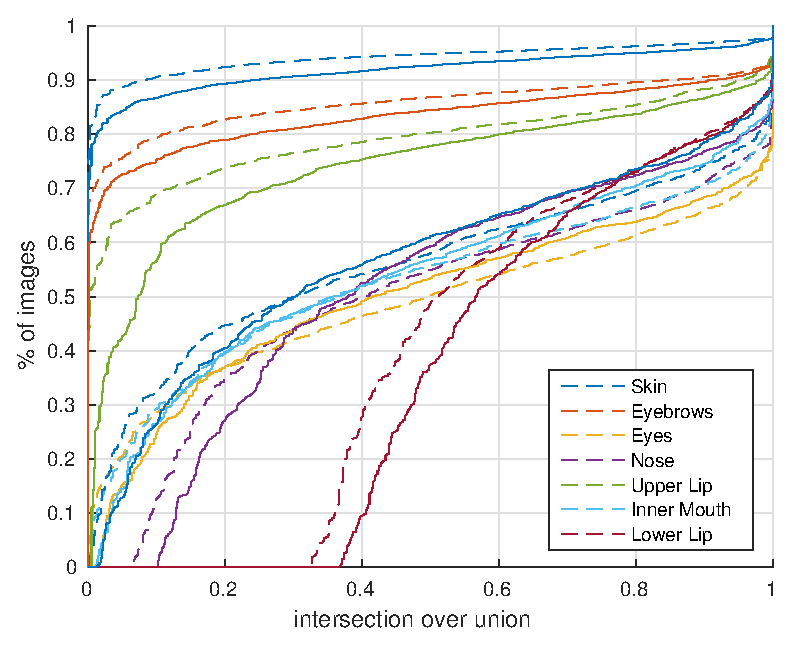
\includegraphics[width=0.5\linewidth]{figs/lan-vs-un.eps}
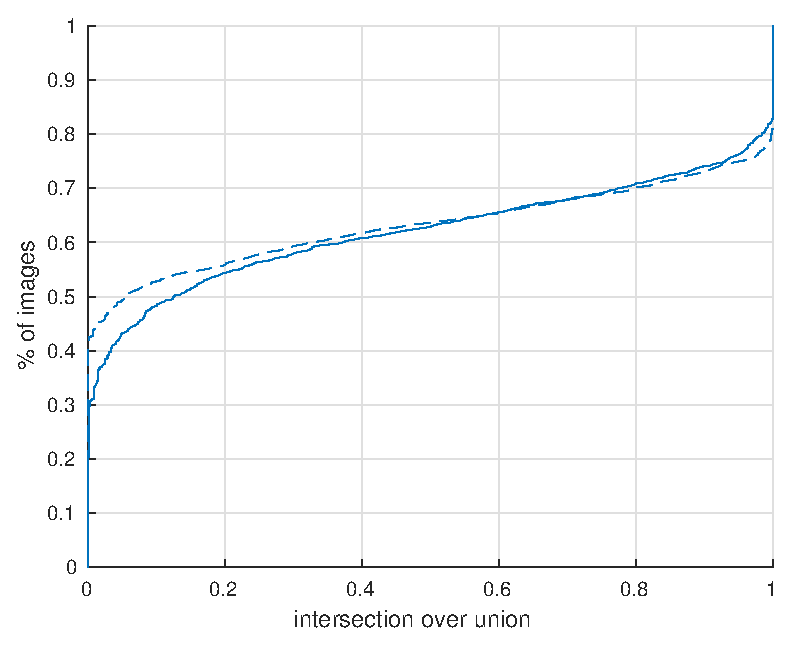
\includegraphics[width=0.5\linewidth]{figs/lan-vs-un-mean.eps}
\caption{Unguided vs. Guided facial part segmentation}{Comparison of
  Unguided (---) and Connected Landmarks (-{ }-). Per-class averages
  shown on the right.}
\label{fig:lan-vs-un}
\end{figure}

To establish a baseline, an unguided fully convolutional network was
firstly trained. This was done as described in the FCN paper
\cite{long2015fully} and Section \ref{sec:proposed}. Some visual
results can be seen in Fig.~\ref{fig:visual}. Additionally, a second
baseline was obtained by simply connecting the landmarks of our facial
landmark detection network also described in Section
\ref{sec:proposed}. The performance of both baselines can be seen in
Fig. \ref{fig:lan-vs-un}. We may observe that connecting the landmarks
appears to offer slightly better performance than FCN for part
segmentation alone. Nevertheless, we need to emphasise that the
groundtruth masks were obtained by connecting the landmarks and hence
there is some bias towards the connecting the landmarks approach.

\subsection{Guided Facial Part Segmentation with Groundtruth}

\begin{figure}
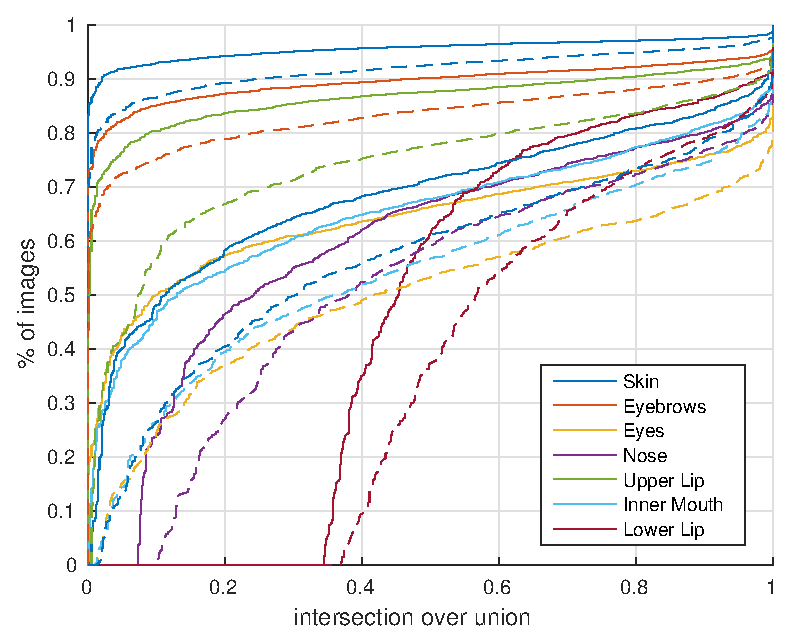
\includegraphics[width=0.5\linewidth]{figs/gtguided-vs-unguided.eps}
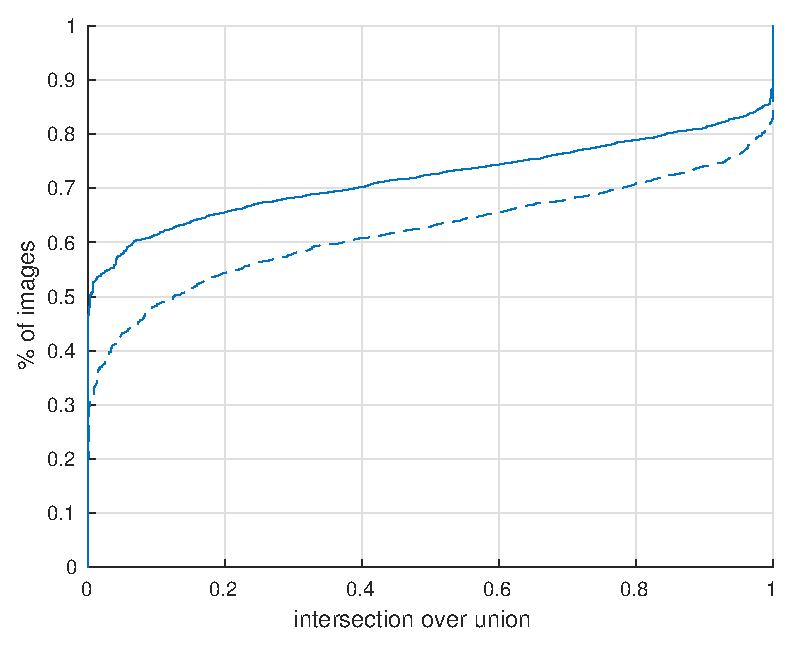
\includegraphics[width=0.5\linewidth]{figs/gtguided-vs-unguided-mean.eps}
\caption{Groundtruth Guided vs. Unguided facial part
  segmentation}{Comparison of guided by groundtruth (---) and unguided
  (-{ }-) facial part segmentation. Per-class averages shown on the
  right.  }
\label{fig:gt-vs-un}
\end{figure}

To establish an upper bounds to our performance, a fully convolutional
network was trained to accept guidance from groundtruth landmarks. As
described in Section~\ref{sec:proposed}, the guidance is provided in
the form of landmarks encoded as 2D Gaussians. The performance
difference between unguided and groundtruth guided part segmentation
can be seen in Fig.~\ref{fig:gt-vs-un}. As we may observe the
difference in performance between the two methods is huge. These
results are not surprising given that the groundtruth semantic masks
are generated from the landmarks guiding the network. Furthermore,
landmark detection offers an advantage because, in the case of faces,
there can only be one tip of the nose, and one left side of the
mouth. Giving some information to the network about where it is likely
to be located can offer a significant advantage. Our next experiment
shows that this is still the case when detected landmarks are used
instead of groundtruth landmarks.



\subsection{Guided Facial Part Segmentation with Detected Landmarks}

% Maybe this should be guidance by detected vs. unguided?
\begin{figure}
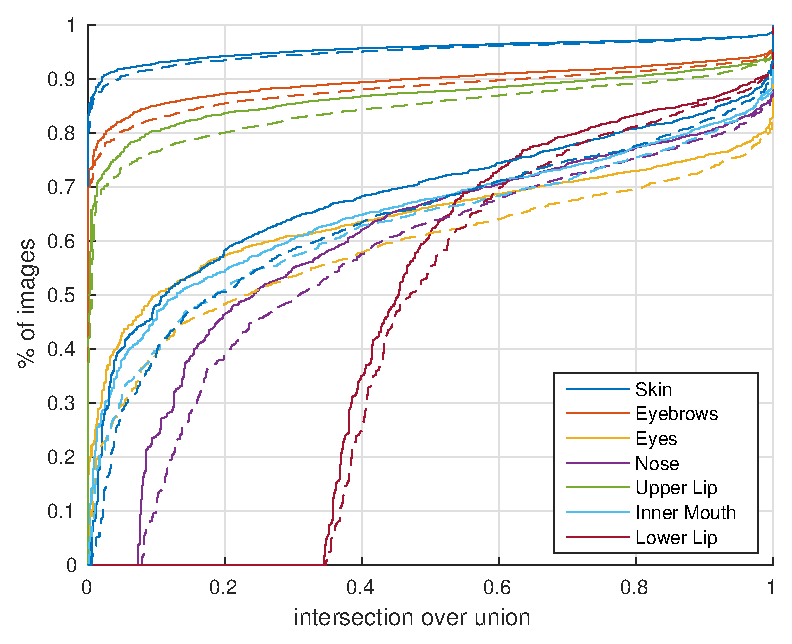
\includegraphics[width=0.5\linewidth]{figs/gtguided-vs-guided.eps}
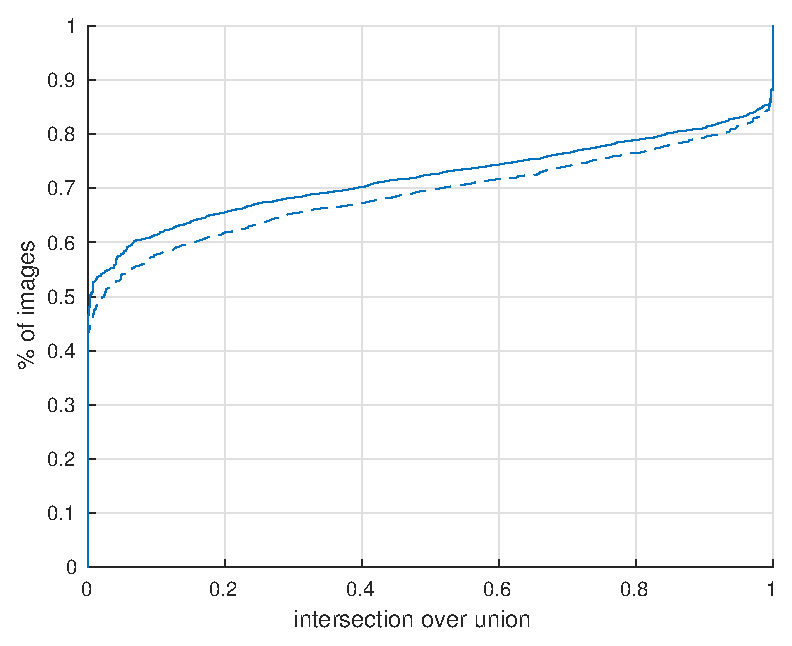
\includegraphics[width=0.5\linewidth]{figs/gtguided-vs-guided-mean.eps}
\caption{Groundtruth vs. Detected landmarks for guidance}{Comparison
  of guidance from groundtruth landmarks (---) and guidance from
  detected landmarks (-{ }-). Per-class averages shown on the right.
}
\label{fig:gt-vs-det}
\end{figure}

With our upper bound and baselines defined, we can now see how much of
an improvement we can achieve by guiding the network with our
detected landmarks. The output of the landmark detection network is
passed into the part segmentation network along with the original
input image. We acknowledge that the performance of our landmark
detector is far from groundtruth. We measure the performance as mean
point to point Euclidean distance normalised by the outer interocular
Euclidean distance, as in~\cite{sagonas2013300}. This results in an
error of $0.0479$. However, we show that the performance of the
segmentation is improved significantly. The results of facial part
segmentation guided by the detected landmarks, compared to the network
guided by groundtruth landmarks can be seen in
Fig~\ref{fig:gt-vs-det}. Our main result is that performance of the
guided by detected network is very close to the that of the guided by
groundtruth illustrating that in practice accurate landmark
localisation is not really required to guide segmentation. Some visual
results can be seen in Fig.~\ref{fig:visual}. Also, performance over
all components for all methods is given in Fig.~\ref{fig:all}.



\begin{figure}
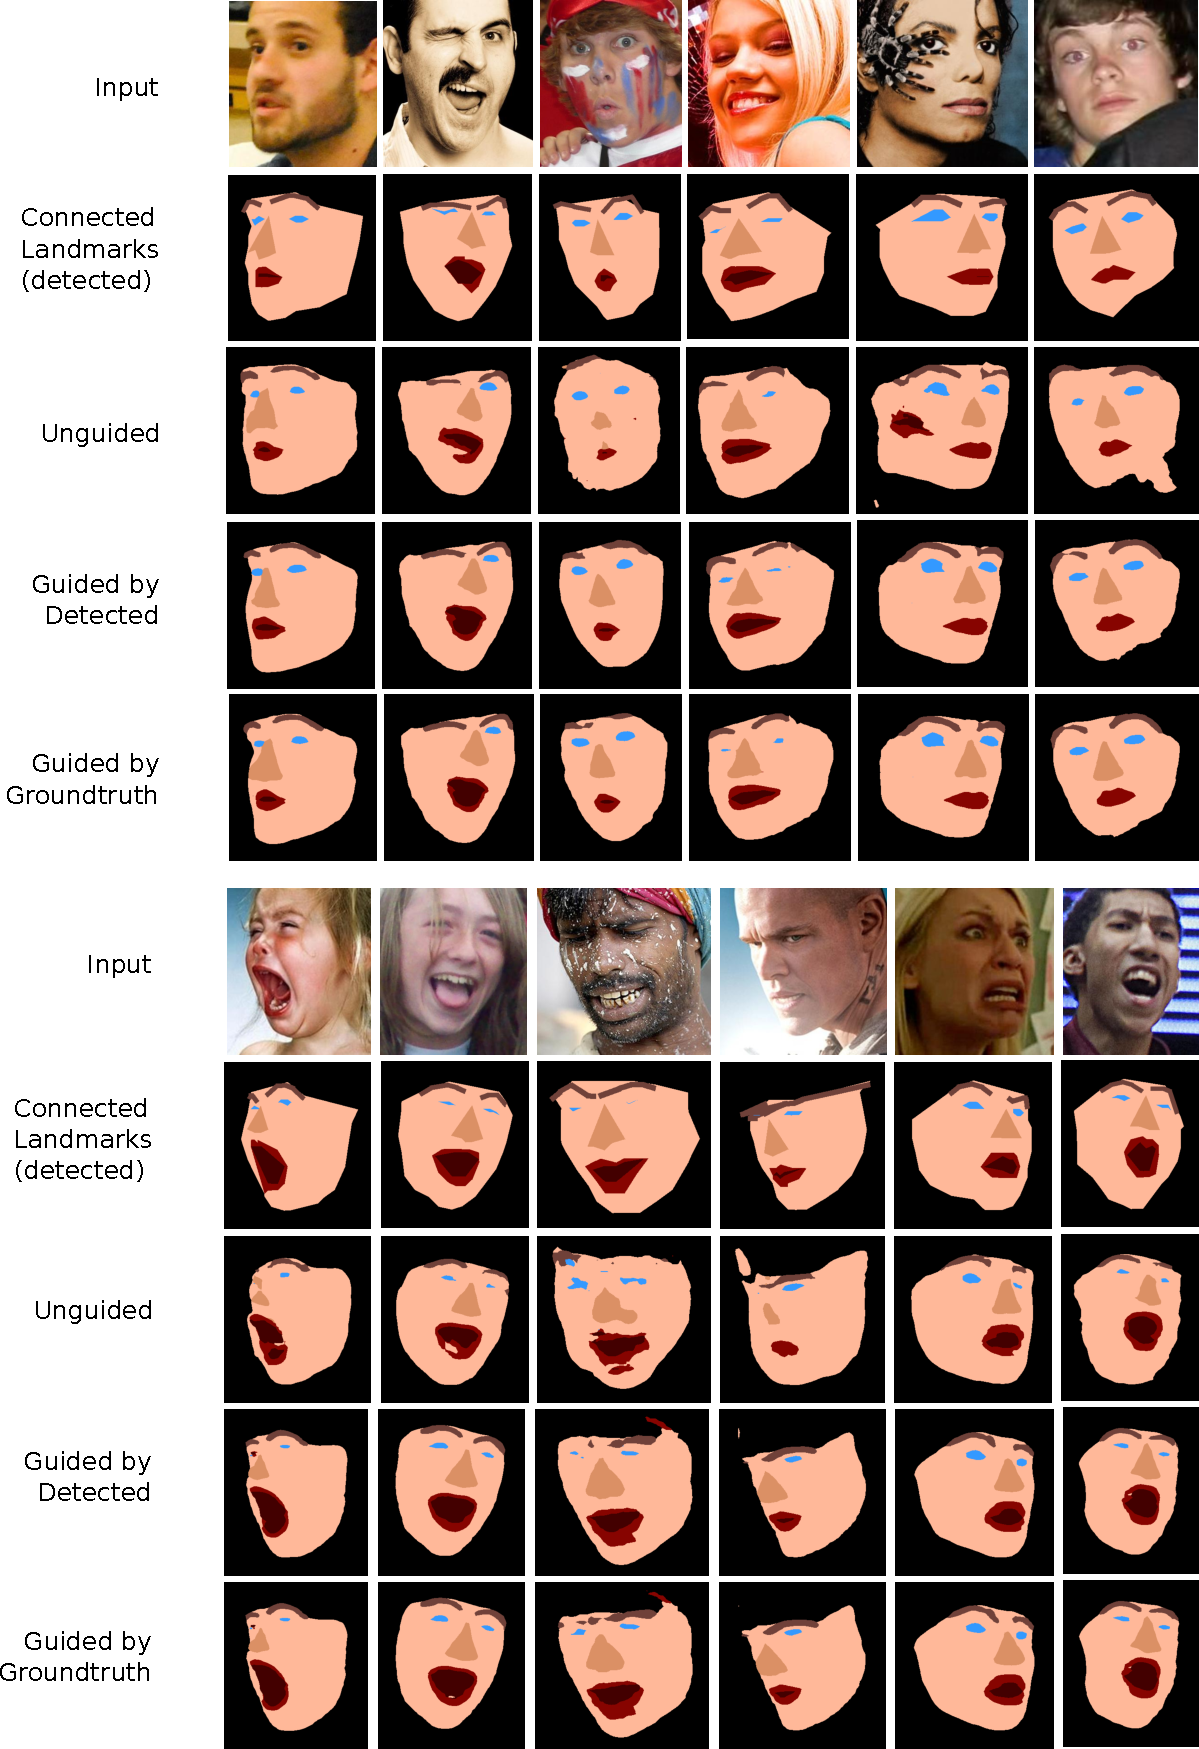
\includegraphics[width=\linewidth]{figs/Visual.pdf}
\caption{Challenging images and their output from facial part
  segmentation}{Some visual results showing where the unguided network
  begins to fail, and where the guidance begins to pay off. Observe
  how visually close the results of the guided by groundtruth
  landmarks and the guided by detected landmarks networks are.}
\label{fig:visual}
\end{figure}

\begin{figure}
\centering
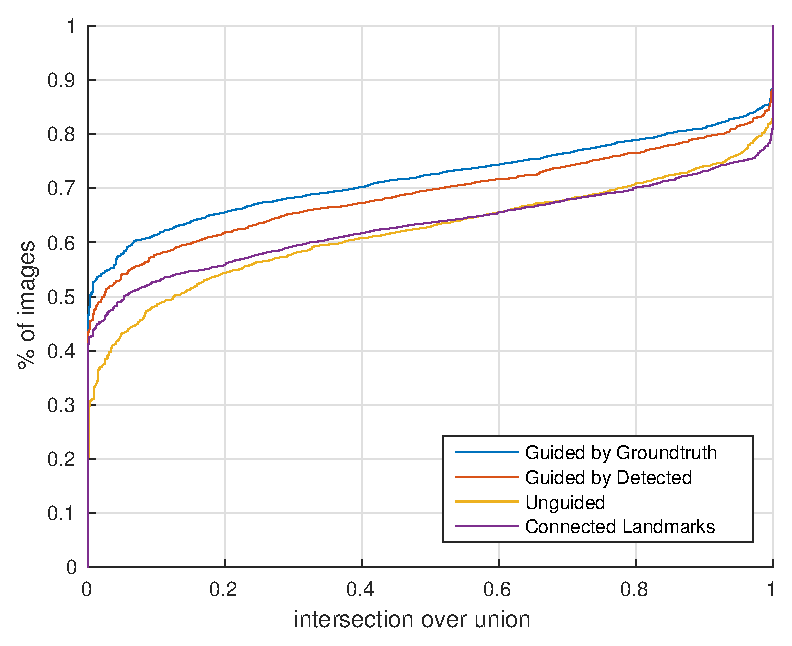
\includegraphics[width=0.6\linewidth]{figs/all.eps}
\caption{Average images and their output from facial part
  segmentation}{Average performance of the four tested methods over
  all facial components: part segmentation guided by groundtruth
  landmarks, part segmentation guided by detected landmarks, unguided
  part segmentation, part segmentation by joining up the detected
  landmarks.}
\label{fig:all}
\end{figure}


\section{Conclusion}

In this paper we proposed a CNN architecture to improve the
performance of part segmentation by task delegation. In doing so, we
provided both landmark localisation and semantic part segmentation on
human faces. However, our method should be applicable to our objects
as well. This is the focus of our ongoing work. We are also looking
into how the segmentation masks can be further used to improve
landmark localisation accuracy, thus leading to a recurrent
architecture. Future work may also compare the performance of this
method with a multitask architecture.

%%% Local Variables:
%%% TeX-master: "../thesis"
%%% End: % Facial Part Segmentation
\graphicspath{{chapter_faces/}}
\chapter{Large Pose 3D Face Reconstruction via Volumetric Regression}
\label{chapter:face}

\begin{figure}
  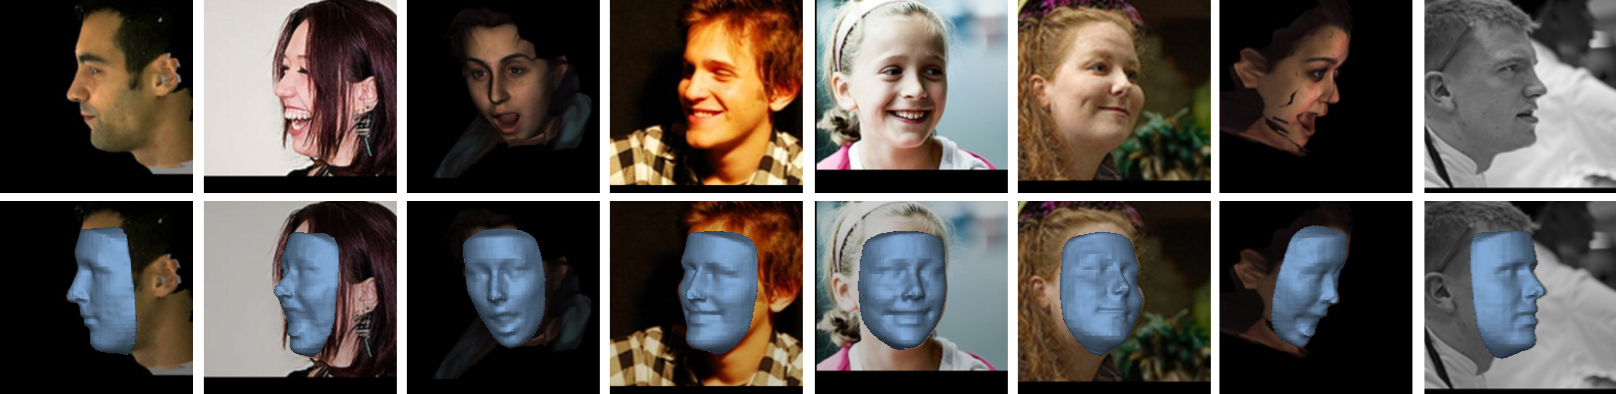
\includegraphics[width=\linewidth]{img/preview.png}
  \caption[A 3D Reconstruction Preview]{A preview of our 3D
    reconstruction method, applied on a wide variety of poses.}
  \label{c:face:fig:preview}
\end{figure}
% \begin{abstract}
%   3D face reconstruction is a fundamental Computer Vision problem of
%   extraordinary difficulty. Current systems often assume the
%   availability of multiple facial images (sometimes from the same
%   subject) as input, and must address a number of methodological
%   challenges such as establishing dense correspondences across large
%   facial poses, expressions, and non-uniform illumination. In general
%   these methods require complex and inefficient pipelines for model
%   building and fitting. In this work, we propose to address many of
%   these limitations by training a Convolutional Neural Network (CNN)
%   on an appropriate dataset consisting of 2D images and 3D facial
%   models or scans. Our CNN works with just a single 2D facial image,
%   does not require accurate alignment nor establishes dense
%   correspondence between images, works for arbitrary facial poses and
%   expressions, and can be used to reconstruct the whole 3D facial
%   geometry (including the non-visible parts of the face) bypassing the
%   construction (during training) and fitting (during testing) of a 3D
%   Morphable Model. We achieve this via a simple CNN architecture that
%   performs direct regression of a volumetric representation of the 3D
%   facial geometry from a single 2D image. We also demonstrate how the
%   related task of facial landmark localization can be incorporated
%   into the proposed framework and help improve reconstruction quality,
%   especially for the cases of large poses and facial
%   expressions. Code and models will be made available at \verb|http://aaronsplace.co.uk|
% \end{abstract}
% \vspace{-4mm}

3D face reconstruction is a fundamental Computer Vision problem, often
considered to be of extraordinary difficultly. Current systems often
assume the availability of multiple facial images as input, sometimes
from the same subject. Additional, there are a number of
methodological challenges involved, which must be addressed. These
challenges include establishing a dense correspondence across large
poses, expressions and non-uniform illumination. In general, these
methods require complex and inefficient pipelines for model building
and fitting. In this work, we propose to address many of these
limitations by constraining the problem of 3D face reconstruction to
the spatial domain. We do this by training a Convolutional Neural
Network (CNN), on an appropriate dataset, consisting of 2D images and
3D facial models, or scans. Our CNN works with just a single 2D facial
image and does not require accurate alignment. Our method works for
arbitrary facial poses and expressions, and can be used to
reconstruction the whole 3D facial geometry, including non-visible
parts. Our method bypasses the construction (during training) and
fitting (during inference) of a 3D Morphable Model. We achieve this via
a simple CNN architecture that performs direct regression of a
volumetric representation of the 3D facial geometry from a single 2D
image. We also demonstrate how the related task of facial landmark
localisation can be incorporated into the proposed framework and help
improve reconstruction quality, especially in the cases of large poses
and facial expressions.


\section{Introduction}
3D face reconstruction is the problem of recovering the 3D facial
geometry from 2D images. Despite many years of research, it is still
an open problem in Computer Vision and Graphics research. Depending on
the setting and the assumptions made, there are many variations of it,
as well as a multitude of approaches to solve it. This work is on 3D
face reconstruction using only a single image. Under this setting, the
problem is considered far from being solved. In this chapter, we
propose to approach it, for the first time to the best of our
knowledge, by directly learning a mapping from pixels to 3D
coordinates using a Convolutional Neural Network (CNN). Besides its
simplicity, our approach works with totally unconstrained images
downloaded from the web, including facial images of arbitrary poses,
facial expressions and occlusions, as shown in
Figure~\ref{c:face:fig:preview}. \newline \textbf{Motivation.} No
matter what the underlying assumptions are, what the input(s) and
output(s) to the algorithm are, 3D face reconstruction requires in
general complex pipelines and solving non-convex difficult
optimization problems for both model building (during training) and
model fitting (during testing). In the following paragraphs, we provide
examples from 5 predominant approaches:

\begin{enumerate}
\item In the 3D Morphable Model (3DMM) \cite{blanz1999morphable,
    romdhani2005estimating}, the most popular approach for estimating
  the full 3D facial structure from a single image (among others),
  training includes an iterative flow procedure for dense image
  correspondence which is prone to failure. Additionally, testing
  requires a careful initialisation for solving a difficult highly
  non-convex optimization problem in order to estimate the pose and
  shape parameters, which is slow.
\item The work of \cite{kemelmacher20113d}, a popular approach for
  2.5D reconstruction from a single image, formulates and solves a
  carefully initialised (for frontal images only) non-convex
  optimization problem for recovering the lighting, depth, and albedo
  in an alternating manner where each of the sub-problems is a
  difficult optimization problem per se.
\item In \cite{kemelmacher2011face}, a quite popular recent approach
  for creating a neutral subject-specific 2.5D model from a near
  frontal image, an iterative procedure is proposed which entails
  localising facial landmarks, face frontalization, solving a
  photometric stereo problem, local surface normal estimation, and
  finally shape integration.
\item In \cite{suwajanakorn2014total}, a state-of-the-art pipeline for
  reconstructing a highly detailed 2.5D facial shape for each video
  frame, an average shape and an illumination subspace for the
  specific person is firstly computed (offline), while testing is an
  iterative process requiring a sophisticated pose estimation
  algorithm, 3D flow computation between the model and the video
  frame, and finally shape refinement by solving a shape-from-shading
  optimization problem.
\item More recently, the state-of-the-art method of
  \cite{roth2016adaptive} that produces the average (neutral) 3D face
  from a collection of personal photos, firstly performs landmark
  detection, then fits a 3DMM using a sparse set of points, then
  solves an optimization problem similar to the one in
  \cite{kemelmacher2011face}, then performs surface normal estimation
  as in \cite{kemelmacher2011face} and finally performs surface
  reconstruction by solving another energy minimisation problem.
\end{enumerate}

Simplifying the technical challenges involved in the aforementioned
works is the main motivation of this work.

\subsection{Main contributions}
We describe a very simple approach which bypasses many of the
difficulties encountered in 3D face reconstruction by using a
novel volumetric representation of the 3D facial geometry, and
an appropriate CNN architecture that is trained to regress directly
from a 2D facial image to the corresponding 3D volume. An overview of
our method is shown in Figure~\ref{fig:cnnall}. In summary, our contributions
are:
\begin{itemize}
\item Given a dataset consisting of 2D images and 3D face scans, we
  investigate whether a CNN can learn directly, in an end-to-end
  fashion, the mapping from image pixels to the full 3D facial
  structure geometry (including the non-visible facial parts). Indeed,
  we show that the answer to this question is positive.
\item We demonstrate that our CNN works with just a single 2D facial
  image, does not require accurate alignment nor establishes dense
  correspondence between images, works for arbitrary facial poses and
  expressions, and can be used to reconstruct the whole 3D facial
  geometry bypassing the construction (during training) and fitting
  (during testing) of a 3DMM.
\item We achieve this via a simple CNN architecture that performs
  \textit{direct} regression of a volumetric representation of the 3D
  facial geometry from a single 2D image. 3DMM fitting is not
  used. Our method uses only 2D images as input to the proposed CNN
  architecture.
\item We show how the related task of 3D facial landmark localisation
  can be incorporated into the proposed framework and help improve
  reconstruction quality, especially for the cases of large poses and
  facial expressions.
\item We report results for a large number of experiments on both
  controlled and completely unconstrained images from the web,
  illustrating that our method outperforms prior work on single image
  3D face reconstruction by a large margin.
\end{itemize}

\section{Method}


This section describes our framework including the proposed data representation used.


\subsection{Dataset}

Our aim is to regress the full 3D facial structure from a 2D image. To
this end, our method requires an appropriate dataset consisting of 2D
images and 3D facial scans. As our target is to apply the method on
completely unconstrained images from the web, we chose the dataset of
\cite{zhu2016face} for forming our training and test sets. The dataset
has been produced by fitting a 3DMM built from the combination of the
Basel \cite{paysan20093d} and FaceWarehouse
\cite{cao2014facewarehouse} models to the unconstrained images of the
300W dataset \cite{sagonas2013semi} using the multi-feature fitting
approach of \cite{romdhani2005estimating}, careful initialisation and
by constraining the solution using a sparse set of landmarks. Face
profiling is then used to render each image to 10-15 different poses
resulting in a large scale dataset (more than 60,000 2D facial images
and 3D meshes) called 300W-LP. Each mesh consists of approximately
53000 vertices, enclosing the face entirely. However, no vertices
exist around the mouth, base of neck and eyes, and as such, this mesh
is not watertight. All images are $450 \times 450$, although these are
downsampled to $386 \times 386$ during training. Note that because
each mesh is produced by a 3DMM, the vertices of all produced meshes
are in dense correspondence; however this is not a prerequisite for
our method and unregistered raw facial scans could be also used if
available (e.g. the BU-4DFE dataset~\cite{yin2008high}).

\subsection{Proposed volumetric representation}

Our goal is to predict the coordinates of the 3D vertices of each
facial scan from the corresponding 2D image via CNN regression. As a
number of works have pointed out (see for example
\cite{tompson2015efficient, pfister2015flowing}), direct regression of
all 3D points concatenated as a vector using the standard L2 loss
might cause difficulties in learning because a single correct value
for each 3D vertex must be predicted. Additionally, such an approach
requires interpolating all scans to a vector of a fixed dimension, a
pre-processing step not required by our method. Note that similar
learning problems are encountered when a CNN is used to regress model
parameters like the 3DMM parameters rather than the actual
vertices. In this case, special care must be taken to weight
parameters appropriately using the Mahalanobis distance or in general
some normalisation method, see for example \cite{zhu2016face}. We
compare the performance of our method with that of a similar
method~\cite{zhu2016face} in Section~\ref{S:Results}.

\begin{figure}
  \centering
  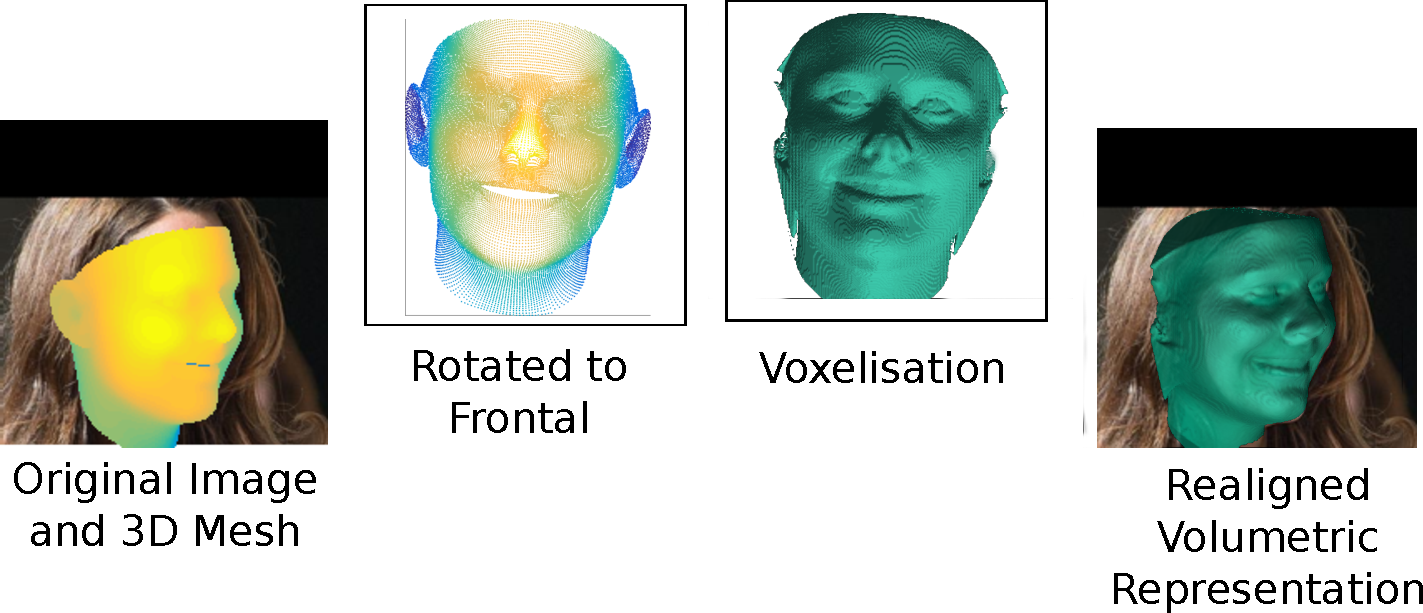
\includegraphics[width=0.9\linewidth]{img/discretisation.pdf}

  \caption[Dataset voxelisation procedure]{The voxelisation process
    creates a volumetric representation of the 3D face mesh, aligned
    with the 2D image.}
  \label{fig:discretisation}
\end{figure}

% Is it reasonable to say 2D to 3D image segmentation?
To alleviate the aforementioned learning problem, we propose to
reformulate the problem of 3D face reconstruction as one of 2D to 3D
image segmentation: in particular, we convert each 3D facial scan into
a 3D binary volume $\mathbf{V}_{whd}$ by discretizing the 3D space
into voxels $\{w,h,d\}$, assigning a value of 1 to all points enclosed
by the 3D facial scan, and 0 otherwise. That is to say $ V_{whd}$ is
the ground truth for voxel $\{w,h,d\}$ and is equal to 1, if voxel
$\{w,h,d\}$ belongs to the 3D volumetric representation of the face
and 0 otherwise (i.e. it belongs to the background). The conversion is
shown in Figure~\ref{fig:discretisation}. Contrary to standard
approaches, this data was voxelised by rotating to frontal and
estimating a depth map is estimated using bilinear interpolation. from
which the volume is filled back to a fixed point. This results in the
mouth becoming filled. Notice that the process creates a volume fully
aligned with the 2D image. The importance of spatial alignment is
analysed in more detail in Section~\ref{sec:spatialimportance}. The
error caused by discretization for a randomly picked facial scan as a
function of the volume size is shown in
Figure~\ref{fig:voxerror}. Given that the error of state-of-the-art
methods \cite{roth2016adaptive,liu2016joint} is of the order of a few
mms, we conclude that discretization by $192\times 192\times 200$
produces negligible error. Such a spatial resolution is ideal for the
type of architecture we have chosen to use as it can be reduced by
half many times. The depth, 200, was chosen to capture as much depth
information as possible without sacrificing the spatial resolution or
increasing the memory requirements too much.

Given our volumetric facial representation, the problem of regressing
the 3D coordinates of all vertices of a facial scan is reduced to one
of 3D binary volume segmentation. We approach this problem using
recent CNN architectures from semantic image segmentation
\cite{long2015fully} and their extensions \cite{newell2016stacked}, as
described in the next subsection.

\begin{figure}
  \centering
  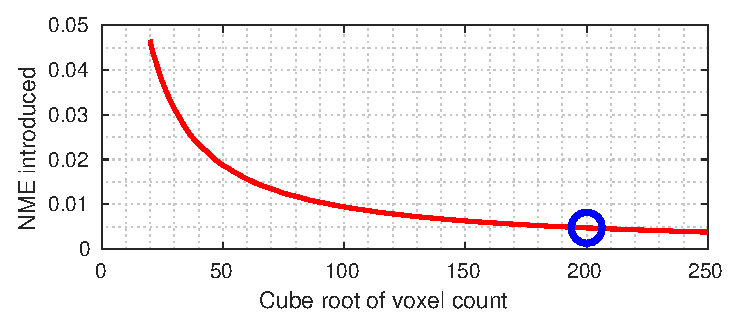
\includegraphics[width=0.9\linewidth]{curves/voxerror.eps}
  \caption[Error due to voxelisation]{The error introduced due to
    voxelisation, shown as a function of volume density.}
  \label{fig:voxerror}
\end{figure}

\subsection{Volumetric Regression Networks}


In this section, we describe the proposed volumetric regression
network, exploring several architectural variations described in
detail in the following subsections:

\textbf{Volumetric Regression Network (VRN)}. We wish to learn a
mapping from the 2D facial image to its corresponding 3D volume
$f: \mathbf{I} \rightarrow \mathbf{V}$. Given the training set of 2D
images and constructed volumes, we learn this mapping using a CNN. Our
CNN architecture for 3D segmentation is based on the ``hourglass
network'' of \cite{newell2016stacked} an extension of the fully
convolutional network of \cite{long2015fully} using skip connections
and residual learning \cite{he2015deep}. Our volumetric architecture
consists of two hourglass modules which are stacked together without
intermediate supervision. The input is an RGB image and the output is
a volume of $192\times 192\times 200$ of real values. This
architecture is shown in Figure~\ref{fig:cnnbaseline}. As it can be
observed, the network has an encoding/decoding structure where a set
of convolutional layers are firstly used to compute a feature
representation of fixed dimension. This representation is further
processed back to the spatial domain, re-establishing spatial
correspondence between the input image and the output volume. Features
are hierarchically combined from different resolutions to make
per-pixel predictions. The second hourglass is used to refine this
output, and has an identical structure to that of the first one.

\begin{figure*}
  \centering
  \begin{subfigure}[t]{1\textwidth}
    \centering
    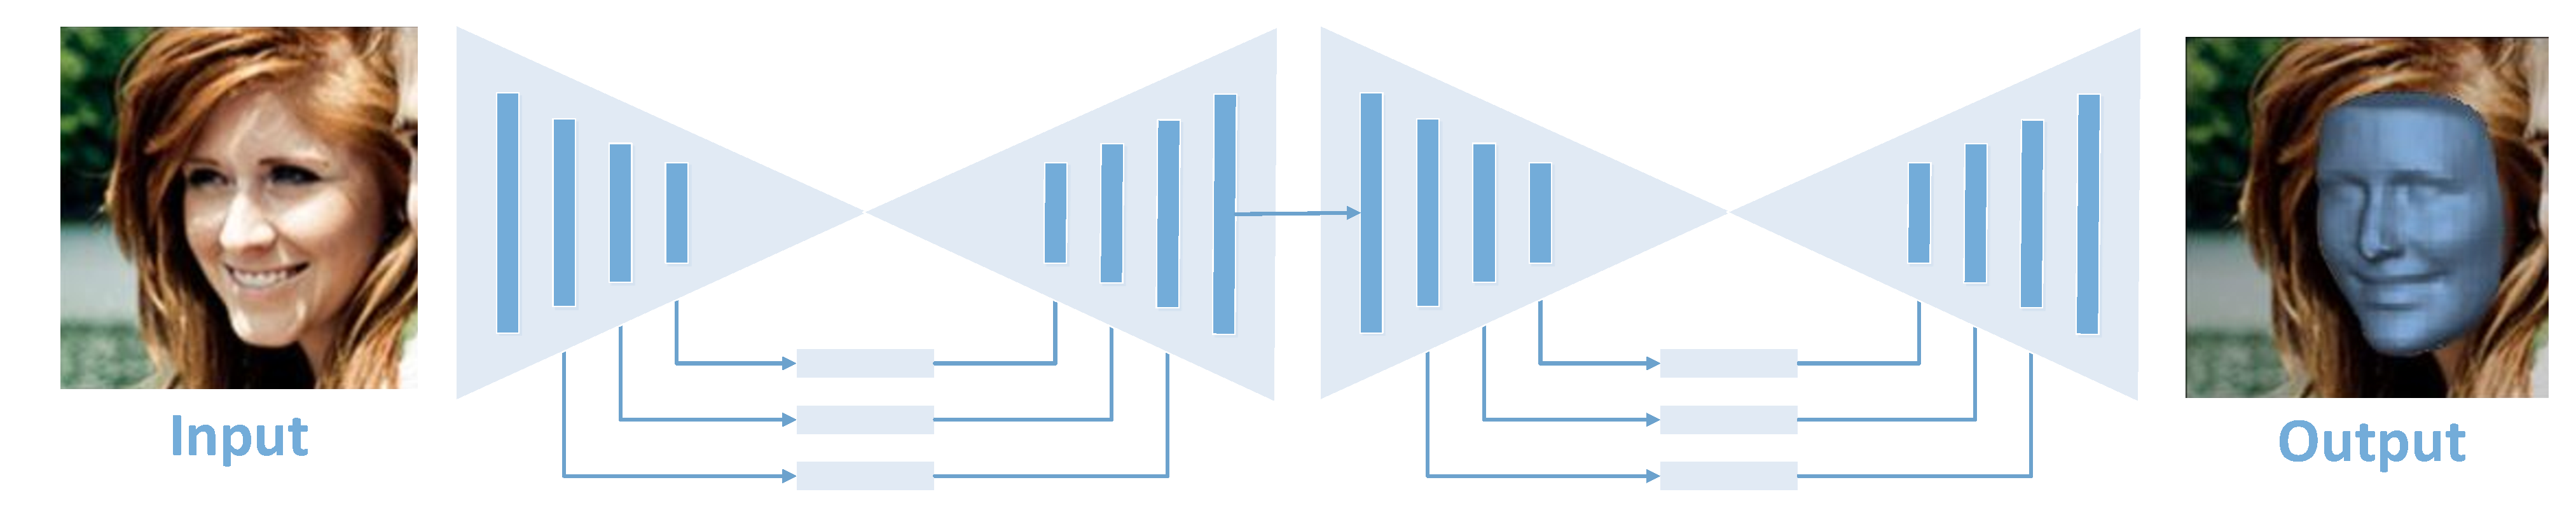
\includegraphics[width=0.81\linewidth]{img/baseline.pdf}
    \caption[Baseline reconstruction architecture]{The proposed
      \textit{Volumetric Regression Network (VRN)} accepts as input an
      RGB input and directly regresses a 3D volume completely bypassing
      the fitting of a 3DMM. Each rectangle is a residual module of 256
      features.}

    \label{fig:cnnbaseline}
  \end{subfigure}
  ~
  \begin{subfigure}[t]{1\textwidth}
    \centering
    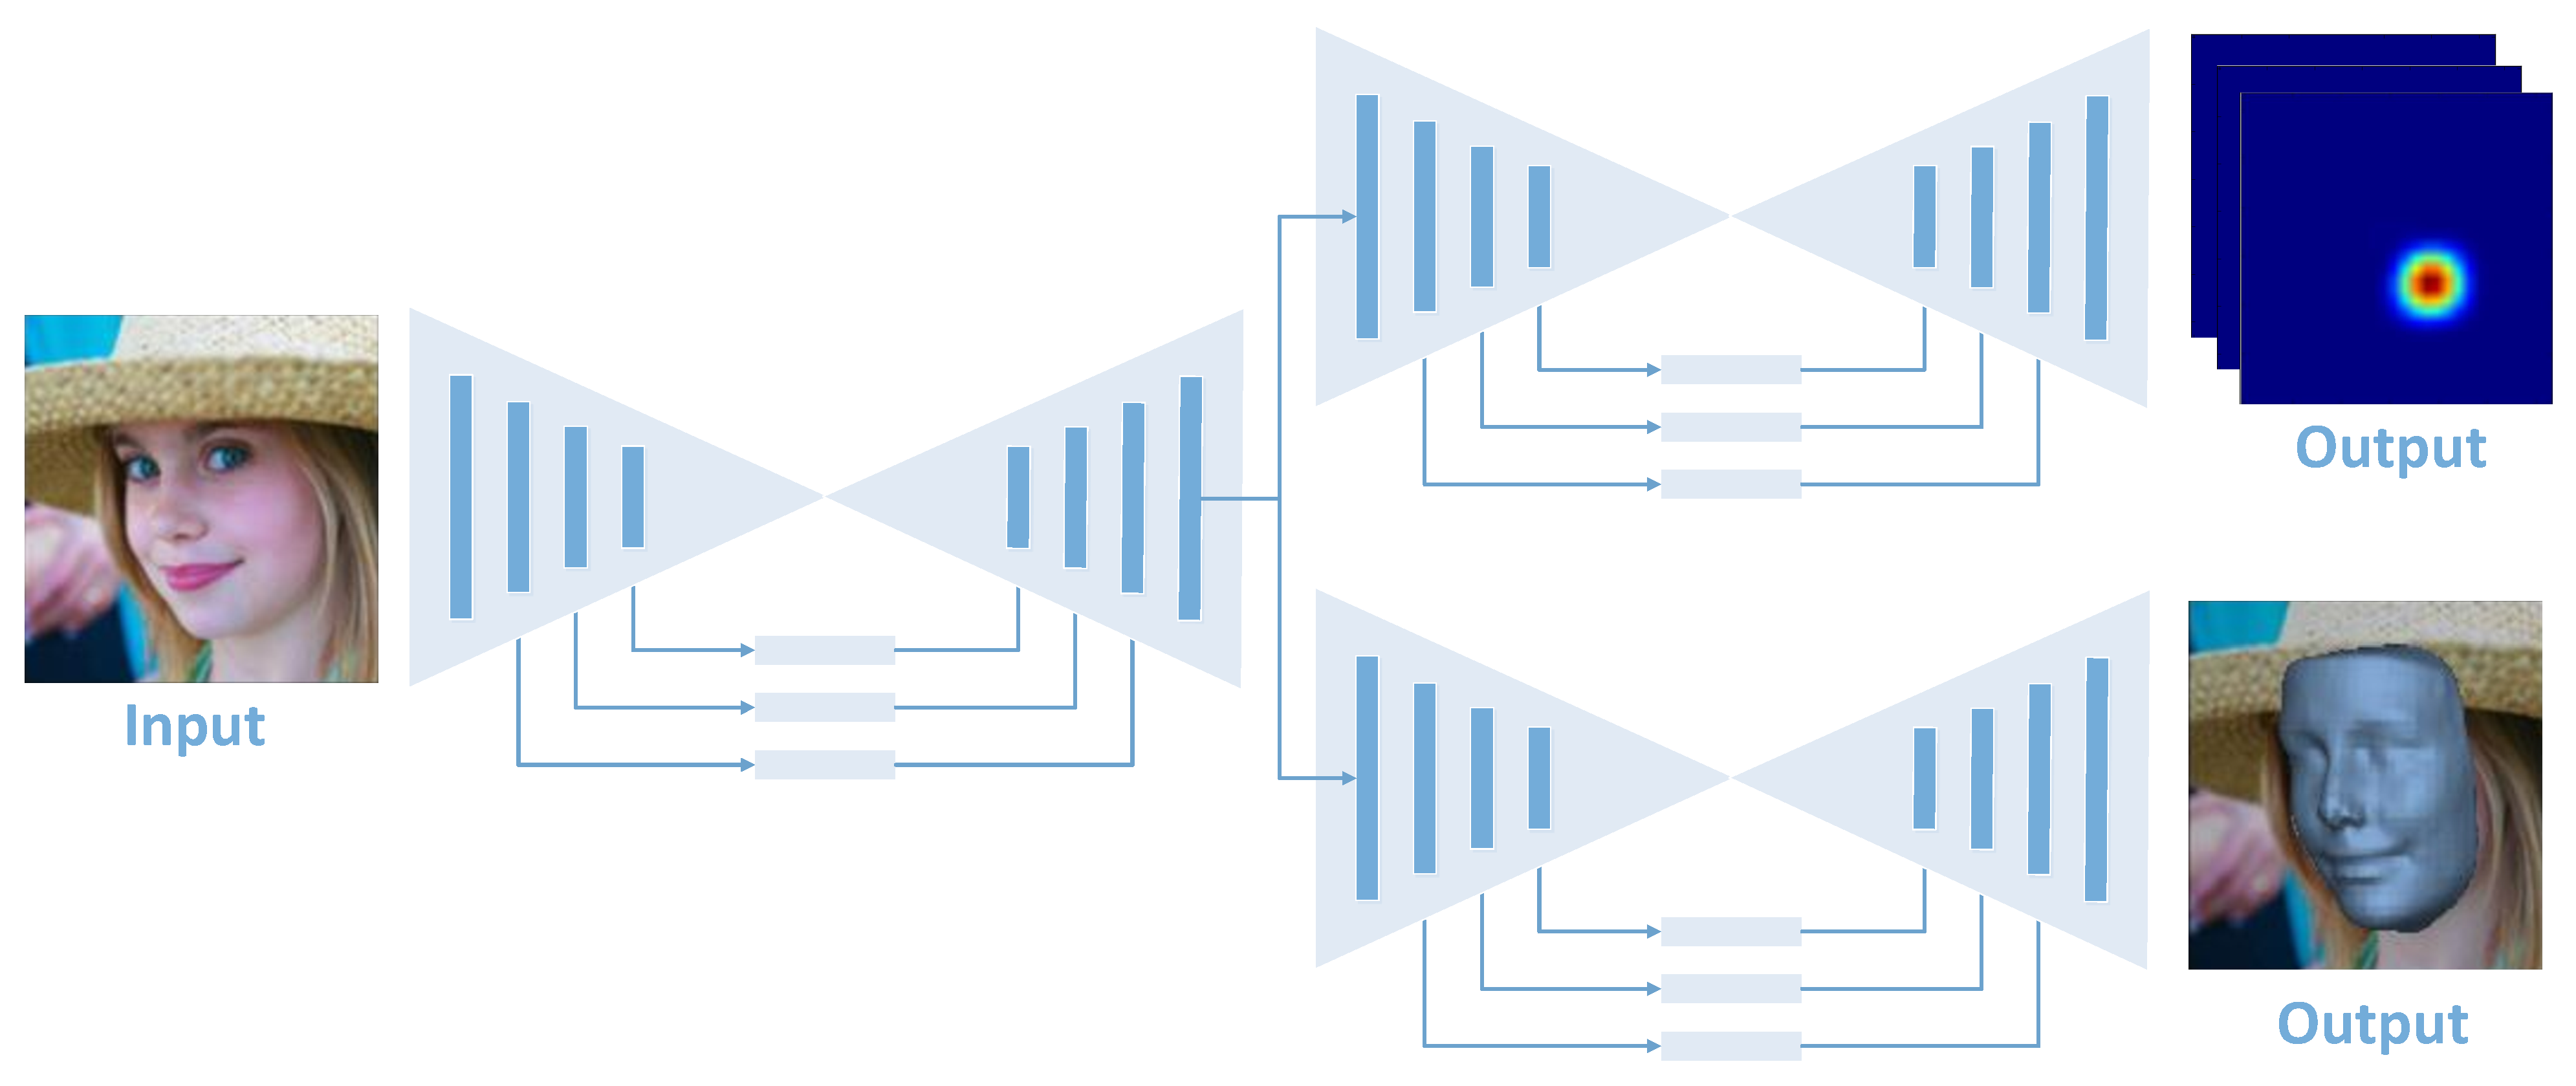
\includegraphics[width=0.6\linewidth]{img/multitask.pdf}
    \caption[Multitask reconstruction architecture]{The proposed
      \textit{VRN - Multitask} architecture regresses both the 3D facial
      volume and a set of sparse facial landmarks.}
    \label{fig:cnnmultitask}
    \vspace{-2mm}
  \end{subfigure}
  ~
  \begin{subfigure}[t]{0.98\textwidth}
    \centering
    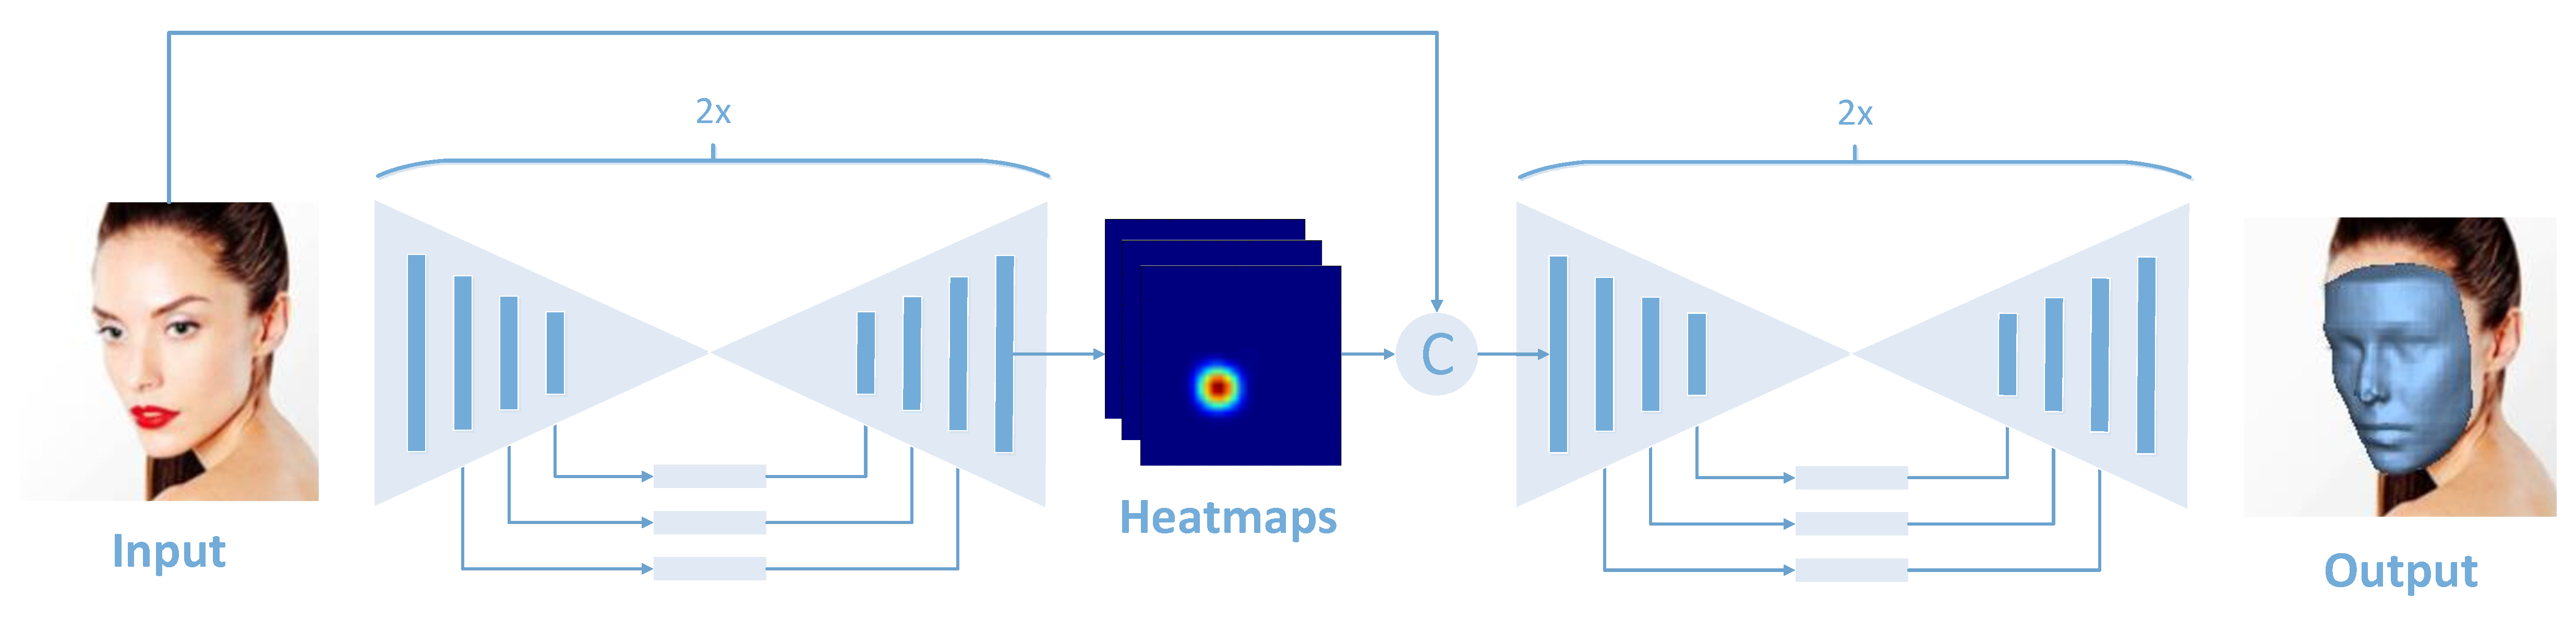
\includegraphics[width=\linewidth]{img/guided.pdf}
    \caption[Guided reconstruction architecture]{The proposed
      \textit{VRN - Guided} architecture firsts detects the 2D
      projection of the 3D landmarks, and stacks these with the original
      image. This stack is fed into the reconstruction network, which
      directly regresses the volume.}
    \label{fig:guidednet}
  \end{subfigure}
  ~
  \caption[Overview of proposed architectures]{An overview of the
    proposed three architectures for Volumetric Regression:
    \textit{Volumetric Regression Network (VRN)}, \textit{VRN -
      Multitask} and \textit{VRN - Guided}.}
  \label{fig:cnnall}
  \vspace{-5mm}
\end{figure*}

We train our volumetric regression network using the sigmoid cross
entropy loss function:
\begin{equation} l_{1} = \sum\limits_{w=1}^{W}
  \sum\limits_{h=1}^{H}\sum\limits_{d=1}^{D}[V_{whd}\log
  \widehat{V}_{whd}+(1-V_{whd})\log(1-\widehat{V}_{whd})],
\end{equation} where $\widehat{V}_{whd}$ is the corresponding Sigmoid
output at voxel $\{w,h,d\}$ of the regressed volume. In the case of
\textit{VRN - Multitask}, the same loss is applied to both tails of
the network with even weightings. Similarly, in \textit{VRN - Guided},
the loss is also applied to the heatmap regression and hence the loss
is summed during backpropagation.

Each residual module of all three of our architectures consists of 256
feature spatial convolutions.

At test time, and given an input 2D image, the network regresses a 3D
volume from which the outer 3D facial mesh is recovered. Rather than
making hard (binary) predictions at pixel level, we found that the
soft sigmoid output is more useful for further processing. Both
representations are shown in Figure~\ref{fig:roughvssmooth} where
clearly the latter results in smoother results. Finally, from the 3D
volume, a mesh can be formed by generating the iso-surface of the
volume. If needed, correspondence between this variable length mesh
and a fixed mesh can be found using Iterative Closest Point (ICP).

\textbf{VRN - Multitask}. We also propose a Multitask VRN, shown in
Figure~\ref{fig:cnnmultitask}, consisting of three hourglass
modules. The first hourglass provides features to a fork of two
hourglasses. The first of this fork regresses the 68 iBUG landmarks
\cite{sagonas2013semi} as 2D Gaussians, each on a separate
channel. The second hourglass of this fork directly regresses the 3D
structure of the face as a volume, as in the aforementioned unguided
volumetric regression method. The goal of this multitask network is to
learn more reliable features which are better suited to the two tasks.


\begin{figure}
  \centering
  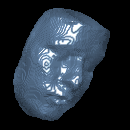
\includegraphics[width=0.2\linewidth]{img/example_rough.png}
  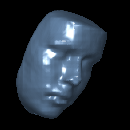
\includegraphics[width=0.2\linewidth]{img/example_smooth.png}
  \caption[Binary vs Real volumes]{Comparison between making hard
    (binary) vs soft (real) predictions. The latter produces a
    smoother result.}
  \label{fig:roughvssmooth}
  \vspace{-4mm}
\end{figure}


\textbf{VRN - Guided}. We argue that reconstruction should benefit
from firstly performing a simpler face analysis task; in particular we
propose an architecture for volumetric regression guided by facial
landmarks. To this end, we train a stacked hourglass network which
accepts guidance from landmarks during training and inference. This
network has a similar architecture to the unguided volumetric
regression method, however the input to this architecture is an RGB
image stacked with 68 channels, each containing a Gaussian ($\sigma =
1$, approximate diameter of 6 pixels) centred on each of the 68
landmarks. This stacked representation and architecture is
demonstrated in Figure~\ref{fig:guidednet}. During training we used the
ground truth landmarks while during testing we used a stacked
hourglass network trained for facial landmark localisation. We call
this network \textit{VRN - Guided}.




\subsection{Training}

% Trained with RMSProp
Each of our architectures was trained end-to-end using RMSProp with an
initial learning rate of $10^{-4}$, which was lowered after 40 epochs
to $10^{-5}$. This training protocol remained fixed for all
architectures to avoid bias. The number of epochs were chosen based on
the rate at which the learning rate fell during training of
\textit{VRN} and some tests using the testing set of the
HELEN~\cite{le2012interactive} images from
300W~\cite{sagonas2013semi} as validation. During training,
random augmentation was applied to each input sample (face image) and
its corresponding target (3D volume): we applied in-plane rotation
$r\in[-45^{\circ}, ..., 45^{\circ}]$, translation
$t_z,t_y\in[-15,...,15]$ and scale $s\in [0.85,...,1.15]$ jitter. In
20\% of cases, the input and target were flipped
horizontally. Finally, the input samples were adjusted with some
colour scaling on each RGB channel selected uniformly
$c_r,c_g,c_b \in \{0.6,...,1.4\}$.

In the case of the \textit{VRN - Guided}, the landmark detection
module was trained to regress Gaussians with standard deviation of
approximately 3 pixels ($\sigma = 1$). We noticed near negligible
reduction in 3D reconstruction performance when training with
different standard deviations.

% dataset selection

% Gaussian size (sigma 1)
% Learning rate

\section{Results} \label{S:Results}

\subsection{Evaluation Datasets}

We used three different datasets for quantifying the performance of
our method. The dataset AFLW2000-3D allows for unbiased and fair
comparison with other methods. The remaining two, BU-4DFE and
Florence, have to be rendered, but allows us to quantify performance
across pose and expression with greater accuracy. These three datasets
are discussed in more detail below.

\paragraph{(a) AFLW2000-3D} As our target was to test
our network on totally unconstrained images, we firstly conducted
experiments on the AFLW2000-3D~\cite{zhu2016face} dataset which
contains 3D facial meshes for the first 2000 images from AFLW
\cite{aflw2011}.

\paragraph{(b) BU-4DFE} We also conducted experiments on rendered
images from BU-4DFE~\cite{yin2008high}. We rendered each participant
for both Happy and Surprised expressions with three different pitch
rotations between $-20$ and $20$ degrees. For each pitch, seven roll
rotations from $-80$ to $80$ degrees were also rendered. Large
variations in lighting direction and colour were added randomly to
make the images more challenging. We show some example renderings in
the first row (a) of Figure~\ref{fig:example_renderings}.

\paragraph{(c) Florence}
Finally, we conducted experiments on rendered images from the
Florence~\cite{masi2d3dFaceData} dataset. Facial images were rendered
in a similar fashion to the ones of BU-4DFE but for slightly different
parameters: Each face is rendered in 20 difference poses, using a
pitch of -15, 20 or 25 degrees and each of the five evenly spaced
rotations between -80 and 80. We show some example renderings in the
second (b) row of Figure~\ref{fig:example_renderings}.

\begin{figure}
  \centering
  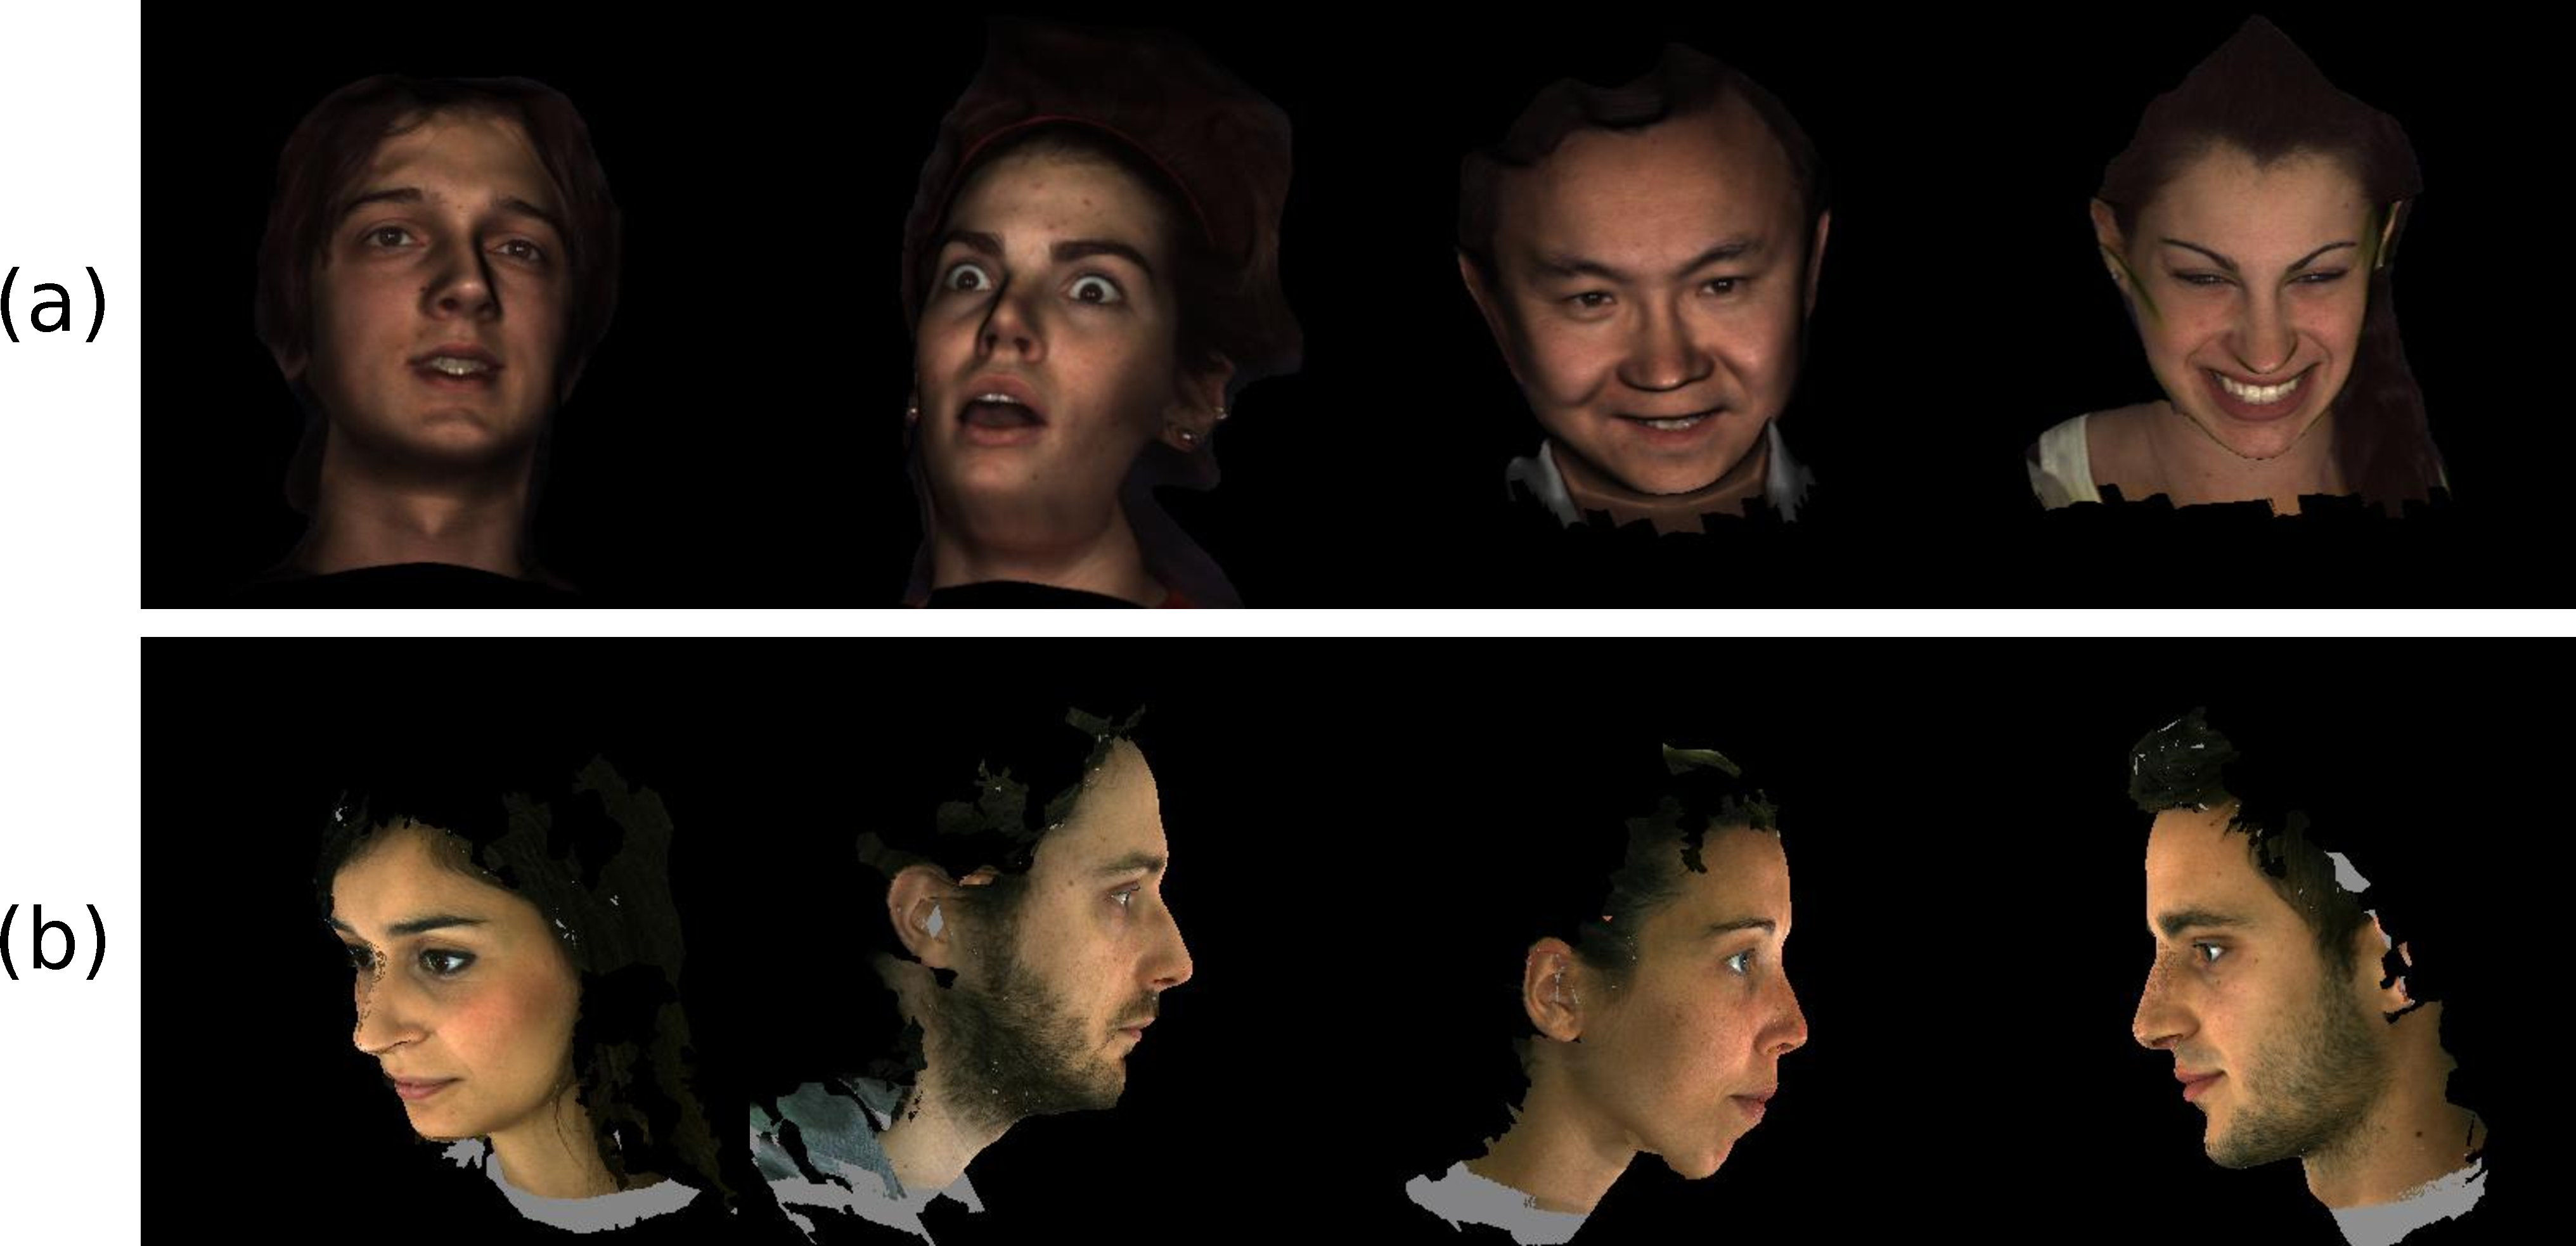
\includegraphics[width=0.9\linewidth]{img/rendering_examples.pdf}
  \caption[Example BU-4DFE and Florence renderings]{Example renderings
    from the BU-4DFE \textbf{(a)} and Florence \textbf{(b)}.}
  \label{fig:example_renderings}
\end{figure}

\subsection{Evaluation metric} To measure the accuracy of reconstruction for
each face, we used the Normalised Mean Error (NME) defined as the
average per vertex Euclidean distance between the estimated and ground
truth reconstruction normalised by the outer 3D interocular distance:

\begin{equation}
  \textrm{NME} = \frac{1}{N} \sum_{k=1}^{N} \frac{||\mathbf{x}_k-\mathbf{y}_{k} ||_{2} }{d}, \label{eq:err}
\end{equation}
\label{eq:3d_nme}
where $N$ is the number of vertices per facial mesh, $d$ is the 3D
outer interocular distance and $\mathbf{x}_k$,$\mathbf{y}_k$ are
vertices of the grouthtruth and predicted meshes. This outer
interocular distance is the distance between the two lateral canthus,
which is the most outer part of the eye. As this is in 3D, the
distance remains fixed even when the face is rotated. The error is
calculated on the face region only on approximately 19,000 vertices
per facial mesh. Notice that when there is no point correspondence
between the ground truth and the estimated mesh, ICP was used but only
to establish the correspondence, i.e. the rigid alignment was not
used. If the rigid alignment is used, we found that, for all methods,
the error decreases but it turns out that the relative difference in
performance remains the same. For completeness, we included these
results in Section~\ref{sec:faceicpres}.


\subsection{Evaluation}

We performed cross-database experiments only, on 3 different
databases, namely AFLW2000-3D, BU-4DFE, and Florence reporting the
performance of all the proposed networks (\textit{VRN}, \textit{VRN -
  Multitask} and \textit{VRN - Guided}) along with the performance of
two state-of-the-art methods, namely 3DDFA \cite{zhu2016face} and EOS
\cite{huber2016multiresolution}. Both methods perform 3DMM
fitting (3DDFA uses a CNN), a process completely bypassed by \textit{VRN}.


% Don't really think this figure demonstrates what we want it to.
% \begin{figure}
%   \centering
%   \begin{tabular}{m{3cm}m{11cm}}
%     Image        & 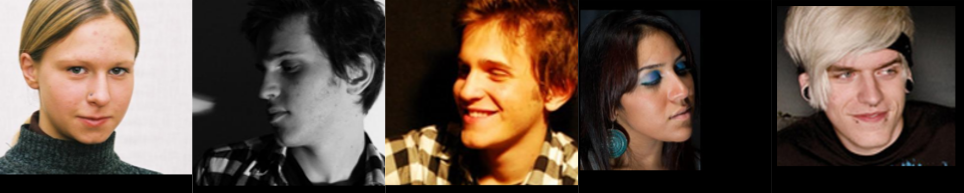
\includegraphics[width=11cm]{img/comparison_r1.png} \\
%     VRN          & 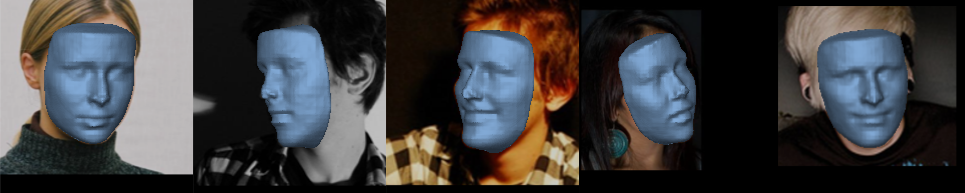
\includegraphics[width=11cm]{img/comparison_r3.png} \\
%     VRN - Guided & 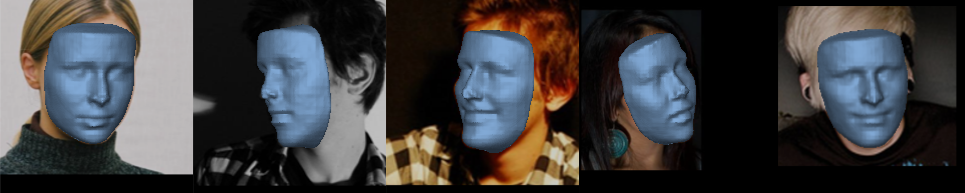
\includegraphics[width=11cm]{img/comparison_r3.png} \\
%   \end{tabular}
% \end{figure}

Our results can be found in Table~\ref{tab:overview} and
Figures~\ref{roc:aflw2000},~\ref{roc:bu4dfe} and~\ref{roc:florence}.
Visual results of the proposed \textit{VRN - Guided} on some very
challenging images from AFLW2000-3D can be seen in
Figure~\ref{fig:aflw2000res}. We show some failure cases in
Figure~\ref{fig:facefailure} where the images are very different to
what has been seen during training time. Finally, we show some example
results from some frames in the 300-VW~\cite{sagonas2013300} video
dataset in Figure~\ref{fig:face300vw}. From all of these results, we
can conclude the following:
\begin{enumerate}
\item Volumetric Regression Networks largely outperform 3DDFA and EOS
  on all datasets used for evaluation, statistically significant in
  all cases ($p < 0.01$, paired $t$-test). This verifies that directly
  regressing the 3D facial structure using the volumetric
  representation, is a much easier problem for CNN learning.
\item All VRNs perform well across the whole spectrum of facial poses,
  expressions and occlusions. Also, there are no significant performance
  discrepancies across different datasets (ALFW2000-3D seems to be
  slightly more difficult).
\item The best performing VRN is the one guided by detected landmarks
  (\textit{VRN - Guided}), however at the cost of higher computational
  complexity: \textit{VRN - Guided} uses another stacked hourglass
  network for landmark localization.
\item \textit{VRN - Multitask} does not always perform better than the
  plain VRN (in fact on BU-4DFE it performs worse), not justifying the
  increase of network complexity. The results are not significant on
  any dataset ($p > 0.10$, paired $t$-test).  It seems that it might
  be preferable to train a network to focus on the task in hand.
\end{enumerate}

\noindent Details about our experiments are given in the proceeding subsections.



\begin{figure}
  \centering
  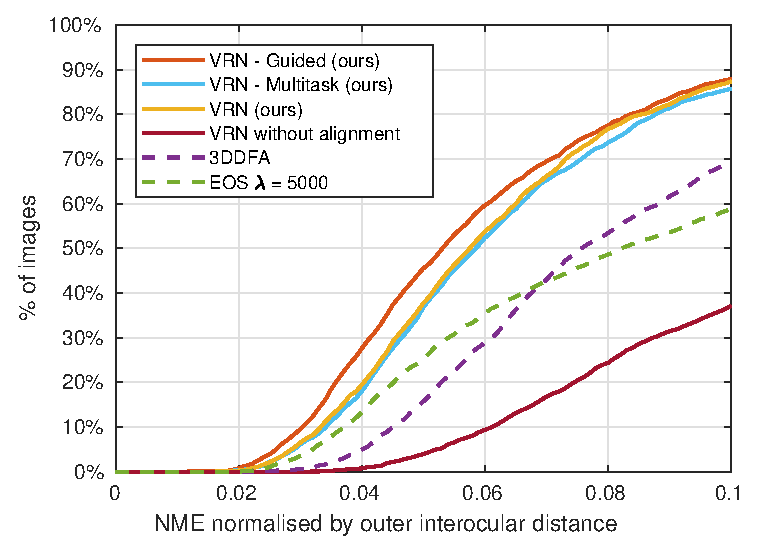
\includegraphics[width=0.75\linewidth]{curves/aflw.eps}
  \caption[NME performance on AFLW2000-3D images]{NME-based
    (Equation~\ref{eq:3d_nme}) performance on in-the-wild ALFW2000-3D
    dataset. The proposed \textit{Volumetric Regression Networks}, and
    EOS and 3DDFA are compared. Please note that ``VRN - without
    allignment'' refers to a VRN where a frontal face is always
    regressed, regardless of input pose, discussed in
    Section~\ref{sec:spatialimportance}.}
  \label{roc:aflw2000}
\end{figure}

\begin{figure}
  \centering
  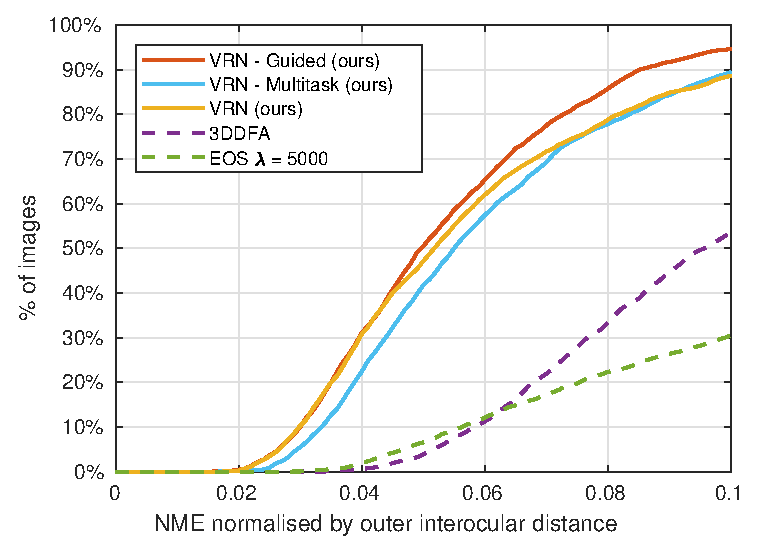
\includegraphics[width=0.75\linewidth]{curves/bu4dfe.eps}
  \caption[NME performance on BU-4DFE renderings]{NME-based
    (Equation~\ref{eq:3d_nme}) performance on renderings from
    BU-4DFE. The proposed \textit{Volumetric Regression Networks}, and
    EOS and 3DDFA are compared.}
  \label{roc:bu4dfe}
\end{figure}

\begin{figure}
  \centering
  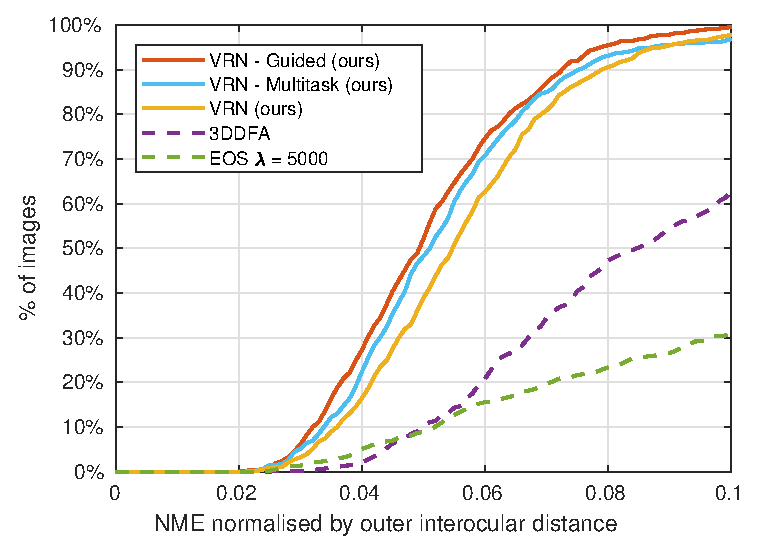
\includegraphics[width=0.75\linewidth]{curves/florence.eps}
  \caption[NME performance on Florence renderings]{NME-based
    (Equation~\ref{eq:3d_nme}) performance on our large pose
    renderings of the Florence dataset. The proposed
    \textit{Volumetric Regression Networks}, and EOS and 3DDFA are
    compared.}
  \label{roc:florence}
\end{figure}




\begin{figure}
  \centering
  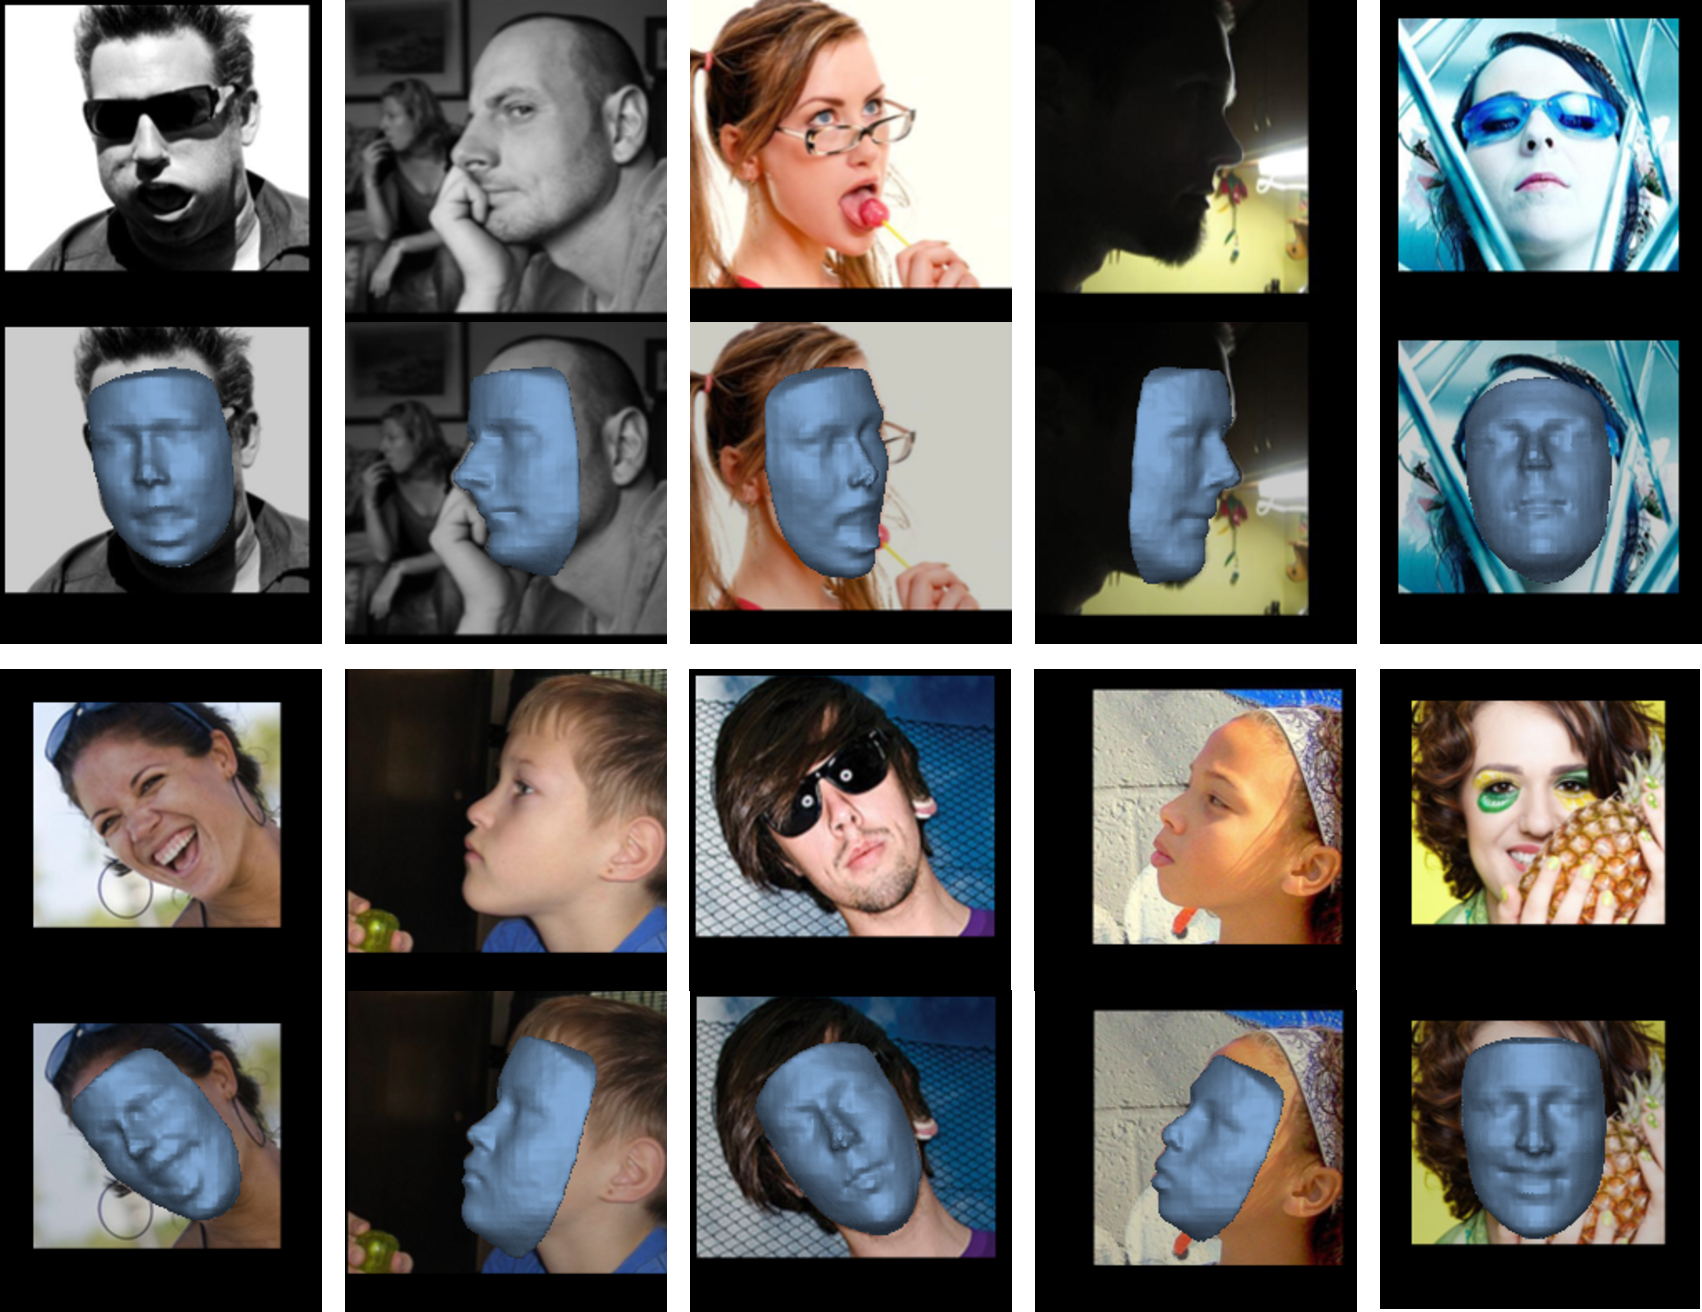
\includegraphics[width=0.7\linewidth]{img/aflw2000res.pdf}
  \caption[Visual results on AFLW2000-3D dataset]{Some visual results
    from the AFLW2000-3D dataset generated using our \textit{VRN -
      Guided} method.}
  \label{fig:aflw2000res}
  \vspace{-4mm}
\end{figure}


\begin{figure}
  \centering
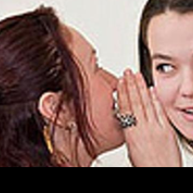
\includegraphics[width=3.4cm]{img/failures/image00400_img.png}
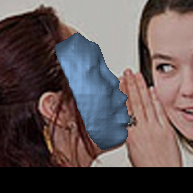
\includegraphics[width=3.4cm]{img/failures/image00400_vol.png} \hspace{2mm}
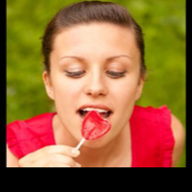
\includegraphics[width=3.4cm]{img/failures/image00782_img.png}
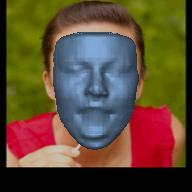
\includegraphics[width=3.4cm]{img/failures/image00782_vol.png}  \\ [0.5mm]

\includegraphics[width=3.4cm]{img/failures/image00795_img.png}
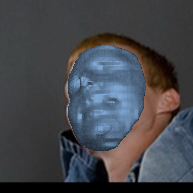
\includegraphics[width=3.4cm]{img/failures/image00795_vol.png} \hspace{2mm}
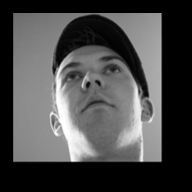
\includegraphics[width=3.4cm]{img/failures/image01038_img.png}
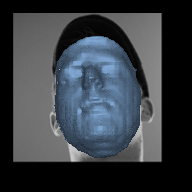
\includegraphics[width=3.4cm]{img/failures/image01038_vol.png}  \\ [0.5mm]
\includegraphics[width=3.4cm]{img/failures/image01624_img.png}
\includegraphics[width=3.4cm]{img/failures/image01624_vol.png} \hspace{2mm}
\includegraphics[width=3.4cm]{img/failures/image02026_img.png}
\includegraphics[width=3.4cm]{img/failures/image02026_vol.png}
\caption[Some very difficult failure cases]{Some failure cases on
  AFLW2000 from our \textit{VRN - Guided} network. In general, these
  images are poses which are not seen in the training set.}
\label{fig:facefailure}
\end{figure}

\begin{figure}
  \centering
  \includegraphics[width=0.9\linewidth]{img/300vw.png}
  \caption[Visual results on the 300VW dataset]{Some example results
    from frames of the 300VW dataset.}
  \label{fig:face300vw}
\end{figure}


\subsubsection{Comparison with state-of-the-art}
We compared against state-of-the-art 3D reconstruction methods for
which code is publicly available. These include the very recent
methods of 3DDFA~\cite{zhu2016face}, and
EOS~\cite{huber2016multiresolution}. For EOS we used a large
regularisation parameter $\lambda = 5000$ which we found to offer the
best performance for most images. The method uses 2D landmarks as
input, so for the sake of a fair comparison a stacked hourglass for 2D
landmark detection was trained for this purpose. Our tests were
performed using v0.12 of EOS.


\subsection{Results with ICP Alignment}
\label{sec:faceicpres}

We present results where ICP has been used not only to find the
correspondence between the groundtruth and predicted vertices, but
also to remove the rigid transformation between them. ICP was applied
after the surface extraction was used to create the mesh. We find that
this offers a marginal improvement to all methods. However, the
relative performance remains mostly the same between each
method. Results on AFLW2000~\cite{zhu2016face},
BU4DFE~\cite{yin2008high} and Florence~\cite{masi2d3dFaceData} can be
seen in Figs.~\ref{roc:aflw2000icp},~\ref{roc:bu4dfeicp}
and~\ref{roc:florenceicp} respectively. Numeric results can be found
in Table~\ref{tab:overviewicp}.

\begin{table}
  \caption[Numerical performance of 3D face reconstruction with
  ICP]{Reconstruction accuracy on AFLW2000-3D, BU4DFE and Florence in
    terms of NME (Equation~\ref{eq:3d_nme}) where ICP has been used to
    remove the rigid transformation. Lower is better. }
  \label{tab:overviewicp}
  \centering\vspace{1mm}
  \small
\begin{tabular}{|l||c|c|c|}
  \hline
  \textbf{Method}   & \textbf{AFLW2000} & \textbf{BU4DFE} & \textbf{Florence} \\
  \hline\hline
  VRN               & 0.0605 & 0.0514 & 0.0470   \\
  VRN - Multitask   &   0.0625    & 0.0533     & 0.0439        \\
  VRN - Guided      & \textbf{0.0543} & \textbf{0.0471} & \textbf{0.0429}   \\

\hline
  3DDFA~\cite{zhu2016face}             & 0.1012 & 0.1144 & 0.0784   \\
  EOS~\cite{huber2016multiresolution}  & 0.0890 & 0.1456 & 0.1200   \\
  \hline
\end{tabular}
\end{table}

\begin{figure}
  \centering
  \includegraphics[width=0.75\linewidth]{curves-icp/aflw.eps}
  \caption[NME performance on AFLW2000-3D with ICP
  Alignment]{NME-based (Equation~\ref{eq:3d_nme}) performance on the
    in-the-wild AFLW2000-3D dataset, where ICP has been used to remove
    the rigid transformation. The proposed \textit{Volumetric
      Regression Networks}, and EOS and 3DDFA are compared.}
  \label{roc:aflw2000icp}
\end{figure}

\begin{figure}
  \centering
  \includegraphics[width=0.75\linewidth]{curves-icp/bu4dfe.eps}
  \caption[NME performance on BU4DFE with ICP Alignment]{NME-based
    (Equation~\ref{eq:3d_nme}) performance on our large pose and
    expression renderings of the BU4DFE dataset, where ICP has been
    used to remove the rigid transformation. The proposed
    \textit{Volumetric Regression Networks}, and EOS and 3DDFA are
    compared.}
  \label{roc:bu4dfeicp}
\end{figure}

\begin{figure}
  \centering
  \includegraphics[width=0.75\linewidth]{curves-icp/florence.eps}
  \caption[NME performance on Florence with ICP Alignment]{NME-based
    (Equation~\ref{eq:3d_nme}) performance on our large pose
    renderings of the Florence dataset, where ICP has been used to
    remove the rigid transformation. The proposed \textit{Volumetric
      Regression Networks}, and EOS and 3DDFA are compared.}
  \label{roc:florenceicp}
\end{figure}


\section{Importance of spatial alignment}
\label{sec:spatialimportance}

Our approach to 3D face reconstruction preserves the spatial alignment
between input and output. That is to say that the regressed 3D
geometry should be capable of segmenting the input face from the
background, given a 2D orthographic projection of the volume. A 3D
reconstruction method is described in~\cite{choy20163d} which accepts
as input one or more images, and as output, produces a small 3D volume
of $32 \times 32 \times 32$ using an LSTM. In an attempt to explore
what the repercussions of ignoring spatial alignment are, we trained a
variant of \textit{VRN} which regresses a frontal version of the face,
i.e. a face of fixed orientation, regardless of input pose, as
in~\cite{choy20163d}. We call this fixed-pose variant of our method
\textit{VRN - without alignment}. We also attempted to train a network
using the code from~\cite{choy20163d} on downsampled versions of our
volumes. Unfortunately we were unable to get the network to learn
anything and found that the loss would now reduce.

Although \textit{VRN - without alignment} produces a reasonable face,
it captures only a diminished expression. The shape for all faces
appears to remain almost identical across all images. This is very
noticeable in Figure~\ref{fig:frontal_visual}. Numeric comparison is
shown in Figure~\ref{roc:aflw2000}, as \textit{VRN - without
  alignment}. We believe that this further confirms that
\textbf{spatial alignment is of paramount importance} when performing
3D reconstruction in this way.

\begin{figure}
  \centering
  \includegraphics[width=0.7\linewidth]{img/frontal.png}
  \caption[Visual results when spatial alignment is ignored]{Result from
    \textit{VRN without alignment} (second columns), and a frontalised
    output from \textit{VRN - Guided} (third columns).}
  \label{fig:frontal_visual}
\end{figure}

\section{Ablation studies}
\label{chapter:face:sec:ablation}

In this section, we report the results of experiments aiming to shed
further light into the performance of the proposed networks. For all
experiments reported, we used the best performing \textit{VRN -
  Guided}.

\subsection{Effect of pose}

To measure the influence of pose on the reconstruction error, we
measured the NME (Equation~\ref{eq:3d_nme}) for different amounts of
yaw using all of our Florence~\cite{masi2d3dFaceData}
renderings. These were rendered at $\{-80, -40, 0, 40, 80\}$ degrees
of yaw for each of $\{-5, 0, 5\}$ degrees of pitch, for all 50
subjects in Florence. As shown in Figure~\ref{fig:effect_pose}, the
performance of our method decreases as the pose increases. This is to
be expected, due to less of the face being visible which makes
evaluation for the invisible part difficult. We believe that our error
is still very low considering the magnitude of these poses.



\subsection{Effect of expression} Certain expressions are usually
considered harder to accurately reproduce in 3D face reconstruction.
To measure the effect of facial expressions on performance, we
rendered frontal images in difference expressions from BU-4DFE (since
Florence only exhibits a neutral expression) and measured the
performance for each expression. We show the six acted facial
expressions which are available in BU-4DFE in
Figure~\ref{fig:bu4dfe_expressions}. These expressions are available
for all participants, of which there are 102. This kind of extreme
acted facial expressions generally do not occur in the training set,
yet as shown in Figure~\ref{fig:effect_expression}, the performance
variation across different expressions is quite minor.

\begin{figure}
  \centering
  \includegraphics[width=0.6\linewidth]{curves/ablation_pose.eps}
  \caption[Effect of pose]{The effect of pose on reconstruction
    accuracy in terms of NME (Equation~\ref{eq:3d_nme}) on the
    Florence dataset. The \textit{VRN - Guided} network was used.}
  \label{fig:effect_pose}
\end{figure}

\begin{figure}
  \centering
  \includegraphics[width=0.8\linewidth]{img/bu4dfe_expressions.pdf}
  \caption[The six facial expressions available in the BU-4DFE
  dataset]{The six facial expressions available in the BU-4DFE
    dataset~\cite{yin2008high}, rendered for the same participant.}
  \label{fig:bu4dfe_expressions}
\end{figure}

\begin{figure}
  \centering
  \includegraphics[width=0.7\linewidth]{curves/ablation_expression.eps}
  \caption[Effect of facial expressions]{The effect of facial
    expression on reconstruction accuracy in terms of NME
    (Equation~\ref{eq:3d_nme}) on the BU-4DFE dataset. The \textit{VRN
      - Guided} network was used.}
  \label{fig:effect_expression}
\end{figure}

\subsection{Effect of Gaussian size for guidance} We trained a
\textit{VRN - Guided}, however, this time, the facial landmark
detector network of the \textit{VRN - Guided} regresses larger
Gaussians ($\sigma = 2$ as opposed to the normal $\sigma = 1$). The
performance of the 3D reconstruction dropped by a negligible amount,
suggesting that as long as the Gaussians are of a sensible size,
guidance will always help.

\section{Architectural Experiments}
\label{sec:arcexp}

In this section we explore several variations and modifications to the
\textit{VRN - Guided} method, which may improve or impede
performance. We provide an overview of experiments along with NME
(Equation~\ref{eq:3d_nme}) in Table~\ref{tab:arcexpoverview}.

\begin{table*}
  \caption[Overview of architectural experiments]{An overview of the
    architectural experiments conducted. \textbf{Feats} refers to the
    number of features per convolution layer. Similarly,
    \textbf{VFeats} refers to the number of volumetric features per
    volumetric convolution (in most cases this has no value as the
    majority of the networks used in our experiments are 2D
    only). \textbf{Mod} refers to the number of Residual modules used
    sequentially in any one place of the hourglass. \textbf{Stack}
    refers to the number of hourglass networks in a single stack. The
    right most column points to the relevant section of the
    chapter. We also show the mean Normalised Mean Error (NME,
    Equation\ref{eq:3d_nme}) for all images of the AFLW2000 dataset in
    column \textbf{nNME}.}
  \label{tab:arcexpoverview}
  \centering
  \small
  \begin{tabular}{|r|| c|c|c|c || c || c|l|}
    \hline
    \textbf{Name} & \textbf{Feats} & \textbf{VFeats} & \textbf{Mod} & \textbf{Stack} &  \textbf{Para} & \textbf{mNME} & \textbf{Sec.} \\
    \hline\hline
    VRN - Guided             & 256    & ---     & 4        & 2  & $2.5\times 10^7$    & 0.0637 &   \\
    \hline
    Intermediate Supervis.   & 256    & ---     & 4        & 2  & $2.5\times 10^7$    & 0.0630 & \ref{sec:arc_intersup}  \\
    \hline
    Hourglass                & 256    & ---     & 8        & 1  & $2.5\times 10^7$    & 0.0621 &   \\
    Three Hourglass          & 256    & ---     & 3        & 3  & $2.8\times 10^7$    & 0.0632 & \ref{sec:arc_secvsmod}  \\
    Four Hourglass           & 256    & ---     & 2        & 4  & $2.7\times 10^7$    & 0.0639 &   \\
    \hline
    Hourglass Heavy          & 384    & ---     & 8        & 1  & $5.3\times 10^7$    & 0.0627 &   \\
    Hourglass Light          & 128    & ---     & 8        & 1  & $6.3\times 10^6$    & 0.0633 & \ref{sec:arc_params}  \\
    Hourglass Lighter        & 64     & ---     & 8        & 1  & $1.8\times 10^6$    & 0.0661 &   \\
    \hline
    Volumetric VRN           & 128    & 32      & 2        & 2  & $7.7\times 10^5$    & 0.0697 & \ref{sec:arc_volumetric} \\
    \hline
  \end{tabular}
\end{table*}

\subsection{On intermediate supervision}
\label{sec:arc_intersup}

As described in the original stacked hourglass
paper~\cite{newell2016stacked}, intermediate supervision is typically
used providing significant boost in performance. However, it was not
implemented for the basic \textit{VRN} or \textit{VRN - Guided}
networks. As an attempt to boost performance, we have trained an
identical network to \textit{VRN - Guided}, except with a supervising
loss after the first hourglass network. A very minor performance
improvement can be observed, as shown in
Table~\ref{tab:arcexpoverview}. Additionally, the corresponding curve
can be seen in Figure~\ref{fig:additionalexp}. We conclude that
intermediate supervision is not necessary to achieve high performance
for our 3D reconstruction experiment.

%It is possible that in
%\cite{newell2016stacked}, higher performance were observed by using
%intermediate supervision, simply because there were many more
%hourglasses in a stack.


\subsection{On increasing the number of stacks vs the number of modules}
\label{sec:arc_secvsmod}

Given a fixed computational budget one has two options when
implementing a Volumetric Regression Network: to increase the number
of stacks while decreasing the number of modules or vice versa.  An
interesting question which has now been answered yet is whether it is
better to have more stacked hourglasses or more modules per
hourglass. In this section, we attempt to quantify any performance
variation, at least for the task of 3D face reconstruction using
volumetric regression while keeping the number of parameters
approximately the same.

We evaluate three additional networks, each with different number of
hourglasses and modules, such that the total number of parameters
remains very similar. These results are shown in detail in
Table~\ref{tab:arcexpoverview} as One, Three or Four Hourglass. The
first of these additional networks consists of only one hourglass
network and eight modules. Interestingly, this performs the best out
of the three, suggesting that for this particular problem, perhaps it
is more optimal to increase the number of modules over the number of
hourglasses. This may also be observed from a single hourglass
outperforming \textit{VRN - Guided}, which again, may be due to higher
performance gains from more modules over stacked hourglasses.However,
it can also be observed that the performance difference between all
networks is very minor, suggesting that for our experiment as long as
the number of parameters remains roughly fixed good performance can be
achieved independently of the exact configuration of the hourglass
network.
%Perhaps our performance bottleneck is not the network but the dataset
%from which we are learning, which may be the case if there exists any
%noise.


\subsection{On varying the network parameters}
\label{sec:arc_params}

Having investigated the importance of network configuration in the
previous section, in this section we keep the architecture fixed and
instead vary the number of network parameters to quantify the the
performance impact. Hence, in this section we explore the influence of
number of parameters, and whether the performance will continue to
increase with the number of parameters, or the same performance can be
achieved with fewer parameters. If performance saturation has
occurred, the dataset has likely become the limiting factor, likely
due to variance in the training set, suggesting that it may be
possible to achieve a similar level of performance with fewer
parameters.

We explore 3 variants of the VRN, corresponding to different number of
parameters, namely \textit{Heavy}, \textit{Light} and
\textit{Lighter}. Their exact number of parameters and performance is
shown in Table~\ref{tab:arcexpoverview}. It can be observed that the
performance difference between \textit{Heavy} and \textit{Light} are
very minor. However, \textit{Lighter} resulted in a significant drop
in performance. With this information we can hypothesise that the
optimal number of parameters is the one corresponding to the
\textit{Light} network. We show a visual comparison between these
three networks in Figure~\ref{fig:heavy-light-lighter}: the visual
performance of the \textit{Lighter} network is clearly worse - the
surface is not as smooth and the facial expression is not captured as
clearly as in both \textit{Heavy} and \textit{Light}.

\subsection{A Volumetric Implementation}
\label{sec:arc_volumetric}

One of the main contributions of this chapter is to show that good
performance for 3D face reconstruction can be achieved even when 2D
spatial convolutions are used.  However, one might wonder why we
decided to use 2D convolutions for a 3D (volumetric) regression
task. The short answer is that training a 3D CNN is difficult and
highly resource intensive. Firstly, the activations are much larger,
consuming more memory leaving less space for parameters. Secondly, the
complexity of volumetric convolution is much higher than that of
standard spatial convolution, hence the time required to train such a
network is far greater, despite the potential for fewer parameters.

For completeness, we have trained a fully volumetric version of VRN
where we attempt to match this time the complexity in theoretical
floating point operations (FLOPS) for a single forward pass (as
opposed to matching the number of parameters) with that of a standard
VRN. We use theoretical FLOPS, as opposed to actual or raw number of
FLOPS, as frameworks such as CuDNN make numerous optimisations, which
often result in fewer operations. Unfortunately, this resulted in
having only 32 features per volumetric convolution.

Despite containing far fewer parameters than the standard VRN, the
training took over 10 days on two Titan X GPUs and had to be performed
with a batch size of 2. This is significantly slower than training the
standard VRN, which takes approximately 2 days on the same
hardware. We show the NME (Equation~\ref{eq:3d_nme}) for this network in
Table~\ref{tab:arcexpoverview}, along with a curve in
Figure~\ref{fig:additionalexp}. Unsurprisingly, the performance of
this method is quite poor, further illustrating the difficulty in
training 3D CNNs despite the problem being a volumetric one.

\subsection{Architectural Conclusions}
As we have seen from the past few experiments, performance in general
remains very similar despite architectural changes. Only after
reducing the number of parameters significantly were we able observe
any significant change. We conclude that with the guidance from
detected landmarks only, we are almost able to attain the best performance on
these datasets.

\begin{figure}
  \centering
  \includegraphics[width=0.75\linewidth]{curves2/aflw.eps}
  \caption[NME performance from architectural experiments]{Results in
    NME (Equation~\ref{eq:3d_nme}) from architectural experiments
    described in Section~\ref{sec:arcexp} on the AFLW2000 dataset,
    showing that in the majority of cases the performance is almost
    the same.}
  \label{fig:additionalexp}
\end{figure}

\begin{figure}
  \centering
  \includegraphics[width=0.75\linewidth]{img/heavy-light-lighter.png}
  \caption[Visual comparison of number of parameters]{A visual
    comparison between the \textit{Heavy}, \textit{Light} and
    \textit{Lighter} methods described in Section~\ref{sec:arc_params}
    on three images from the AFLW2000 dataset.}
  \label{fig:heavy-light-lighter}
\end{figure}



\section{Conclusions}

We proposed a direct approach to 3D facial reconstruction from a
single 2D image using volumetric CNN regression. To this end, we
proposed and exhaustively evaluated three different networks for
volumetric regression, reporting results that show that the proposed
networks perform well for the whole spectrum of facial pose, and can
deal with facial expressions as well as occlusions. We also compared
the performance of our networks against that of recent
state-of-the-art methods based on 3DMM fitting reporting large
performance improvement on three different datasets.  Future work may
include improving detail and establishing a fixed correspondence from
the isosurface of the mesh.


%%% Local Variables:
%%% TeX-master: "../thesis"
%%% End: % VRN for Faces
\graphicspath{{chapter_humans/}}
\chapter{3D Human Body Reconstruction from a Single Image via
  Volumetric Regression}
\label{chapter:human}

% \begin{abstract}
%   This paper proposes the use of an end-to-end Convolutional Neural
%   Network for direct reconstruction of the 3D geometry of humans via
%   volumetric regression. The proposed method does not require the
%   fitting of a shape model and can be trained to work from a variety
%   of input types, whether it be landmarks, images or segmentation
%   masks. Additionally, non-visible parts, either self-occluded or
%   otherwise, are still reconstructed, which is not the case with depth
%   map regression. We present results that show that our method can
%   handle both pose variation and detailed reconstruction given
%   appropriate datasets for training.

% \keywords{3D Reconstruction, Human Body Reconstruction, Volumetric
%   Regression, VRN, Single Image Reconstruction}
% \end{abstract}

\begin{figure}[h!]
  \centering
  \includegraphics[width=0.8\linewidth]{img/demo.png}
  \caption[Example reconstructions]{Some example results using our
    method when trained with a high quality detailed training set.}
  \label{fig:topdemo}
\end{figure}


\section{Introduction}


3D reconstruction is the process of estimating the 3D geometry from
one or more 2D images. In this work, we focus on reconstruction of the
human body from a single image, including the non-visible parts which
have been self-occluded. Our method builds upon that
of~\cite{jackson2017vrn} where a 3D face is directly regressed from a
single image, using what they refer to as a ``Volumetric Regression
Network'' (VRN). In this paper, we show that the same idea can be applied to
other deformable objects, in particular, the human body. This poses an
array of challenges which are not present when reconstructing the
face. While we are still only reconstructing an object of a single
class, the body has many more axes of rotation compared to a face. As
such, human body reconstruction is often considered to be a very
difficult problem.

\paragraph{Motivation.} The pipelines required for 3D human
reconstruction (and 3D reconstruction in general) are typically based
on solving difficult non-convex optimisation problems. Perhaps the
most common approach to 3D human body reconstruction is to fit a shape
model. For example, the recent method of \cite{bogo2016smplify}, uses
optimisation to fit a 3D shape model to 2D body joints. However,
optimisation methods are sensitive to initialization and are easily
trapped to local minima, both of which are exacerbated by occlusions
and potential scale changes.

In this work, we aim to significantly reduce the complexity of
standard 3D human reconstruction techniques - to the point where it
could just as easily be treated as a segmentation task. We do this by
directly regressing a volumetric representation of the 3D geometry
using a standard, spatial, CNN architecture, where the regressed
volumetric structure is spatially aligned with the input. Notably, we
do \textbf{not} regress a depth map; the 3D structure is regressed as
slices and recovered from its volumetric representation using a
standard surface extraction algorithm, such as Marching
Cubes~\cite{lorensen1987marching}. In summary, our main contributions
in this work are as follows:

\begin{enumerate}

\item We are the first to apply volumetric regression
  networks~\cite{jackson2017vrn} to the problem to human body
  reconstruction, not just human faces.

\item We propose several improvements to the network architecture
  described in~\cite{jackson2017vrn}, which show significant
  performance improvements. These include introducing intermediate
  supervision, using more advanced residual modules and altering the network
  structure by increasing the number of hourglass modules by reducing
  the number of residual modules.

\item We show that VRN is capable of reconstructing complex poses when
  trained on a suitable dataset.

\item Finally, we show that given high quality training data, our
  method can learn to produce previously unseen, highly detailed, full
  3D reconstructions from only a single image. To the best of our
  knowledge, there is no other method capable of obtaining results
  with such high fidelity and reliability as ours.
\end{enumerate}

The remainder of the paper is structured as follows: First, a review
of closely related work on 3D human body reconstruction and human pose
estimation is given. We then describe our method, including the
volumetric representation we have already mentioned briefly, followed
by the datasets and the training procedure. Next we will discuss
several architectural variants of VRN, followed by results from a
network trained with pose-variant data, but little detail. Finally, we
will show results which have been generated by training a model with
highly detailed data.

% 3DMM fitting
% Depth estimation



% In~\cite{5597194} no fitting is performed. Instead, the closest
% pose from a dataset of many pre-existing reconstructions

\section{Closely Related Work}


In this section we will give an overview of recent and popular
approaches to human pose estimation (often a prerequisite to human
reconstruction) and 3D reconstruction methods, both working from
images and from landmarks.

\paragraph{Human Pose Estimation.} All modern approaches to estimating
the human pose are based on methods employing CNNs. These methods
generally fall into one of two categories. The first is to directly
regress the coordinates of the joints using an L2 (or similar)
loss~\cite{li20143d,park20163d,tekin2016structured,tekin2016direct,zhou2016deep,chen2016synthesizing,ghezelghieh2016learning}.
In particular,~\cite{park20163d} estimate the 3D pose by combining the
2D predictions with image features. An autoencoder is employed
in~\cite{tekin2016structured} to constrain the pose to something
plausible. Similarly,~\cite{zhou2016deep} have the same goal but
achieve this by using a kinematic model. Synthetic data is used for
the full training procedure in~\cite{chen2016synthesizing}, to ensure
that the network is trained with accurate data. However,
in~\cite{ghezelghieh2016learning}, they only augment their existing
training set with synthetic data. The second approach to CNN based
human pose estimation is to regress a
heatmap~\cite{zhou2016sparseness,pavlakos2017coarse,mehta2017vnect,bulat2016human}. In~\cite{zhou2016sparseness}
they do this from video. In~\cite{pavlakos2017coarse} they regress a
3D heatmap, which is a similar idea to our own work. Another temporal
based approach is described in~\cite{mehta2017vnect}, where the 2D
landmarks are first refined also as a heatmap. A part based heatmap
regression approach is shown in~\cite{bulat2016human}.

In this work, we do not aim to estimate the human pose as a set of
coordinates. Instead, we aim to reconstruct the full 3D geometry of
the human, from just a single image. This includes any parts of the
body which are self occluded. However, in doing so, we optionally make
use of information from a human pose estimation step, which is
provided to the network as 16 channels, each with a Guassian centred
above the respective landmark.


\paragraph{Reconstruction from Image.} Many human reconstruction
methods estimate the geometry from one or more images. For
example,~\cite{balan2007detailed,grest2005human,guan2009estimating}
fit a model based on a single RGB or grey scale images. In particular,
\cite{grest2005human} fit a skeleton model to the image by estimating
the scale and pose of each body part
separately. In~\cite{guan2009estimating}, they fit a shape model
initialised by a user clicking on separate body parts, assisted by a
segmentation mask. Another shape model based approach is proposed
in~\cite{balan2007detailed}, using the SCRAPE
model~\cite{anguelov2005scape}, which is fitted with a stochastic
optimisation step. A general shape fitting method for reconstruction
is proposed in~\cite{chen2010inferring}, where two Gaussian models are
used - one for shape and one for pose, by solving non-linear
optimisation problems. The authors demonstrate this method on human
bodies and sharks. In~\cite{jiang20103d}, a single image and
corresponding landmarks are used to lookup a similar human pose using
a kd-tree, containing about 4 million examples. A method intended for
multi-instance model fitting from a single image is described
in~\cite{Zanfir_2018_CVPR}.

Several methods aim to estimate the 3D geometry using only the
landmarks extracted via human pose
estimation~\cite{bogo2016smplify,ramakrishna2012reconstructing}. Particularly,
SMPLify~\cite{bogo2016smplify} (which uses the SMPL
model~\cite{loper2015smpl}), was extended to also include further
guidance from an segmentation mask
in~\cite{varol2017learning}. However, such an approach will never be
able to capable of regressing finer details, unless information from
the image is also captured.

Aside from SCRAPE~\cite{anguelov2005scape} and
SMPL~\cite{loper2015smpl}, mentioned earlier, Dyna, the shape model
capable of capturing large variations in body shape is presented
in~\cite{Dyna:SIGGRAPH:2015}, but without an accompanying fitting
method from a single image. A very recent shape model called Total
Capture~\cite{Joo_2018_CVPR} captures many aspects of the body which
are typically ignored by other shape models, including the face and
hands.

Our work is different from all of the aforementioned methods in that
we do not regress parameters for a shape model, nor do we regress the
vertices directly. Further more, our method skips the model generation
step entirely, which avoids the need to find dense correspondence
between all training examples. Instead, we constrain the problem to
the spatial domain, and directly regress the 3D structure using
spatial convolutions in a CNN, via a volumetric representation from
which the full 3D geometry can be recovered.



\section{Method}

This section describes our proposed method, including the voxelisation
and alignment procedures.

\subsection{Volumetric Regression}

In this work, our goal is to reconstruct the full geometry of a human
body from just a single image.  There are several ways of estimating
the geometry using deep learning. The first is to directly regress the
vertices using a top-down network such as VGG~\cite{simonyan2014vgg}
or ResNet~\cite{he2015deep} trained with an L2 loss. This has at least
two disadvantages: firstly it requires the training data to be
resampled to have a fixed number of vertices, which implies finding
correspondence between all vertices of all meshes. Secondly, and more
importantly, training a network to directly regress a very large
number of vertices is hard. A common, and more efficient alternative
is to regress the parameters of a 3D shape model. However, as these
parameters are not scaled equally, it is necessary to employ
normalisation methods, such as weighting the outputs using the
Mahalanobis distance which has been also proven challenging to get it
working well~\cite{jackson2017vrn}. Additionally, 3D shape model based
approach are known to be good at capturing the coarse shape but less
able at capturing fine details (in the case of detailed 3D
reconstruction).

To eliminate the aforementioned learning challenges, we reformulate
the problem of 3D reconstruction by constraining it to the spatial
domain, using a standard convolutional neural network. Our approach
can be thought of as a type of image segmentation where the output is
a set of slices capturing the 3D geometry. Hence architecturally one
can use standard architectures for (say, semantic)
segmentation. Following the work of~\cite{jackson2017vrn} on human
faces, we do this by encoding the geometry of the body in a volumetric
representation. In this representation, the 3D space has been
discretised with a fixed dimensionality. Space which is
\textit{inside} the object is encoded as a voxel with value equal to
one. All other space (i.e. background or unknown object classes) are
encoded with a voxel with a value equal to zero. For this particular
application, the dimensionality of our volumes are
$128\times 128\times 128$, which given the level of detail in our
training set, is more than adequate (although we show in
Section~\ref{sec:detailed} results with much greater detail, and only
a slightly larger volume). One of the main advantages of this
representation is that it allows the non-visible (self-occluded or
otherwise) parts of the geometry to also be reconstructed. This is not
the case in methods attempting to reconstruct the body using depth map
regression.

%As we are using Sigmoid activation at the end of the network, the
%voxels are not set as binary one or zero. Instead, a softer value is
%regressed which is either close to one or zero. Many surface
%extraction algorithms can use
%these softer values to produce a smooth surface. This prevents the
%results from appearing as if they are built out of small cubes.

One of the most important aspects to note in the case of training a
volumetric regression network is that the input and output must be
spatially aligned. Put simply, the 2D projection of the target object
should do a reasonable, if not very good, job at segmenting the
input. Through experimentation, we have found that it is possible to
ignore spatial alignment, as long as the pose is fixed (i.e. always
frontal). However, ignoring spatial alignment will severely impact the
performance of the method.

When trained to receive guidance from human pose estimation, landmarks
are passed to the network as separate channels, each containing a
Gaussian centred over the landmark's location. The Guassians have a
diameter of approximately 6 pixels.

\subsection{Dataset and Voxelisation}

While Human3.6M~\cite{IonescuSminchisescu11,h36m_pami} does include
its own 3D scans, they are not in correspondence with the video
frames. As such, we produced our training data by running
SMPLify~\cite{bogo2016smplify} on the Human3.6M dataset. The landmarks
required by SMPLify were generated using the code made available
with~\cite{bulat2016human}. The fitted meshes were voxelised at a
resolution of $128\times 128 \times 128$. In terms of depth, the
meshes are first aligned by the mean of the Z component. However,
through experimentation, we found that as long as the Z alignment is
performed in a seemingly sensible way, and remains stable across all
images, the network will learn to regress the 3D structure without
issue. Random scale augmentation was performed in advance of the
training procedure, as doing this on-the-fly (for 3D volumes) can be
quite demanding in terms of CPU usage.

An unfortunate side effect of using SMPLify to generate our training
data is that it is not possible to regress features such as fingers or
facial expressions. SMPLify does not model these, and as such, their
pose remains fixed across all images. It also becomes a bottleneck in
terms of performance. We show in Section~\ref{sec:detailed}, using a
different dataset, that very high quality reconstruction is also
possible with our proposed method.


\subsection{Training}

Our end-to-end network was trained using
RMSProp~\cite{hinton2012neural} optimisation with a learning rate of
$10^{-4}$, which was reduced after approximately 20 epochs to
$10^{-5}$ for 40 epochs. We did not observe any performance
improvement by reducing this learning rate further. A batch size of 6
was used across 2 NVIDIA 1080 Ti graphics cards.  During the
voxelisation, random scale augmentation was applied. Applying scale
augmentation to a 3D volume on the fly, is very CPU intensive and
slows down the training procedure too much. During training,
augmentation to the input image was applied. This on-the-fly
augmentation included colour channel scaling, random translation and
random horizontal flipping.


\section{Architecture}

In the following subsections, we introduce the several architectural
options we have explored as extensions to~\cite{jackson2017vrn}. Our
first network is the same as the one used in~\cite{jackson2017vrn}, referred
to as \textit{VRN - Guided}, which establishes our baseline. This
network employs two Encoder-Decoder (``hourglass'') networks in a
stack. We follow a similar design, aside for the changes described in
this section. All of our architectures were trained with the same loss
function as in~\cite{jackson2017vrn}:

\begin{equation}
  l_{1} = \sum\limits_{w=1}^{W} \sum\limits_{h=1}^{H}\sum\limits_{d=1}^{D}[V_{whd}\log \widehat{V}_{whd}+(1-V_{whd})\log(1-\widehat{V}
_{whd})],
\end{equation}
where $\widehat{V}_{whd}$ is the corresponding sigmoid output at voxel
$\{w,h,d\}$.

\subsection{\textit{Ours - Multistack}}

\begin{figure}
  \includegraphics[width=\linewidth]{img/multistack.pdf}
  \caption[Proposed stacked architecture]{The \textit{Ours -
      Multistack} network. Dark blue boxes represent residual
    modules. Each Encoder-Decoder module has its own loss, while still
    passing features to the next module.}
  \label{fig:multistack}
\end{figure}


This network makes the following changes to the \textit{VRN - Guided}
baseline network. We half the number of residual modules from four to
two. In doing so, we also halved the memory requirements, allowing us
to increase the number of hourglass modules in the stack, from two to
four. Next, we replace the original residual module used in
\textit{VRN - Guided} with the multi-scale residual module proposed
in~\cite{bulat2017binarized}. We also show the performance improvement
from introducing just this component in the results section. Finally,
we introduce supervision after each hourglass module. We therefore
have four losses. Each hourglass module forks to provide features for
the next hourglass, and to regress the volumetric representation. The
performance after each hourglass improves. We found that there was no
benefit to adding more than four hourglass networks as the performance
just fluctuates as more are added. This network is depicted in
Figure~\ref{fig:multistack}.

\subsection{\textit{Ours - Image Only}} % multistack-nolandmarks

Our standard network (\textit{Ours - Multistack}) is trained to
receive guidance from the landmarks, while also using useful
information from the images. With this network, we try to measure the
impact of training with just images, while keeping the architecture
identical. We call this network \textit{Ours - Image Only}. We expect
that the performance of this network be significantly lower than when
guidance from the human pose is also provided. 

\subsection{\textit{Ours - Landmarks Only}} % vrn-noimg

Many methods, such
as~\cite{bogo2016smplify,ramakrishna2012reconstructing}, use only the
landmarks as input during training and inference. Hence, it is an
interesting investigation to measure the performance of our method
when only landmarks are provided, without the image. As such, we
trained \textit{Ours - Landmarks Only}. However, using only landmarks
to fit a shape model results in generic appearing fittings. Provided
high quality training data is available, our method can regress these
fine details and match the body shape when also provided with the
image.

\subsection{\textit{Ours - Mask Only}}

Our method does not rely on a segmentation mask, as is the case
in~\cite{sigal2008combined}. However, there is no reason why our
method cannot reconstruct 3D geometry from a single segmentation mask,
or silhouette. To show this, we train another network, \textit{Ours -
  Segmentation Mask} which accepts only a single channel, containing
the mask of the target object. From this, the network reconstructs the
3D geometry in the same way. Once again, this network has an identical
configuration to \textit{Ours - Multistack}, apart from the first
layer receiving a different number of inputs. We expect this network
to perform quite well since the segmentation mask we are providing to
the network is the projection of the target volume.

\subsection{\textit{Ours - 3D Convolution}}

\begin{figure}
  \centering
  \includegraphics[width=0.3\linewidth]{img/volumetric_residual.pdf}
  \caption{A ``flat'' volumetric residual block}
  \label{fig:flat_vol_residual}
\end{figure}

While volumetric CNNs can likely outdo a spatial network in terms of
performance, on this task, the memory requirements are much higher
than that of a spatial CNN. So much so, that employing volumetric CNNs
at a suitable resolution is not currently possible. However, we were
interested to test a compromise between the two and train a volumetric
CNN where the filters are flat. More concretely, where $f$ is the
number of features, our filters had sizes $f\times 3\times 1\times 1$,
$f\times 1\times 3\times 1$ or $f\times 1\times 1\times 3$. These were
combined into a flat volumetric residual module, as shown in
Figure~\ref{fig:flat_vol_residual}, heavily inspired
by~\cite{qiu2017learning}. This network also takes as input the image
with corresponding landmarks. To provide a fair comparison with the
other methods, we match the number of floating point operations of
this network to \textit{Ours - Multistack} by reducing the number of
parameters (which also allows the network to fit into memory).



\section{Results}

\begin{figure}
  \centering
\includegraphics[width=0.2\linewidth]{img/results/vrn-mutistack/S11WalkTogether_1_60457274_mp4_frame00002__max200_pad25_jpg.png}
\includegraphics[width=0.2\linewidth]{img/results/vrn-mutistack/S11WalkTogether_1_60457274_mp4_frame00004__max200_pad25_jpg.png}
\includegraphics[width=0.2\linewidth]{img/results/vrn-mutistack/S11WalkTogether_1_60457274_mp4_frame00005__max200_pad25_jpg.png}
\includegraphics[width=0.2\linewidth]{img/results/vrn-mutistack/S11WalkTogether_1_60457274_mp4_frame00007__max200_pad25_jpg.png} \\
\includegraphics[width=0.2\linewidth]{img/results/multistack-textured/S11WalkTogether_1_60457274_mp4_frame00002__max200_pad25_jpg.png}
\includegraphics[width=0.2\linewidth]{img/results/multistack-textured/S11WalkTogether_1_60457274_mp4_frame00004__max200_pad25_jpg.png}
\includegraphics[width=0.2\linewidth]{img/results/multistack-textured/S11WalkTogether_1_60457274_mp4_frame00005__max200_pad25_jpg.png}
\includegraphics[width=0.2\linewidth]{img/results/multistack-textured/S11WalkTogether_1_60457274_mp4_frame00007__max200_pad25_jpg.png} \\ [0.5em]

\includegraphics[width=0.2\linewidth]{img/results/vrn-mutistack/S11WalkTogether_1_60457274_mp4_frame00011__max200_pad25_jpg.png}
\includegraphics[width=0.2\linewidth]{img/results/vrn-mutistack/S11WalkTogether_1_60457274_mp4_frame00020__max200_pad25_jpg.png}
\includegraphics[width=0.2\linewidth]{img/results/vrn-mutistack/S11WalkTogether_1_60457274_mp4_frame00026__max200_pad25_jpg.png}
\includegraphics[width=0.2\linewidth]{img/results/vrn-mutistack/S11WalkTogether_1_60457274_mp4_frame00031__max200_pad25_jpg.png} \\
\includegraphics[width=0.2\linewidth]{img/results/multistack-textured/S11WalkTogether_1_60457274_mp4_frame00011__max200_pad25_jpg.png}
\includegraphics[width=0.2\linewidth]{img/results/multistack-textured/S11WalkTogether_1_60457274_mp4_frame00020__max200_pad25_jpg.png}
\includegraphics[width=0.2\linewidth]{img/results/multistack-textured/S11WalkTogether_1_60457274_mp4_frame00026__max200_pad25_jpg.png}
\includegraphics[width=0.2\linewidth]{img/results/multistack-textured/S11WalkTogether_1_60457274_mp4_frame00031__max200_pad25_jpg.png}
\caption[Visual results from our main architecture]{Visual results
  from our main network, \textit{Ours - Multistack}, on a test split
  of Human3.6m~\cite{h36m_pami}. These results demonstrate VRN's
  ability to deal with large and complex pose. We also show the
  reconstructions with the texture projected onto them.}
\label{fig:visres_ours}
\end{figure}


In this section we will give an overview of the performance of the
architectures we have described above. For each network, we give our
results as an Intersection over Union (IoU) score, which is defined as
the number of intersecting set voxels over the number voxels set in
either volume. These numeric results may be found in
Table~\ref{tab:results}. We will discuss these results in more detail
in the proceeding paragraphs.

We show visual results for \textit{Ours - Multistack} in
Figure~\ref{fig:visres_ours}. The quantitative results suggest that
the changes we made to the baseline network \textit{VRN - Guided}
helped quite significantly, offering a performance increase of over
4\% in terms of IoU. From this performance improvement, more than 2\%
was due to using the residual module proposed
in~\cite{bulat2017binarized}, this can be seen from the results for
\textit{Ours - Old Residual}. As our data is generated by
SMPlify~\cite{bogo2016smplify}, we are unable to provide a
quantitative comparison with this method.

As expected, removing either the landmarks \textit{or} the image
reduces performance. The best performance is attainable by providing
the network with both the image and landmarks, as seen quantitatively
between \textit{Ours - Multistack}, \textit{Ours - Landmarks Only} and
\textit{Ours - Image Only}. Also unsurprisingly, landmarks alone
offers better performance than the image alone. This is true at least
in this case, as the groundtruth model has no detail. We also show
performance where only the segmentation mask is provided to the
network (this is not provided in the case of \textit{Ours -
  Multiststack}). These results are labelled \textit{Ours - Mask
  Only}. We expected this network to perform better than the landmarks
or image only networks, as the mask we provided was a direct 2D
projection of the target volume.


\begin{table}
  \caption[Numerical performance of human body
  reconstruction]{Numerical performance of our proposed method and
    additional architectural experiments, all on data generated using
    SMPLify.}
  \label{tab:results}
  \centering
  \begin{tabular}{|l||c|c|}
    \hline
    \textbf{Method} & \textbf{IoU @ Epoch 30}  & \textbf{IoU @ Epoch 60} \\
    \hline\hline
    \textit{VRN - Guided}  (Baseline)  & 61.6\% & 63.9\% \\
    \hline
    \textit{Ours - Multistack}         & 61.1\% & \textbf{68.3\%} \\
    \textit{Ours - Old Residual}       & 60.5\% & 66.1\% \\
    \hline
    \textit{Ours - Landmarks Only}     & 58.6\% & 61.0\%  \\
    \textit{Ours - Image Only}         & 46.8\% & 48.3\% \\
    \textit{Ours - Mask Only}          & 52.8\% & 53.0\%\\
    \hline
    \textit{Ours - 3D Convolution}     & 57.3\% & 61.6\%\\

    \hline
\end{tabular}
\end{table}

\paragraph{Notes on Performance.} A single forward pass through our
network takes approximately 200ms on an NVIDIA 1080 Ti GPU. This
produces the volumetric representation. Surface extraction introduces
200-600ms overhead depending on the implementation used. Significantly
higher performance may be achieved with smaller volumes, but this will
result in a lower level of detail. Training typically takes about two
days.




\section{High Quality Training Data}
\label{sec:detailed}

\begin{figure}
  \centering
\includegraphics[width=0.15\linewidth]{img/detailed/44_1488643_8930.jpg}
\includegraphics[width=0.15\linewidth]{img/detailed/44444_1488643_8966.jpg}
\includegraphics[width=0.15\linewidth]{img/detailed/bj6rhebgv.jpg}
\includegraphics[width=0.15\linewidth]{img/detailed/dfgdfgsgs.jpg}
\includegraphics[width=0.15\linewidth]{img/detailed/gergeg.jpg}
\includegraphics[width=0.15\linewidth]{img/detailed/sdfdsfs.jpg}
    \\ [0.2em]
\includegraphics[width=0.15\linewidth]{img/detailed/44_1488643_8930.png}
\includegraphics[width=0.15\linewidth]{img/detailed/44444_1488643_8966.png}
\includegraphics[width=0.15\linewidth]{img/detailed/bj6rhebgv.png}
\includegraphics[width=0.15\linewidth]{img/detailed/dfgdfgsgs.png}
\includegraphics[width=0.15\linewidth]{img/detailed/gergeg.png}
\includegraphics[width=0.15\linewidth]{img/detailed/sdfdsfs.png}
    \\ [0.2em]
\includegraphics[width=0.15\linewidth]{img/detailed/44_1488643_8930_back.png}
\includegraphics[width=0.15\linewidth]{img/detailed/44444_1488643_8966_back.png}
\includegraphics[width=0.15\linewidth]{img/detailed/bj6rhebgv_back.png}
\includegraphics[width=0.15\linewidth]{img/detailed/dfgdfgsgs_back.png}
\includegraphics[width=0.15\linewidth]{img/detailed/gergeg_back.png}
\includegraphics[width=0.15\linewidth]{img/detailed/sdfdsfs_back.png}
    \\ [0.2em]
\includegraphics[width=0.15\linewidth]{img/detailed/44_1488643_8930_t.png}
\includegraphics[width=0.15\linewidth]{img/detailed/44444_1488643_8966_t.png}
\includegraphics[width=0.15\linewidth]{img/detailed/bj6rhebgv_t.png}
\includegraphics[width=0.15\linewidth]{img/detailed/dfgdfgsgs_t.png}
\includegraphics[width=0.15\linewidth]{img/detailed/gergeg_t.png}
\includegraphics[width=0.15\linewidth]{img/detailed/sdfdsfs_t.png}
\caption[Visual results when trained on high quality data]{Example 3D
  reconstructions from the web (Creative Commons) using our method
  trained with high quality training data. The first row shows the
  input image, the second shows the 3D reconstruction from the front,
  and the third row shows the 3D reconstruction when views from behind
  (i.e. the hallucinated side, in the case of these images). The final
  row shows the frontal reconstruction with the projected
  texture. These results show that VRN is capable of regressing finer
  details.}
  \label{fig:detailed}
\end{figure}

In the previous section, we showed that our method can reconstruct
bodies of very large pose. However, due to the dataset we trained on,
we are only able to regress the coarse geometry without any
detail. Detailed 3D reconstruction was also not demonstrated in the
case of faces in~\cite{jackson2017vrn}, which was also due to the lack
of a detailed dataset. Hence, in this section, we demonstrate that VRN
\textit{is} capable of regressing details when a high quality dataset
is provided. For this experiment, we use our best performing network
\textit{Ours - Multistack}.

Our dataset consists of highly detailed 3D scans from 40 participants,
4 of which were reserved for quantitative testing, but all of which
are quite restricted in terms of pose. Only one scan per participant
was available. These models do not have a corresponding image which is
aligned with the model. As such, we rendered and voxelised these
models under a large variety of different lighting conditions, scales
and views to create our training set consisting of approximately
20,000 samples which are spatially aligned.  The voxelisation was
performed at a resolution of $128\times 256\times 96$, which
efficiently encapsulates the poses found in the dataset. As in our
previous experiment, the Z alignment was performed by the mean Z
component. Unfortunately we are not able to publicly release this
dataset.

\subsection{Performance}

The four models which we reserved for testing were also rendered and
voxelised in the same way as above, to produce 60 testing images. Our
method reconstructs these with an IoU of 78\%. This is significantly
higher than the reconstructions in our previous experiment. This is
likely due to the better spatial alignment between the training images
and target. Additionally, we show qualitative results on real-world
images taken from the web~\footnote{These images are licensed under
  Creative Commons. Attribution, where required, will be provided on
  our website.}. These reconstructions can be found in
Figure~\ref{fig:detailed}. We show the backsides of these
reconstructions, which demonstrate the networks ability to reconstruct
the self-occluded body parts. Finer details can be seen in the
wrinkles of clothing. As our method was trained on synthetic data, we
believe there may be some performance degradation on real-world
images. Additionally, several of the poses found in the
reconstructions in Figure~\ref{fig:detailed} are not found in the 36
training samples. This suggests that VRN is somewhat tolerant to
previously unseen poses.


% https://www.flickr.com/photos/albertscherbatsky/16061100679/
% https://www.publicdomainpictures.net/en/view-image.php?image=208575&picture=businesswoman-with-a-bag
% https://www.flickr.com/photos/maylee213/7266792026/
% https://pixabay.com/en/model-studio-fashion-female-woman-1802143/
% https://pxhere.com/en/photo/691305
% https://pxhere.com/en/photo/1192855
% https://pixabay.com/en/full-body-shot-photography-people-1584734/
% https://www.flickr.com/photos/73034986@N00/32715962442

\section{Conclusion}

In this work we have shown that using Volumetric Regression Networks,
as described in~\cite{jackson2017vrn}, for the task of 3D
reconstruction, is not restricted to the simpler task of face
reconstruction. Nor is it a limiting factor in terms of detail,
despite the small size of the volumes we are working with. We have
proposed several improvements to the original VRN which improve the
performance quite substantially. Finally, we have shown, by using two
different datasets, that VRN can regress both unusual poses (in
networks trained on Human3.6m), and high levels of detail (in the case
of our private but detailed dataset). We believe that given a large
enough dataset containing many pose variations, and high levels of
detail, the network will be capable of large pose 3D human
reconstruction, while also capturing fine details, from a single
image.

% \section{Acknowledgements}

% Aaron Jackson is funded by a PhD scholarship from the University of
% Nottingham. Thank you to Chris Manafas and his team at 2B3D for
% providing data for the experiments. We are grateful for access to the
% University of Nottingham High Performance Computing Facility, which
% was used for data voxelisation.



% % \clearpage

% \bibliographystyle{splncs}
% \bibliography{egbib}
% \end{document}


%%% Local Variables:
%%% TeX-master: "../thesis"
%%% End: % VRN for Humans
% \graphicspath{{chapter_faces/}}
\chapter{Large Pose 3D Face Reconstruction via Volumetric Regression}
\label{chapter:face}

\begin{figure}
  \includegraphics[width=\linewidth]{img/preview.png}
  \caption[A 3D Reconstruction Preview]{A preview of our 3D
    reconstruction method, applied on a wide variety of poses.}
  \label{c:face:fig:preview}
\end{figure}
% \begin{abstract}
%   3D face reconstruction is a fundamental Computer Vision problem of
%   extraordinary difficulty. Current systems often assume the
%   availability of multiple facial images (sometimes from the same
%   subject) as input, and must address a number of methodological
%   challenges such as establishing dense correspondences across large
%   facial poses, expressions, and non-uniform illumination. In general
%   these methods require complex and inefficient pipelines for model
%   building and fitting. In this work, we propose to address many of
%   these limitations by training a Convolutional Neural Network (CNN)
%   on an appropriate dataset consisting of 2D images and 3D facial
%   models or scans. Our CNN works with just a single 2D facial image,
%   does not require accurate alignment nor establishes dense
%   correspondence between images, works for arbitrary facial poses and
%   expressions, and can be used to reconstruct the whole 3D facial
%   geometry (including the non-visible parts of the face) bypassing the
%   construction (during training) and fitting (during testing) of a 3D
%   Morphable Model. We achieve this via a simple CNN architecture that
%   performs direct regression of a volumetric representation of the 3D
%   facial geometry from a single 2D image. We also demonstrate how the
%   related task of facial landmark localization can be incorporated
%   into the proposed framework and help improve reconstruction quality,
%   especially for the cases of large poses and facial
%   expressions. Code and models will be made available at \verb|http://aaronsplace.co.uk|
% \end{abstract}
% \vspace{-4mm}

3D face reconstruction is a fundamental Computer Vision problem, often
considered to be of extraordinary difficultly. Current systems often
assume the availability of multiple facial images as input, sometimes
from the same subject. Additional, there are a number of
methodological challenges involved, which must be addressed. These
challenges include establishing a dense correspondence across large
poses, expressions and non-uniform illumination. In general, these
methods require complex and inefficient pipelines for model building
and fitting. In this work, we propose to address many of these
limitations by constraining the problem of 3D face reconstruction to
the spatial domain. We do this by training a Convolutional Neural
Network (CNN), on an appropriate dataset, consisting of 2D images and
3D facial models, or scans. Our CNN works with just a single 2D facial
image and does not require accurate alignment. Our method works for
arbitrary facial poses and expressions, and can be used to
reconstruction the whole 3D facial geometry, including non-visible
parts. Our method bypasses the construction (during training) and
fitting (during inference) of a 3D Morphable Model. We achieve this via
a simple CNN architecture that performs direct regression of a
volumetric representation of the 3D facial geometry from a single 2D
image. We also demonstrate how the related task of facial landmark
localisation can be incorporated into the proposed framework and help
improve reconstruction quality, especially in the cases of large poses
and facial expressions.


\section{Introduction}
3D face reconstruction is the problem of recovering the 3D facial
geometry from 2D images. Despite many years of research, it is still
an open problem in Computer Vision and Graphics research. Depending on
the setting and the assumptions made, there are many variations of it,
as well as a multitude of approaches to solve it. This work is on 3D
face reconstruction using only a single image. Under this setting, the
problem is considered far from being solved. In this chapter, we
propose to approach it, for the first time to the best of our
knowledge, by directly learning a mapping from pixels to 3D
coordinates using a Convolutional Neural Network (CNN). Besides its
simplicity, our approach works with totally unconstrained images
downloaded from the web, including facial images of arbitrary poses,
facial expressions and occlusions, as shown in
Figure~\ref{c:face:fig:preview}. \newline \textbf{Motivation.} No
matter what the underlying assumptions are, what the input(s) and
output(s) to the algorithm are, 3D face reconstruction requires in
general complex pipelines and solving non-convex difficult
optimization problems for both model building (during training) and
model fitting (during testing). In the following paragraphs, we provide
examples from 5 predominant approaches:

\begin{enumerate}
\item In the 3D Morphable Model (3DMM) \cite{blanz1999morphable,
    romdhani2005estimating}, the most popular approach for estimating
  the full 3D facial structure from a single image (among others),
  training includes an iterative flow procedure for dense image
  correspondence which is prone to failure. Additionally, testing
  requires a careful initialisation for solving a difficult highly
  non-convex optimization problem in order to estimate the pose and
  shape parameters, which is slow.
\item The work of \cite{kemelmacher20113d}, a popular approach for
  2.5D reconstruction from a single image, formulates and solves a
  carefully initialised (for frontal images only) non-convex
  optimization problem for recovering the lighting, depth, and albedo
  in an alternating manner where each of the sub-problems is a
  difficult optimization problem per se.
\item In \cite{kemelmacher2011face}, a quite popular recent approach
  for creating a neutral subject-specific 2.5D model from a near
  frontal image, an iterative procedure is proposed which entails
  localising facial landmarks, face frontalization, solving a
  photometric stereo problem, local surface normal estimation, and
  finally shape integration.
\item In \cite{suwajanakorn2014total}, a state-of-the-art pipeline for
  reconstructing a highly detailed 2.5D facial shape for each video
  frame, an average shape and an illumination subspace for the
  specific person is firstly computed (offline), while testing is an
  iterative process requiring a sophisticated pose estimation
  algorithm, 3D flow computation between the model and the video
  frame, and finally shape refinement by solving a shape-from-shading
  optimization problem.
\item More recently, the state-of-the-art method of
  \cite{roth2016adaptive} that produces the average (neutral) 3D face
  from a collection of personal photos, firstly performs landmark
  detection, then fits a 3DMM using a sparse set of points, then
  solves an optimization problem similar to the one in
  \cite{kemelmacher2011face}, then performs surface normal estimation
  as in \cite{kemelmacher2011face} and finally performs surface
  reconstruction by solving another energy minimisation problem.
\end{enumerate}

Simplifying the technical challenges involved in the aforementioned
works is the main motivation of this work.

\subsection{Main contributions}
We describe a very simple approach which bypasses many of the
difficulties encountered in 3D face reconstruction by using a
novel volumetric representation of the 3D facial geometry, and
an appropriate CNN architecture that is trained to regress directly
from a 2D facial image to the corresponding 3D volume. An overview of
our method is shown in Figure~\ref{fig:cnnall}. In summary, our contributions
are:
\begin{itemize}
\item Given a dataset consisting of 2D images and 3D face scans, we
  investigate whether a CNN can learn directly, in an end-to-end
  fashion, the mapping from image pixels to the full 3D facial
  structure geometry (including the non-visible facial parts). Indeed,
  we show that the answer to this question is positive.
\item We demonstrate that our CNN works with just a single 2D facial
  image, does not require accurate alignment nor establishes dense
  correspondence between images, works for arbitrary facial poses and
  expressions, and can be used to reconstruct the whole 3D facial
  geometry bypassing the construction (during training) and fitting
  (during testing) of a 3DMM.
\item We achieve this via a simple CNN architecture that performs
  \textit{direct} regression of a volumetric representation of the 3D
  facial geometry from a single 2D image. 3DMM fitting is not
  used. Our method uses only 2D images as input to the proposed CNN
  architecture.
\item We show how the related task of 3D facial landmark localisation
  can be incorporated into the proposed framework and help improve
  reconstruction quality, especially for the cases of large poses and
  facial expressions.
\item We report results for a large number of experiments on both
  controlled and completely unconstrained images from the web,
  illustrating that our method outperforms prior work on single image
  3D face reconstruction by a large margin.
\end{itemize}

\section{Method}


This section describes our framework including the proposed data representation used.


\subsection{Dataset}

Our aim is to regress the full 3D facial structure from a 2D image. To
this end, our method requires an appropriate dataset consisting of 2D
images and 3D facial scans. As our target is to apply the method on
completely unconstrained images from the web, we chose the dataset of
\cite{zhu2016face} for forming our training and test sets. The dataset
has been produced by fitting a 3DMM built from the combination of the
Basel \cite{paysan20093d} and FaceWarehouse
\cite{cao2014facewarehouse} models to the unconstrained images of the
300W dataset \cite{sagonas2013semi} using the multi-feature fitting
approach of \cite{romdhani2005estimating}, careful initialisation and
by constraining the solution using a sparse set of landmarks. Face
profiling is then used to render each image to 10-15 different poses
resulting in a large scale dataset (more than 60,000 2D facial images
and 3D meshes) called 300W-LP. Each mesh consists of approximately
53000 vertices, enclosing the face entirely. However, no vertices
exist around the mouth, base of neck and eyes, and as such, this mesh
is not watertight. All images are $450 \times 450$, although these are
downsampled to $386 \times 386$ during training. Note that because
each mesh is produced by a 3DMM, the vertices of all produced meshes
are in dense correspondence; however this is not a prerequisite for
our method and unregistered raw facial scans could be also used if
available (e.g. the BU-4DFE dataset~\cite{yin2008high}).

\subsection{Proposed volumetric representation}

Our goal is to predict the coordinates of the 3D vertices of each
facial scan from the corresponding 2D image via CNN regression. As a
number of works have pointed out (see for example
\cite{tompson2015efficient, pfister2015flowing}), direct regression of
all 3D points concatenated as a vector using the standard L2 loss
might cause difficulties in learning because a single correct value
for each 3D vertex must be predicted. Additionally, such an approach
requires interpolating all scans to a vector of a fixed dimension, a
pre-processing step not required by our method. Note that similar
learning problems are encountered when a CNN is used to regress model
parameters like the 3DMM parameters rather than the actual
vertices. In this case, special care must be taken to weight
parameters appropriately using the Mahalanobis distance or in general
some normalisation method, see for example \cite{zhu2016face}. We
compare the performance of our method with that of a similar
method~\cite{zhu2016face} in Section~\ref{S:Results}.

\begin{figure}
  \centering
  \includegraphics[width=0.9\linewidth]{img/discretisation.pdf}

  \caption[Dataset voxelisation procedure]{The voxelisation process
    creates a volumetric representation of the 3D face mesh, aligned
    with the 2D image.}
  \label{fig:discretisation}
\end{figure}

% Is it reasonable to say 2D to 3D image segmentation?
To alleviate the aforementioned learning problem, we propose to
reformulate the problem of 3D face reconstruction as one of 2D to 3D
image segmentation: in particular, we convert each 3D facial scan into
a 3D binary volume $\mathbf{V}_{whd}$ by discretizing the 3D space
into voxels $\{w,h,d\}$, assigning a value of 1 to all points enclosed
by the 3D facial scan, and 0 otherwise. That is to say $ V_{whd}$ is
the ground truth for voxel $\{w,h,d\}$ and is equal to 1, if voxel
$\{w,h,d\}$ belongs to the 3D volumetric representation of the face
and 0 otherwise (i.e. it belongs to the background). The conversion is
shown in Figure~\ref{fig:discretisation}. Contrary to standard
approaches, this data was voxelised by rotating to frontal and
estimating a depth map is estimated using bilinear interpolation. from
which the volume is filled back to a fixed point. This results in the
mouth becoming filled. Notice that the process creates a volume fully
aligned with the 2D image. The importance of spatial alignment is
analysed in more detail in Section~\ref{sec:spatialimportance}. The
error caused by discretization for a randomly picked facial scan as a
function of the volume size is shown in
Figure~\ref{fig:voxerror}. Given that the error of state-of-the-art
methods \cite{roth2016adaptive,liu2016joint} is of the order of a few
mms, we conclude that discretization by $192\times 192\times 200$
produces negligible error. Such a spatial resolution is ideal for the
type of architecture we have chosen to use as it can be reduced by
half many times. The depth, 200, was chosen to capture as much depth
information as possible without sacrificing the spatial resolution or
increasing the memory requirements too much.

Given our volumetric facial representation, the problem of regressing
the 3D coordinates of all vertices of a facial scan is reduced to one
of 3D binary volume segmentation. We approach this problem using
recent CNN architectures from semantic image segmentation
\cite{long2015fully} and their extensions \cite{newell2016stacked}, as
described in the next subsection.

\begin{figure}
  \centering
  \includegraphics[width=0.9\linewidth]{curves/voxerror.eps}
  \caption[Error due to voxelisation]{The error introduced due to
    voxelisation, shown as a function of volume density.}
  \label{fig:voxerror}
\end{figure}

\subsection{Volumetric Regression Networks}


In this section, we describe the proposed volumetric regression
network, exploring several architectural variations described in
detail in the following subsections:

\textbf{Volumetric Regression Network (VRN)}. We wish to learn a
mapping from the 2D facial image to its corresponding 3D volume
$f: \mathbf{I} \rightarrow \mathbf{V}$. Given the training set of 2D
images and constructed volumes, we learn this mapping using a CNN. Our
CNN architecture for 3D segmentation is based on the ``hourglass
network'' of \cite{newell2016stacked} an extension of the fully
convolutional network of \cite{long2015fully} using skip connections
and residual learning \cite{he2015deep}. Our volumetric architecture
consists of two hourglass modules which are stacked together without
intermediate supervision. The input is an RGB image and the output is
a volume of $192\times 192\times 200$ of real values. This
architecture is shown in Figure~\ref{fig:cnnbaseline}. As it can be
observed, the network has an encoding/decoding structure where a set
of convolutional layers are firstly used to compute a feature
representation of fixed dimension. This representation is further
processed back to the spatial domain, re-establishing spatial
correspondence between the input image and the output volume. Features
are hierarchically combined from different resolutions to make
per-pixel predictions. The second hourglass is used to refine this
output, and has an identical structure to that of the first one.

\begin{figure*}
  \centering
  \begin{subfigure}[t]{1\textwidth}
    \centering
    \includegraphics[width=0.81\linewidth]{img/baseline.pdf}
    \caption[Baseline reconstruction architecture]{The proposed
      \textit{Volumetric Regression Network (VRN)} accepts as input an
      RGB input and directly regresses a 3D volume completely bypassing
      the fitting of a 3DMM. Each rectangle is a residual module of 256
      features.}

    \label{fig:cnnbaseline}
  \end{subfigure}
  ~
  \begin{subfigure}[t]{1\textwidth}
    \centering
    \includegraphics[width=0.6\linewidth]{img/multitask.pdf}
    \caption[Multitask reconstruction architecture]{The proposed
      \textit{VRN - Multitask} architecture regresses both the 3D facial
      volume and a set of sparse facial landmarks.}
    \label{fig:cnnmultitask}
    \vspace{-2mm}
  \end{subfigure}
  ~
  \begin{subfigure}[t]{0.98\textwidth}
    \centering
    \includegraphics[width=\linewidth]{img/guided.pdf}
    \caption[Guided reconstruction architecture]{The proposed
      \textit{VRN - Guided} architecture firsts detects the 2D
      projection of the 3D landmarks, and stacks these with the original
      image. This stack is fed into the reconstruction network, which
      directly regresses the volume.}
    \label{fig:guidednet}
  \end{subfigure}
  ~
  \caption[Overview of proposed architectures]{An overview of the
    proposed three architectures for Volumetric Regression:
    \textit{Volumetric Regression Network (VRN)}, \textit{VRN -
      Multitask} and \textit{VRN - Guided}.}
  \label{fig:cnnall}
  \vspace{-5mm}
\end{figure*}

We train our volumetric regression network using the sigmoid cross
entropy loss function:
\begin{equation} l_{1} = \sum\limits_{w=1}^{W}
  \sum\limits_{h=1}^{H}\sum\limits_{d=1}^{D}[V_{whd}\log
  \widehat{V}_{whd}+(1-V_{whd})\log(1-\widehat{V}_{whd})],
\end{equation} where $\widehat{V}_{whd}$ is the corresponding Sigmoid
output at voxel $\{w,h,d\}$ of the regressed volume. In the case of
\textit{VRN - Multitask}, the same loss is applied to both tails of
the network with even weightings. Similarly, in \textit{VRN - Guided},
the loss is also applied to the heatmap regression and hence the loss
is summed during backpropagation.

Each residual module of all three of our architectures consists of 256
feature spatial convolutions.

At test time, and given an input 2D image, the network regresses a 3D
volume from which the outer 3D facial mesh is recovered. Rather than
making hard (binary) predictions at pixel level, we found that the
soft sigmoid output is more useful for further processing. Both
representations are shown in Figure~\ref{fig:roughvssmooth} where
clearly the latter results in smoother results. Finally, from the 3D
volume, a mesh can be formed by generating the iso-surface of the
volume. If needed, correspondence between this variable length mesh
and a fixed mesh can be found using Iterative Closest Point (ICP).

\textbf{VRN - Multitask}. We also propose a Multitask VRN, shown in
Figure~\ref{fig:cnnmultitask}, consisting of three hourglass
modules. The first hourglass provides features to a fork of two
hourglasses. The first of this fork regresses the 68 iBUG landmarks
\cite{sagonas2013semi} as 2D Gaussians, each on a separate
channel. The second hourglass of this fork directly regresses the 3D
structure of the face as a volume, as in the aforementioned unguided
volumetric regression method. The goal of this multitask network is to
learn more reliable features which are better suited to the two tasks.


\begin{figure}
  \centering
  \includegraphics[width=0.2\linewidth]{img/example_rough.png}
  \includegraphics[width=0.2\linewidth]{img/example_smooth.png}
  \caption[Binary vs Real volumes]{Comparison between making hard
    (binary) vs soft (real) predictions. The latter produces a
    smoother result.}
  \label{fig:roughvssmooth}
  \vspace{-4mm}
\end{figure}


\textbf{VRN - Guided}. We argue that reconstruction should benefit
from firstly performing a simpler face analysis task; in particular we
propose an architecture for volumetric regression guided by facial
landmarks. To this end, we train a stacked hourglass network which
accepts guidance from landmarks during training and inference. This
network has a similar architecture to the unguided volumetric
regression method, however the input to this architecture is an RGB
image stacked with 68 channels, each containing a Gaussian ($\sigma =
1$, approximate diameter of 6 pixels) centred on each of the 68
landmarks. This stacked representation and architecture is
demonstrated in Figure~\ref{fig:guidednet}. During training we used the
ground truth landmarks while during testing we used a stacked
hourglass network trained for facial landmark localisation. We call
this network \textit{VRN - Guided}.




\subsection{Training}

% Trained with RMSProp
Each of our architectures was trained end-to-end using RMSProp with an
initial learning rate of $10^{-4}$, which was lowered after 40 epochs
to $10^{-5}$. This training protocol remained fixed for all
architectures to avoid bias. The number of epochs were chosen based on
the rate at which the learning rate fell during training of
\textit{VRN} and some tests using the testing set of the
HELEN~\cite{le2012interactive} images from
300W~\cite{sagonas2013semi} as validation. During training,
random augmentation was applied to each input sample (face image) and
its corresponding target (3D volume): we applied in-plane rotation
$r\in[-45^{\circ}, ..., 45^{\circ}]$, translation
$t_z,t_y\in[-15,...,15]$ and scale $s\in [0.85,...,1.15]$ jitter. In
20\% of cases, the input and target were flipped
horizontally. Finally, the input samples were adjusted with some
colour scaling on each RGB channel selected uniformly
$c_r,c_g,c_b \in \{0.6,...,1.4\}$.

In the case of the \textit{VRN - Guided}, the landmark detection
module was trained to regress Gaussians with standard deviation of
approximately 3 pixels ($\sigma = 1$). We noticed near negligible
reduction in 3D reconstruction performance when training with
different standard deviations.

% dataset selection

% Gaussian size (sigma 1)
% Learning rate

\section{Results} \label{S:Results}

\subsection{Evaluation Datasets}

We used three different datasets for quantifying the performance of
our method. The dataset AFLW2000-3D allows for unbiased and fair
comparison with other methods. The remaining two, BU-4DFE and
Florence, have to be rendered, but allows us to quantify performance
across pose and expression with greater accuracy. These three datasets
are discussed in more detail below.

\paragraph{(a) AFLW2000-3D} As our target was to test
our network on totally unconstrained images, we firstly conducted
experiments on the AFLW2000-3D~\cite{zhu2016face} dataset which
contains 3D facial meshes for the first 2000 images from AFLW
\cite{aflw2011}.

\paragraph{(b) BU-4DFE} We also conducted experiments on rendered
images from BU-4DFE~\cite{yin2008high}. We rendered each participant
for both Happy and Surprised expressions with three different pitch
rotations between $-20$ and $20$ degrees. For each pitch, seven roll
rotations from $-80$ to $80$ degrees were also rendered. Large
variations in lighting direction and colour were added randomly to
make the images more challenging. We show some example renderings in
the first row (a) of Figure~\ref{fig:example_renderings}.

\paragraph{(c) Florence}
Finally, we conducted experiments on rendered images from the
Florence~\cite{masi2d3dFaceData} dataset. Facial images were rendered
in a similar fashion to the ones of BU-4DFE but for slightly different
parameters: Each face is rendered in 20 difference poses, using a
pitch of -15, 20 or 25 degrees and each of the five evenly spaced
rotations between -80 and 80. We show some example renderings in the
second (b) row of Figure~\ref{fig:example_renderings}.

\begin{figure}
  \centering
  \includegraphics[width=0.9\linewidth]{img/rendering_examples.pdf}
  \caption[Example BU-4DFE and Florence renderings]{Example renderings
    from the BU-4DFE \textbf{(a)} and Florence \textbf{(b)}.}
  \label{fig:example_renderings}
\end{figure}

\subsection{Evaluation metric} To measure the accuracy of reconstruction for
each face, we used the Normalised Mean Error (NME) defined as the
average per vertex Euclidean distance between the estimated and ground
truth reconstruction normalised by the outer 3D interocular distance:

\begin{equation}
  \textrm{NME} = \frac{1}{N} \sum_{k=1}^{N} \frac{||\mathbf{x}_k-\mathbf{y}_{k} ||_{2} }{d}, \label{eq:err}
\end{equation}
\label{eq:3d_nme}
where $N$ is the number of vertices per facial mesh, $d$ is the 3D
outer interocular distance and $\mathbf{x}_k$,$\mathbf{y}_k$ are
vertices of the grouthtruth and predicted meshes. This outer
interocular distance is the distance between the two lateral canthus,
which is the most outer part of the eye. As this is in 3D, the
distance remains fixed even when the face is rotated. The error is
calculated on the face region only on approximately 19,000 vertices
per facial mesh. Notice that when there is no point correspondence
between the ground truth and the estimated mesh, ICP was used but only
to establish the correspondence, i.e. the rigid alignment was not
used. If the rigid alignment is used, we found that, for all methods,
the error decreases but it turns out that the relative difference in
performance remains the same. For completeness, we included these
results in Section~\ref{sec:faceicpres}.


\subsection{Evaluation}

We performed cross-database experiments only, on 3 different
databases, namely AFLW2000-3D, BU-4DFE, and Florence reporting the
performance of all the proposed networks (\textit{VRN}, \textit{VRN -
  Multitask} and \textit{VRN - Guided}) along with the performance of
two state-of-the-art methods, namely 3DDFA \cite{zhu2016face} and EOS
\cite{huber2016multiresolution}. Both methods perform 3DMM
fitting (3DDFA uses a CNN), a process completely bypassed by \textit{VRN}.


% Don't really think this figure demonstrates what we want it to.
% \begin{figure}
%   \centering
%   \begin{tabular}{m{3cm}m{11cm}}
%     Image        & \includegraphics[width=11cm]{img/comparison_r1.png} \\
%     VRN          & \includegraphics[width=11cm]{img/comparison_r3.png} \\
%     VRN - Guided & \includegraphics[width=11cm]{img/comparison_r3.png} \\
%   \end{tabular}
% \end{figure}

Our results can be found in Table~\ref{tab:overview} and
Figures~\ref{roc:aflw2000},~\ref{roc:bu4dfe} and~\ref{roc:florence}.
Visual results of the proposed \textit{VRN - Guided} on some very
challenging images from AFLW2000-3D can be seen in
Figure~\ref{fig:aflw2000res}. We show some failure cases in
Figure~\ref{fig:facefailure} where the images are very different to
what has been seen during training time. Finally, we show some example
results from some frames in the 300-VW~\cite{sagonas2013300} video
dataset in Figure~\ref{fig:face300vw}. From all of these results, we
can conclude the following:
\begin{enumerate}
\item Volumetric Regression Networks largely outperform 3DDFA and EOS
  on all datasets used for evaluation, statistically significant in
  all cases ($p < 0.01$, paired $t$-test). This verifies that directly
  regressing the 3D facial structure using the volumetric
  representation, is a much easier problem for CNN learning.
\item All VRNs perform well across the whole spectrum of facial poses,
  expressions and occlusions. Also, there are no significant performance
  discrepancies across different datasets (ALFW2000-3D seems to be
  slightly more difficult).
\item The best performing VRN is the one guided by detected landmarks
  (\textit{VRN - Guided}), however at the cost of higher computational
  complexity: \textit{VRN - Guided} uses another stacked hourglass
  network for landmark localization.
\item \textit{VRN - Multitask} does not always perform better than the
  plain VRN (in fact on BU-4DFE it performs worse), not justifying the
  increase of network complexity. The results are not significant on
  any dataset ($p > 0.10$, paired $t$-test).  It seems that it might
  be preferable to train a network to focus on the task in hand.
\end{enumerate}

\noindent Details about our experiments are given in the proceeding subsections.



\begin{figure}
  \centering
  \includegraphics[width=0.75\linewidth]{curves/aflw.eps}
  \caption[NME performance on AFLW2000-3D images]{NME-based
    (Equation~\ref{eq:3d_nme}) performance on in-the-wild ALFW2000-3D
    dataset. The proposed \textit{Volumetric Regression Networks}, and
    EOS and 3DDFA are compared. Please note that ``VRN - without
    allignment'' refers to a VRN where a frontal face is always
    regressed, regardless of input pose, discussed in
    Section~\ref{sec:spatialimportance}.}
  \label{roc:aflw2000}
\end{figure}

\begin{figure}
  \centering
  \includegraphics[width=0.75\linewidth]{curves/bu4dfe.eps}
  \caption[NME performance on BU-4DFE renderings]{NME-based
    (Equation~\ref{eq:3d_nme}) performance on renderings from
    BU-4DFE. The proposed \textit{Volumetric Regression Networks}, and
    EOS and 3DDFA are compared.}
  \label{roc:bu4dfe}
\end{figure}

\begin{figure}
  \centering
  \includegraphics[width=0.75\linewidth]{curves/florence.eps}
  \caption[NME performance on Florence renderings]{NME-based
    (Equation~\ref{eq:3d_nme}) performance on our large pose
    renderings of the Florence dataset. The proposed
    \textit{Volumetric Regression Networks}, and EOS and 3DDFA are
    compared.}
  \label{roc:florence}
\end{figure}




\begin{figure}
  \centering
  \includegraphics[width=0.7\linewidth]{img/aflw2000res.pdf}
  \caption[Visual results on AFLW2000-3D dataset]{Some visual results
    from the AFLW2000-3D dataset generated using our \textit{VRN -
      Guided} method.}
  \label{fig:aflw2000res}
  \vspace{-4mm}
\end{figure}


\begin{figure}
  \centering
\includegraphics[width=3.4cm]{img/failures/image00400_img.png}
\includegraphics[width=3.4cm]{img/failures/image00400_vol.png} \hspace{2mm}
\includegraphics[width=3.4cm]{img/failures/image00782_img.png}
\includegraphics[width=3.4cm]{img/failures/image00782_vol.png}  \\ [0.5mm]
\includegraphics[width=3.4cm]{img/failures/image00795_img.png}
\includegraphics[width=3.4cm]{img/failures/image00795_vol.png} \hspace{2mm}
\includegraphics[width=3.4cm]{img/failures/image01038_img.png}
\includegraphics[width=3.4cm]{img/failures/image01038_vol.png}  \\ [0.5mm]
\includegraphics[width=3.4cm]{img/failures/image01624_img.png}
\includegraphics[width=3.4cm]{img/failures/image01624_vol.png} \hspace{2mm}
\includegraphics[width=3.4cm]{img/failures/image02026_img.png}
\includegraphics[width=3.4cm]{img/failures/image02026_vol.png}
\caption[Some very difficult failure cases]{Some failure cases on
  AFLW2000 from our \textit{VRN - Guided} network. In general, these
  images are poses which are not seen in the training set.}
\label{fig:facefailure}
\end{figure}

\begin{figure}
  \centering
  \includegraphics[width=0.9\linewidth]{img/300vw.png}
  \caption[Visual results on the 300VW dataset]{Some example results
    from frames of the 300VW dataset.}
  \label{fig:face300vw}
\end{figure}


\subsubsection{Comparison with state-of-the-art}
We compared against state-of-the-art 3D reconstruction methods for
which code is publicly available. These include the very recent
methods of 3DDFA~\cite{zhu2016face}, and
EOS~\cite{huber2016multiresolution}. For EOS we used a large
regularisation parameter $\lambda = 5000$ which we found to offer the
best performance for most images. The method uses 2D landmarks as
input, so for the sake of a fair comparison a stacked hourglass for 2D
landmark detection was trained for this purpose. Our tests were
performed using v0.12 of EOS.


\subsection{Results with ICP Alignment}
\label{sec:faceicpres}

We present results where ICP has been used not only to find the
correspondence between the groundtruth and predicted vertices, but
also to remove the rigid transformation between them. ICP was applied
after the surface extraction was used to create the mesh. We find that
this offers a marginal improvement to all methods. However, the
relative performance remains mostly the same between each
method. Results on AFLW2000~\cite{zhu2016face},
BU4DFE~\cite{yin2008high} and Florence~\cite{masi2d3dFaceData} can be
seen in Figs.~\ref{roc:aflw2000icp},~\ref{roc:bu4dfeicp}
and~\ref{roc:florenceicp} respectively. Numeric results can be found
in Table~\ref{tab:overviewicp}.

\begin{table}
  \caption[Numerical performance of 3D face reconstruction with
  ICP]{Reconstruction accuracy on AFLW2000-3D, BU4DFE and Florence in
    terms of NME (Equation~\ref{eq:3d_nme}) where ICP has been used to
    remove the rigid transformation. Lower is better. }
  \label{tab:overviewicp}
  \centering\vspace{1mm}
  \small
\begin{tabular}{|l||c|c|c|}
  \hline
  \textbf{Method}   & \textbf{AFLW2000} & \textbf{BU4DFE} & \textbf{Florence} \\
  \hline\hline
  VRN               & 0.0605 & 0.0514 & 0.0470   \\
  VRN - Multitask   &   0.0625    & 0.0533     & 0.0439        \\
  VRN - Guided      & \textbf{0.0543} & \textbf{0.0471} & \textbf{0.0429}   \\

\hline
  3DDFA~\cite{zhu2016face}             & 0.1012 & 0.1144 & 0.0784   \\
  EOS~\cite{huber2016multiresolution}  & 0.0890 & 0.1456 & 0.1200   \\
  \hline
\end{tabular}
\end{table}

\begin{figure}
  \centering
  \includegraphics[width=0.75\linewidth]{curves-icp/aflw.eps}
  \caption[NME performance on AFLW2000-3D with ICP
  Alignment]{NME-based (Equation~\ref{eq:3d_nme}) performance on the
    in-the-wild AFLW2000-3D dataset, where ICP has been used to remove
    the rigid transformation. The proposed \textit{Volumetric
      Regression Networks}, and EOS and 3DDFA are compared.}
  \label{roc:aflw2000icp}
\end{figure}

\begin{figure}
  \centering
  \includegraphics[width=0.75\linewidth]{curves-icp/bu4dfe.eps}
  \caption[NME performance on BU4DFE with ICP Alignment]{NME-based
    (Equation~\ref{eq:3d_nme}) performance on our large pose and
    expression renderings of the BU4DFE dataset, where ICP has been
    used to remove the rigid transformation. The proposed
    \textit{Volumetric Regression Networks}, and EOS and 3DDFA are
    compared.}
  \label{roc:bu4dfeicp}
\end{figure}

\begin{figure}
  \centering
  \includegraphics[width=0.75\linewidth]{curves-icp/florence.eps}
  \caption[NME performance on Florence with ICP Alignment]{NME-based
    (Equation~\ref{eq:3d_nme}) performance on our large pose
    renderings of the Florence dataset, where ICP has been used to
    remove the rigid transformation. The proposed \textit{Volumetric
      Regression Networks}, and EOS and 3DDFA are compared.}
  \label{roc:florenceicp}
\end{figure}


\section{Importance of spatial alignment}
\label{sec:spatialimportance}

Our approach to 3D face reconstruction preserves the spatial alignment
between input and output. That is to say that the regressed 3D
geometry should be capable of segmenting the input face from the
background, given a 2D orthographic projection of the volume. A 3D
reconstruction method is described in~\cite{choy20163d} which accepts
as input one or more images, and as output, produces a small 3D volume
of $32 \times 32 \times 32$ using an LSTM. In an attempt to explore
what the repercussions of ignoring spatial alignment are, we trained a
variant of \textit{VRN} which regresses a frontal version of the face,
i.e. a face of fixed orientation, regardless of input pose, as
in~\cite{choy20163d}. We call this fixed-pose variant of our method
\textit{VRN - without alignment}. We also attempted to train a network
using the code from~\cite{choy20163d} on downsampled versions of our
volumes. Unfortunately we were unable to get the network to learn
anything and found that the loss would now reduce.

Although \textit{VRN - without alignment} produces a reasonable face,
it captures only a diminished expression. The shape for all faces
appears to remain almost identical across all images. This is very
noticeable in Figure~\ref{fig:frontal_visual}. Numeric comparison is
shown in Figure~\ref{roc:aflw2000}, as \textit{VRN - without
  alignment}. We believe that this further confirms that
\textbf{spatial alignment is of paramount importance} when performing
3D reconstruction in this way.

\begin{figure}
  \centering
  \includegraphics[width=0.7\linewidth]{img/frontal.png}
  \caption[Visual results when spatial alignment is ignored]{Result from
    \textit{VRN without alignment} (second columns), and a frontalised
    output from \textit{VRN - Guided} (third columns).}
  \label{fig:frontal_visual}
\end{figure}

\section{Ablation studies}
\label{chapter:face:sec:ablation}

In this section, we report the results of experiments aiming to shed
further light into the performance of the proposed networks. For all
experiments reported, we used the best performing \textit{VRN -
  Guided}.

\subsection{Effect of pose}

To measure the influence of pose on the reconstruction error, we
measured the NME (Equation~\ref{eq:3d_nme}) for different amounts of
yaw using all of our Florence~\cite{masi2d3dFaceData}
renderings. These were rendered at $\{-80, -40, 0, 40, 80\}$ degrees
of yaw for each of $\{-5, 0, 5\}$ degrees of pitch, for all 50
subjects in Florence. As shown in Figure~\ref{fig:effect_pose}, the
performance of our method decreases as the pose increases. This is to
be expected, due to less of the face being visible which makes
evaluation for the invisible part difficult. We believe that our error
is still very low considering the magnitude of these poses.



\subsection{Effect of expression} Certain expressions are usually
considered harder to accurately reproduce in 3D face reconstruction.
To measure the effect of facial expressions on performance, we
rendered frontal images in difference expressions from BU-4DFE (since
Florence only exhibits a neutral expression) and measured the
performance for each expression. We show the six acted facial
expressions which are available in BU-4DFE in
Figure~\ref{fig:bu4dfe_expressions}. These expressions are available
for all participants, of which there are 102. This kind of extreme
acted facial expressions generally do not occur in the training set,
yet as shown in Figure~\ref{fig:effect_expression}, the performance
variation across different expressions is quite minor.

\begin{figure}
  \centering
  \includegraphics[width=0.6\linewidth]{curves/ablation_pose.eps}
  \caption[Effect of pose]{The effect of pose on reconstruction
    accuracy in terms of NME (Equation~\ref{eq:3d_nme}) on the
    Florence dataset. The \textit{VRN - Guided} network was used.}
  \label{fig:effect_pose}
\end{figure}

\begin{figure}
  \centering
  \includegraphics[width=0.8\linewidth]{img/bu4dfe_expressions.pdf}
  \caption[The six facial expressions available in the BU-4DFE
  dataset]{The six facial expressions available in the BU-4DFE
    dataset~\cite{yin2008high}, rendered for the same participant.}
  \label{fig:bu4dfe_expressions}
\end{figure}

\begin{figure}
  \centering
  \includegraphics[width=0.7\linewidth]{curves/ablation_expression.eps}
  \caption[Effect of facial expressions]{The effect of facial
    expression on reconstruction accuracy in terms of NME
    (Equation~\ref{eq:3d_nme}) on the BU-4DFE dataset. The \textit{VRN
      - Guided} network was used.}
  \label{fig:effect_expression}
\end{figure}

\subsection{Effect of Gaussian size for guidance} We trained a
\textit{VRN - Guided}, however, this time, the facial landmark
detector network of the \textit{VRN - Guided} regresses larger
Gaussians ($\sigma = 2$ as opposed to the normal $\sigma = 1$). The
performance of the 3D reconstruction dropped by a negligible amount,
suggesting that as long as the Gaussians are of a sensible size,
guidance will always help.

\section{Architectural Experiments}
\label{sec:arcexp}

In this section we explore several variations and modifications to the
\textit{VRN - Guided} method, which may improve or impede
performance. We provide an overview of experiments along with NME
(Equation~\ref{eq:3d_nme}) in Table~\ref{tab:arcexpoverview}.

\begin{table*}
  \caption[Overview of architectural experiments]{An overview of the
    architectural experiments conducted. \textbf{Feats} refers to the
    number of features per convolution layer. Similarly,
    \textbf{VFeats} refers to the number of volumetric features per
    volumetric convolution (in most cases this has no value as the
    majority of the networks used in our experiments are 2D
    only). \textbf{Mod} refers to the number of Residual modules used
    sequentially in any one place of the hourglass. \textbf{Stack}
    refers to the number of hourglass networks in a single stack. The
    right most column points to the relevant section of the
    chapter. We also show the mean Normalised Mean Error (NME,
    Equation\ref{eq:3d_nme}) for all images of the AFLW2000 dataset in
    column \textbf{nNME}.}
  \label{tab:arcexpoverview}
  \centering
  \small
  \begin{tabular}{|r|| c|c|c|c || c || c|l|}
    \hline
    \textbf{Name} & \textbf{Feats} & \textbf{VFeats} & \textbf{Mod} & \textbf{Stack} &  \textbf{Para} & \textbf{mNME} & \textbf{Sec.} \\
    \hline\hline
    VRN - Guided             & 256    & ---     & 4        & 2  & $2.5\times 10^7$    & 0.0637 &   \\
    \hline
    Intermediate Supervis.   & 256    & ---     & 4        & 2  & $2.5\times 10^7$    & 0.0630 & \ref{sec:arc_intersup}  \\
    \hline
    Hourglass                & 256    & ---     & 8        & 1  & $2.5\times 10^7$    & 0.0621 &   \\
    Three Hourglass          & 256    & ---     & 3        & 3  & $2.8\times 10^7$    & 0.0632 & \ref{sec:arc_secvsmod}  \\
    Four Hourglass           & 256    & ---     & 2        & 4  & $2.7\times 10^7$    & 0.0639 &   \\
    \hline
    Hourglass Heavy          & 384    & ---     & 8        & 1  & $5.3\times 10^7$    & 0.0627 &   \\
    Hourglass Light          & 128    & ---     & 8        & 1  & $6.3\times 10^6$    & 0.0633 & \ref{sec:arc_params}  \\
    Hourglass Lighter        & 64     & ---     & 8        & 1  & $1.8\times 10^6$    & 0.0661 &   \\
    \hline
    Volumetric VRN           & 128    & 32      & 2        & 2  & $7.7\times 10^5$    & 0.0697 & \ref{sec:arc_volumetric} \\
    \hline
  \end{tabular}
\end{table*}

\subsection{On intermediate supervision}
\label{sec:arc_intersup}

As described in the original stacked hourglass
paper~\cite{newell2016stacked}, intermediate supervision is typically
used providing significant boost in performance. However, it was not
implemented for the basic \textit{VRN} or \textit{VRN - Guided}
networks. As an attempt to boost performance, we have trained an
identical network to \textit{VRN - Guided}, except with a supervising
loss after the first hourglass network. A very minor performance
improvement can be observed, as shown in
Table~\ref{tab:arcexpoverview}. Additionally, the corresponding curve
can be seen in Figure~\ref{fig:additionalexp}. We conclude that
intermediate supervision is not necessary to achieve high performance
for our 3D reconstruction experiment.

%It is possible that in
%\cite{newell2016stacked}, higher performance were observed by using
%intermediate supervision, simply because there were many more
%hourglasses in a stack.


\subsection{On increasing the number of stacks vs the number of modules}
\label{sec:arc_secvsmod}

Given a fixed computational budget one has two options when
implementing a Volumetric Regression Network: to increase the number
of stacks while decreasing the number of modules or vice versa.  An
interesting question which has now been answered yet is whether it is
better to have more stacked hourglasses or more modules per
hourglass. In this section, we attempt to quantify any performance
variation, at least for the task of 3D face reconstruction using
volumetric regression while keeping the number of parameters
approximately the same.

We evaluate three additional networks, each with different number of
hourglasses and modules, such that the total number of parameters
remains very similar. These results are shown in detail in
Table~\ref{tab:arcexpoverview} as One, Three or Four Hourglass. The
first of these additional networks consists of only one hourglass
network and eight modules. Interestingly, this performs the best out
of the three, suggesting that for this particular problem, perhaps it
is more optimal to increase the number of modules over the number of
hourglasses. This may also be observed from a single hourglass
outperforming \textit{VRN - Guided}, which again, may be due to higher
performance gains from more modules over stacked hourglasses.However,
it can also be observed that the performance difference between all
networks is very minor, suggesting that for our experiment as long as
the number of parameters remains roughly fixed good performance can be
achieved independently of the exact configuration of the hourglass
network.
%Perhaps our performance bottleneck is not the network but the dataset
%from which we are learning, which may be the case if there exists any
%noise.


\subsection{On varying the network parameters}
\label{sec:arc_params}

Having investigated the importance of network configuration in the
previous section, in this section we keep the architecture fixed and
instead vary the number of network parameters to quantify the the
performance impact. Hence, in this section we explore the influence of
number of parameters, and whether the performance will continue to
increase with the number of parameters, or the same performance can be
achieved with fewer parameters. If performance saturation has
occurred, the dataset has likely become the limiting factor, likely
due to variance in the training set, suggesting that it may be
possible to achieve a similar level of performance with fewer
parameters.

We explore 3 variants of the VRN, corresponding to different number of
parameters, namely \textit{Heavy}, \textit{Light} and
\textit{Lighter}. Their exact number of parameters and performance is
shown in Table~\ref{tab:arcexpoverview}. It can be observed that the
performance difference between \textit{Heavy} and \textit{Light} are
very minor. However, \textit{Lighter} resulted in a significant drop
in performance. With this information we can hypothesise that the
optimal number of parameters is the one corresponding to the
\textit{Light} network. We show a visual comparison between these
three networks in Figure~\ref{fig:heavy-light-lighter}: the visual
performance of the \textit{Lighter} network is clearly worse - the
surface is not as smooth and the facial expression is not captured as
clearly as in both \textit{Heavy} and \textit{Light}.

\subsection{A Volumetric Implementation}
\label{sec:arc_volumetric}

One of the main contributions of this chapter is to show that good
performance for 3D face reconstruction can be achieved even when 2D
spatial convolutions are used.  However, one might wonder why we
decided to use 2D convolutions for a 3D (volumetric) regression
task. The short answer is that training a 3D CNN is difficult and
highly resource intensive. Firstly, the activations are much larger,
consuming more memory leaving less space for parameters. Secondly, the
complexity of volumetric convolution is much higher than that of
standard spatial convolution, hence the time required to train such a
network is far greater, despite the potential for fewer parameters.

For completeness, we have trained a fully volumetric version of VRN
where we attempt to match this time the complexity in theoretical
floating point operations (FLOPS) for a single forward pass (as
opposed to matching the number of parameters) with that of a standard
VRN. We use theoretical FLOPS, as opposed to actual or raw number of
FLOPS, as frameworks such as CuDNN make numerous optimisations, which
often result in fewer operations. Unfortunately, this resulted in
having only 32 features per volumetric convolution.

Despite containing far fewer parameters than the standard VRN, the
training took over 10 days on two Titan X GPUs and had to be performed
with a batch size of 2. This is significantly slower than training the
standard VRN, which takes approximately 2 days on the same
hardware. We show the NME (Equation~\ref{eq:3d_nme}) for this network in
Table~\ref{tab:arcexpoverview}, along with a curve in
Figure~\ref{fig:additionalexp}. Unsurprisingly, the performance of
this method is quite poor, further illustrating the difficulty in
training 3D CNNs despite the problem being a volumetric one.

\subsection{Architectural Conclusions}
As we have seen from the past few experiments, performance in general
remains very similar despite architectural changes. Only after
reducing the number of parameters significantly were we able observe
any significant change. We conclude that with the guidance from
detected landmarks only, we are almost able to attain the best performance on
these datasets.

\begin{figure}
  \centering
  \includegraphics[width=0.75\linewidth]{curves2/aflw.eps}
  \caption[NME performance from architectural experiments]{Results in
    NME (Equation~\ref{eq:3d_nme}) from architectural experiments
    described in Section~\ref{sec:arcexp} on the AFLW2000 dataset,
    showing that in the majority of cases the performance is almost
    the same.}
  \label{fig:additionalexp}
\end{figure}

\begin{figure}
  \centering
  \includegraphics[width=0.75\linewidth]{img/heavy-light-lighter.png}
  \caption[Visual comparison of number of parameters]{A visual
    comparison between the \textit{Heavy}, \textit{Light} and
    \textit{Lighter} methods described in Section~\ref{sec:arc_params}
    on three images from the AFLW2000 dataset.}
  \label{fig:heavy-light-lighter}
\end{figure}



\section{Conclusions}

We proposed a direct approach to 3D facial reconstruction from a
single 2D image using volumetric CNN regression. To this end, we
proposed and exhaustively evaluated three different networks for
volumetric regression, reporting results that show that the proposed
networks perform well for the whole spectrum of facial pose, and can
deal with facial expressions as well as occlusions. We also compared
the performance of our networks against that of recent
state-of-the-art methods based on 3DMM fitting reporting large
performance improvement on three different datasets.  Future work may
include improving detail and establishing a fixed correspondence from
the isosurface of the mesh.


%%% Local Variables:
%%% TeX-master: "../thesis"
%%% End: % Critical Assessment
% \graphicspath{{chapter_faces/}}
\chapter{Large Pose 3D Face Reconstruction via Volumetric Regression}
\label{chapter:face}

\begin{figure}
  \includegraphics[width=\linewidth]{img/preview.png}
  \caption[A 3D Reconstruction Preview]{A preview of our 3D
    reconstruction method, applied on a wide variety of poses.}
  \label{c:face:fig:preview}
\end{figure}
% \begin{abstract}
%   3D face reconstruction is a fundamental Computer Vision problem of
%   extraordinary difficulty. Current systems often assume the
%   availability of multiple facial images (sometimes from the same
%   subject) as input, and must address a number of methodological
%   challenges such as establishing dense correspondences across large
%   facial poses, expressions, and non-uniform illumination. In general
%   these methods require complex and inefficient pipelines for model
%   building and fitting. In this work, we propose to address many of
%   these limitations by training a Convolutional Neural Network (CNN)
%   on an appropriate dataset consisting of 2D images and 3D facial
%   models or scans. Our CNN works with just a single 2D facial image,
%   does not require accurate alignment nor establishes dense
%   correspondence between images, works for arbitrary facial poses and
%   expressions, and can be used to reconstruct the whole 3D facial
%   geometry (including the non-visible parts of the face) bypassing the
%   construction (during training) and fitting (during testing) of a 3D
%   Morphable Model. We achieve this via a simple CNN architecture that
%   performs direct regression of a volumetric representation of the 3D
%   facial geometry from a single 2D image. We also demonstrate how the
%   related task of facial landmark localization can be incorporated
%   into the proposed framework and help improve reconstruction quality,
%   especially for the cases of large poses and facial
%   expressions. Code and models will be made available at \verb|http://aaronsplace.co.uk|
% \end{abstract}
% \vspace{-4mm}

3D face reconstruction is a fundamental Computer Vision problem, often
considered to be of extraordinary difficultly. Current systems often
assume the availability of multiple facial images as input, sometimes
from the same subject. Additional, there are a number of
methodological challenges involved, which must be addressed. These
challenges include establishing a dense correspondence across large
poses, expressions and non-uniform illumination. In general, these
methods require complex and inefficient pipelines for model building
and fitting. In this work, we propose to address many of these
limitations by constraining the problem of 3D face reconstruction to
the spatial domain. We do this by training a Convolutional Neural
Network (CNN), on an appropriate dataset, consisting of 2D images and
3D facial models, or scans. Our CNN works with just a single 2D facial
image and does not require accurate alignment. Our method works for
arbitrary facial poses and expressions, and can be used to
reconstruction the whole 3D facial geometry, including non-visible
parts. Our method bypasses the construction (during training) and
fitting (during inference) of a 3D Morphable Model. We achieve this via
a simple CNN architecture that performs direct regression of a
volumetric representation of the 3D facial geometry from a single 2D
image. We also demonstrate how the related task of facial landmark
localisation can be incorporated into the proposed framework and help
improve reconstruction quality, especially in the cases of large poses
and facial expressions.


\section{Introduction}
3D face reconstruction is the problem of recovering the 3D facial
geometry from 2D images. Despite many years of research, it is still
an open problem in Computer Vision and Graphics research. Depending on
the setting and the assumptions made, there are many variations of it,
as well as a multitude of approaches to solve it. This work is on 3D
face reconstruction using only a single image. Under this setting, the
problem is considered far from being solved. In this chapter, we
propose to approach it, for the first time to the best of our
knowledge, by directly learning a mapping from pixels to 3D
coordinates using a Convolutional Neural Network (CNN). Besides its
simplicity, our approach works with totally unconstrained images
downloaded from the web, including facial images of arbitrary poses,
facial expressions and occlusions, as shown in
Figure~\ref{c:face:fig:preview}. \newline \textbf{Motivation.} No
matter what the underlying assumptions are, what the input(s) and
output(s) to the algorithm are, 3D face reconstruction requires in
general complex pipelines and solving non-convex difficult
optimization problems for both model building (during training) and
model fitting (during testing). In the following paragraphs, we provide
examples from 5 predominant approaches:

\begin{enumerate}
\item In the 3D Morphable Model (3DMM) \cite{blanz1999morphable,
    romdhani2005estimating}, the most popular approach for estimating
  the full 3D facial structure from a single image (among others),
  training includes an iterative flow procedure for dense image
  correspondence which is prone to failure. Additionally, testing
  requires a careful initialisation for solving a difficult highly
  non-convex optimization problem in order to estimate the pose and
  shape parameters, which is slow.
\item The work of \cite{kemelmacher20113d}, a popular approach for
  2.5D reconstruction from a single image, formulates and solves a
  carefully initialised (for frontal images only) non-convex
  optimization problem for recovering the lighting, depth, and albedo
  in an alternating manner where each of the sub-problems is a
  difficult optimization problem per se.
\item In \cite{kemelmacher2011face}, a quite popular recent approach
  for creating a neutral subject-specific 2.5D model from a near
  frontal image, an iterative procedure is proposed which entails
  localising facial landmarks, face frontalization, solving a
  photometric stereo problem, local surface normal estimation, and
  finally shape integration.
\item In \cite{suwajanakorn2014total}, a state-of-the-art pipeline for
  reconstructing a highly detailed 2.5D facial shape for each video
  frame, an average shape and an illumination subspace for the
  specific person is firstly computed (offline), while testing is an
  iterative process requiring a sophisticated pose estimation
  algorithm, 3D flow computation between the model and the video
  frame, and finally shape refinement by solving a shape-from-shading
  optimization problem.
\item More recently, the state-of-the-art method of
  \cite{roth2016adaptive} that produces the average (neutral) 3D face
  from a collection of personal photos, firstly performs landmark
  detection, then fits a 3DMM using a sparse set of points, then
  solves an optimization problem similar to the one in
  \cite{kemelmacher2011face}, then performs surface normal estimation
  as in \cite{kemelmacher2011face} and finally performs surface
  reconstruction by solving another energy minimisation problem.
\end{enumerate}

Simplifying the technical challenges involved in the aforementioned
works is the main motivation of this work.

\subsection{Main contributions}
We describe a very simple approach which bypasses many of the
difficulties encountered in 3D face reconstruction by using a
novel volumetric representation of the 3D facial geometry, and
an appropriate CNN architecture that is trained to regress directly
from a 2D facial image to the corresponding 3D volume. An overview of
our method is shown in Figure~\ref{fig:cnnall}. In summary, our contributions
are:
\begin{itemize}
\item Given a dataset consisting of 2D images and 3D face scans, we
  investigate whether a CNN can learn directly, in an end-to-end
  fashion, the mapping from image pixels to the full 3D facial
  structure geometry (including the non-visible facial parts). Indeed,
  we show that the answer to this question is positive.
\item We demonstrate that our CNN works with just a single 2D facial
  image, does not require accurate alignment nor establishes dense
  correspondence between images, works for arbitrary facial poses and
  expressions, and can be used to reconstruct the whole 3D facial
  geometry bypassing the construction (during training) and fitting
  (during testing) of a 3DMM.
\item We achieve this via a simple CNN architecture that performs
  \textit{direct} regression of a volumetric representation of the 3D
  facial geometry from a single 2D image. 3DMM fitting is not
  used. Our method uses only 2D images as input to the proposed CNN
  architecture.
\item We show how the related task of 3D facial landmark localisation
  can be incorporated into the proposed framework and help improve
  reconstruction quality, especially for the cases of large poses and
  facial expressions.
\item We report results for a large number of experiments on both
  controlled and completely unconstrained images from the web,
  illustrating that our method outperforms prior work on single image
  3D face reconstruction by a large margin.
\end{itemize}

\section{Method}


This section describes our framework including the proposed data representation used.


\subsection{Dataset}

Our aim is to regress the full 3D facial structure from a 2D image. To
this end, our method requires an appropriate dataset consisting of 2D
images and 3D facial scans. As our target is to apply the method on
completely unconstrained images from the web, we chose the dataset of
\cite{zhu2016face} for forming our training and test sets. The dataset
has been produced by fitting a 3DMM built from the combination of the
Basel \cite{paysan20093d} and FaceWarehouse
\cite{cao2014facewarehouse} models to the unconstrained images of the
300W dataset \cite{sagonas2013semi} using the multi-feature fitting
approach of \cite{romdhani2005estimating}, careful initialisation and
by constraining the solution using a sparse set of landmarks. Face
profiling is then used to render each image to 10-15 different poses
resulting in a large scale dataset (more than 60,000 2D facial images
and 3D meshes) called 300W-LP. Each mesh consists of approximately
53000 vertices, enclosing the face entirely. However, no vertices
exist around the mouth, base of neck and eyes, and as such, this mesh
is not watertight. All images are $450 \times 450$, although these are
downsampled to $386 \times 386$ during training. Note that because
each mesh is produced by a 3DMM, the vertices of all produced meshes
are in dense correspondence; however this is not a prerequisite for
our method and unregistered raw facial scans could be also used if
available (e.g. the BU-4DFE dataset~\cite{yin2008high}).

\subsection{Proposed volumetric representation}

Our goal is to predict the coordinates of the 3D vertices of each
facial scan from the corresponding 2D image via CNN regression. As a
number of works have pointed out (see for example
\cite{tompson2015efficient, pfister2015flowing}), direct regression of
all 3D points concatenated as a vector using the standard L2 loss
might cause difficulties in learning because a single correct value
for each 3D vertex must be predicted. Additionally, such an approach
requires interpolating all scans to a vector of a fixed dimension, a
pre-processing step not required by our method. Note that similar
learning problems are encountered when a CNN is used to regress model
parameters like the 3DMM parameters rather than the actual
vertices. In this case, special care must be taken to weight
parameters appropriately using the Mahalanobis distance or in general
some normalisation method, see for example \cite{zhu2016face}. We
compare the performance of our method with that of a similar
method~\cite{zhu2016face} in Section~\ref{S:Results}.

\begin{figure}
  \centering
  \includegraphics[width=0.9\linewidth]{img/discretisation.pdf}

  \caption[Dataset voxelisation procedure]{The voxelisation process
    creates a volumetric representation of the 3D face mesh, aligned
    with the 2D image.}
  \label{fig:discretisation}
\end{figure}

% Is it reasonable to say 2D to 3D image segmentation?
To alleviate the aforementioned learning problem, we propose to
reformulate the problem of 3D face reconstruction as one of 2D to 3D
image segmentation: in particular, we convert each 3D facial scan into
a 3D binary volume $\mathbf{V}_{whd}$ by discretizing the 3D space
into voxels $\{w,h,d\}$, assigning a value of 1 to all points enclosed
by the 3D facial scan, and 0 otherwise. That is to say $ V_{whd}$ is
the ground truth for voxel $\{w,h,d\}$ and is equal to 1, if voxel
$\{w,h,d\}$ belongs to the 3D volumetric representation of the face
and 0 otherwise (i.e. it belongs to the background). The conversion is
shown in Figure~\ref{fig:discretisation}. Contrary to standard
approaches, this data was voxelised by rotating to frontal and
estimating a depth map is estimated using bilinear interpolation. from
which the volume is filled back to a fixed point. This results in the
mouth becoming filled. Notice that the process creates a volume fully
aligned with the 2D image. The importance of spatial alignment is
analysed in more detail in Section~\ref{sec:spatialimportance}. The
error caused by discretization for a randomly picked facial scan as a
function of the volume size is shown in
Figure~\ref{fig:voxerror}. Given that the error of state-of-the-art
methods \cite{roth2016adaptive,liu2016joint} is of the order of a few
mms, we conclude that discretization by $192\times 192\times 200$
produces negligible error. Such a spatial resolution is ideal for the
type of architecture we have chosen to use as it can be reduced by
half many times. The depth, 200, was chosen to capture as much depth
information as possible without sacrificing the spatial resolution or
increasing the memory requirements too much.

Given our volumetric facial representation, the problem of regressing
the 3D coordinates of all vertices of a facial scan is reduced to one
of 3D binary volume segmentation. We approach this problem using
recent CNN architectures from semantic image segmentation
\cite{long2015fully} and their extensions \cite{newell2016stacked}, as
described in the next subsection.

\begin{figure}
  \centering
  \includegraphics[width=0.9\linewidth]{curves/voxerror.eps}
  \caption[Error due to voxelisation]{The error introduced due to
    voxelisation, shown as a function of volume density.}
  \label{fig:voxerror}
\end{figure}

\subsection{Volumetric Regression Networks}


In this section, we describe the proposed volumetric regression
network, exploring several architectural variations described in
detail in the following subsections:

\textbf{Volumetric Regression Network (VRN)}. We wish to learn a
mapping from the 2D facial image to its corresponding 3D volume
$f: \mathbf{I} \rightarrow \mathbf{V}$. Given the training set of 2D
images and constructed volumes, we learn this mapping using a CNN. Our
CNN architecture for 3D segmentation is based on the ``hourglass
network'' of \cite{newell2016stacked} an extension of the fully
convolutional network of \cite{long2015fully} using skip connections
and residual learning \cite{he2015deep}. Our volumetric architecture
consists of two hourglass modules which are stacked together without
intermediate supervision. The input is an RGB image and the output is
a volume of $192\times 192\times 200$ of real values. This
architecture is shown in Figure~\ref{fig:cnnbaseline}. As it can be
observed, the network has an encoding/decoding structure where a set
of convolutional layers are firstly used to compute a feature
representation of fixed dimension. This representation is further
processed back to the spatial domain, re-establishing spatial
correspondence between the input image and the output volume. Features
are hierarchically combined from different resolutions to make
per-pixel predictions. The second hourglass is used to refine this
output, and has an identical structure to that of the first one.

\begin{figure*}
  \centering
  \begin{subfigure}[t]{1\textwidth}
    \centering
    \includegraphics[width=0.81\linewidth]{img/baseline.pdf}
    \caption[Baseline reconstruction architecture]{The proposed
      \textit{Volumetric Regression Network (VRN)} accepts as input an
      RGB input and directly regresses a 3D volume completely bypassing
      the fitting of a 3DMM. Each rectangle is a residual module of 256
      features.}

    \label{fig:cnnbaseline}
  \end{subfigure}
  ~
  \begin{subfigure}[t]{1\textwidth}
    \centering
    \includegraphics[width=0.6\linewidth]{img/multitask.pdf}
    \caption[Multitask reconstruction architecture]{The proposed
      \textit{VRN - Multitask} architecture regresses both the 3D facial
      volume and a set of sparse facial landmarks.}
    \label{fig:cnnmultitask}
    \vspace{-2mm}
  \end{subfigure}
  ~
  \begin{subfigure}[t]{0.98\textwidth}
    \centering
    \includegraphics[width=\linewidth]{img/guided.pdf}
    \caption[Guided reconstruction architecture]{The proposed
      \textit{VRN - Guided} architecture firsts detects the 2D
      projection of the 3D landmarks, and stacks these with the original
      image. This stack is fed into the reconstruction network, which
      directly regresses the volume.}
    \label{fig:guidednet}
  \end{subfigure}
  ~
  \caption[Overview of proposed architectures]{An overview of the
    proposed three architectures for Volumetric Regression:
    \textit{Volumetric Regression Network (VRN)}, \textit{VRN -
      Multitask} and \textit{VRN - Guided}.}
  \label{fig:cnnall}
  \vspace{-5mm}
\end{figure*}

We train our volumetric regression network using the sigmoid cross
entropy loss function:
\begin{equation} l_{1} = \sum\limits_{w=1}^{W}
  \sum\limits_{h=1}^{H}\sum\limits_{d=1}^{D}[V_{whd}\log
  \widehat{V}_{whd}+(1-V_{whd})\log(1-\widehat{V}_{whd})],
\end{equation} where $\widehat{V}_{whd}$ is the corresponding Sigmoid
output at voxel $\{w,h,d\}$ of the regressed volume. In the case of
\textit{VRN - Multitask}, the same loss is applied to both tails of
the network with even weightings. Similarly, in \textit{VRN - Guided},
the loss is also applied to the heatmap regression and hence the loss
is summed during backpropagation.

Each residual module of all three of our architectures consists of 256
feature spatial convolutions.

At test time, and given an input 2D image, the network regresses a 3D
volume from which the outer 3D facial mesh is recovered. Rather than
making hard (binary) predictions at pixel level, we found that the
soft sigmoid output is more useful for further processing. Both
representations are shown in Figure~\ref{fig:roughvssmooth} where
clearly the latter results in smoother results. Finally, from the 3D
volume, a mesh can be formed by generating the iso-surface of the
volume. If needed, correspondence between this variable length mesh
and a fixed mesh can be found using Iterative Closest Point (ICP).

\textbf{VRN - Multitask}. We also propose a Multitask VRN, shown in
Figure~\ref{fig:cnnmultitask}, consisting of three hourglass
modules. The first hourglass provides features to a fork of two
hourglasses. The first of this fork regresses the 68 iBUG landmarks
\cite{sagonas2013semi} as 2D Gaussians, each on a separate
channel. The second hourglass of this fork directly regresses the 3D
structure of the face as a volume, as in the aforementioned unguided
volumetric regression method. The goal of this multitask network is to
learn more reliable features which are better suited to the two tasks.


\begin{figure}
  \centering
  \includegraphics[width=0.2\linewidth]{img/example_rough.png}
  \includegraphics[width=0.2\linewidth]{img/example_smooth.png}
  \caption[Binary vs Real volumes]{Comparison between making hard
    (binary) vs soft (real) predictions. The latter produces a
    smoother result.}
  \label{fig:roughvssmooth}
  \vspace{-4mm}
\end{figure}


\textbf{VRN - Guided}. We argue that reconstruction should benefit
from firstly performing a simpler face analysis task; in particular we
propose an architecture for volumetric regression guided by facial
landmarks. To this end, we train a stacked hourglass network which
accepts guidance from landmarks during training and inference. This
network has a similar architecture to the unguided volumetric
regression method, however the input to this architecture is an RGB
image stacked with 68 channels, each containing a Gaussian ($\sigma =
1$, approximate diameter of 6 pixels) centred on each of the 68
landmarks. This stacked representation and architecture is
demonstrated in Figure~\ref{fig:guidednet}. During training we used the
ground truth landmarks while during testing we used a stacked
hourglass network trained for facial landmark localisation. We call
this network \textit{VRN - Guided}.




\subsection{Training}

% Trained with RMSProp
Each of our architectures was trained end-to-end using RMSProp with an
initial learning rate of $10^{-4}$, which was lowered after 40 epochs
to $10^{-5}$. This training protocol remained fixed for all
architectures to avoid bias. The number of epochs were chosen based on
the rate at which the learning rate fell during training of
\textit{VRN} and some tests using the testing set of the
HELEN~\cite{le2012interactive} images from
300W~\cite{sagonas2013semi} as validation. During training,
random augmentation was applied to each input sample (face image) and
its corresponding target (3D volume): we applied in-plane rotation
$r\in[-45^{\circ}, ..., 45^{\circ}]$, translation
$t_z,t_y\in[-15,...,15]$ and scale $s\in [0.85,...,1.15]$ jitter. In
20\% of cases, the input and target were flipped
horizontally. Finally, the input samples were adjusted with some
colour scaling on each RGB channel selected uniformly
$c_r,c_g,c_b \in \{0.6,...,1.4\}$.

In the case of the \textit{VRN - Guided}, the landmark detection
module was trained to regress Gaussians with standard deviation of
approximately 3 pixels ($\sigma = 1$). We noticed near negligible
reduction in 3D reconstruction performance when training with
different standard deviations.

% dataset selection

% Gaussian size (sigma 1)
% Learning rate

\section{Results} \label{S:Results}

\subsection{Evaluation Datasets}

We used three different datasets for quantifying the performance of
our method. The dataset AFLW2000-3D allows for unbiased and fair
comparison with other methods. The remaining two, BU-4DFE and
Florence, have to be rendered, but allows us to quantify performance
across pose and expression with greater accuracy. These three datasets
are discussed in more detail below.

\paragraph{(a) AFLW2000-3D} As our target was to test
our network on totally unconstrained images, we firstly conducted
experiments on the AFLW2000-3D~\cite{zhu2016face} dataset which
contains 3D facial meshes for the first 2000 images from AFLW
\cite{aflw2011}.

\paragraph{(b) BU-4DFE} We also conducted experiments on rendered
images from BU-4DFE~\cite{yin2008high}. We rendered each participant
for both Happy and Surprised expressions with three different pitch
rotations between $-20$ and $20$ degrees. For each pitch, seven roll
rotations from $-80$ to $80$ degrees were also rendered. Large
variations in lighting direction and colour were added randomly to
make the images more challenging. We show some example renderings in
the first row (a) of Figure~\ref{fig:example_renderings}.

\paragraph{(c) Florence}
Finally, we conducted experiments on rendered images from the
Florence~\cite{masi2d3dFaceData} dataset. Facial images were rendered
in a similar fashion to the ones of BU-4DFE but for slightly different
parameters: Each face is rendered in 20 difference poses, using a
pitch of -15, 20 or 25 degrees and each of the five evenly spaced
rotations between -80 and 80. We show some example renderings in the
second (b) row of Figure~\ref{fig:example_renderings}.

\begin{figure}
  \centering
  \includegraphics[width=0.9\linewidth]{img/rendering_examples.pdf}
  \caption[Example BU-4DFE and Florence renderings]{Example renderings
    from the BU-4DFE \textbf{(a)} and Florence \textbf{(b)}.}
  \label{fig:example_renderings}
\end{figure}

\subsection{Evaluation metric} To measure the accuracy of reconstruction for
each face, we used the Normalised Mean Error (NME) defined as the
average per vertex Euclidean distance between the estimated and ground
truth reconstruction normalised by the outer 3D interocular distance:

\begin{equation}
  \textrm{NME} = \frac{1}{N} \sum_{k=1}^{N} \frac{||\mathbf{x}_k-\mathbf{y}_{k} ||_{2} }{d}, \label{eq:err}
\end{equation}
\label{eq:3d_nme}
where $N$ is the number of vertices per facial mesh, $d$ is the 3D
outer interocular distance and $\mathbf{x}_k$,$\mathbf{y}_k$ are
vertices of the grouthtruth and predicted meshes. This outer
interocular distance is the distance between the two lateral canthus,
which is the most outer part of the eye. As this is in 3D, the
distance remains fixed even when the face is rotated. The error is
calculated on the face region only on approximately 19,000 vertices
per facial mesh. Notice that when there is no point correspondence
between the ground truth and the estimated mesh, ICP was used but only
to establish the correspondence, i.e. the rigid alignment was not
used. If the rigid alignment is used, we found that, for all methods,
the error decreases but it turns out that the relative difference in
performance remains the same. For completeness, we included these
results in Section~\ref{sec:faceicpres}.


\subsection{Evaluation}

We performed cross-database experiments only, on 3 different
databases, namely AFLW2000-3D, BU-4DFE, and Florence reporting the
performance of all the proposed networks (\textit{VRN}, \textit{VRN -
  Multitask} and \textit{VRN - Guided}) along with the performance of
two state-of-the-art methods, namely 3DDFA \cite{zhu2016face} and EOS
\cite{huber2016multiresolution}. Both methods perform 3DMM
fitting (3DDFA uses a CNN), a process completely bypassed by \textit{VRN}.


% Don't really think this figure demonstrates what we want it to.
% \begin{figure}
%   \centering
%   \begin{tabular}{m{3cm}m{11cm}}
%     Image        & \includegraphics[width=11cm]{img/comparison_r1.png} \\
%     VRN          & \includegraphics[width=11cm]{img/comparison_r3.png} \\
%     VRN - Guided & \includegraphics[width=11cm]{img/comparison_r3.png} \\
%   \end{tabular}
% \end{figure}

Our results can be found in Table~\ref{tab:overview} and
Figures~\ref{roc:aflw2000},~\ref{roc:bu4dfe} and~\ref{roc:florence}.
Visual results of the proposed \textit{VRN - Guided} on some very
challenging images from AFLW2000-3D can be seen in
Figure~\ref{fig:aflw2000res}. We show some failure cases in
Figure~\ref{fig:facefailure} where the images are very different to
what has been seen during training time. Finally, we show some example
results from some frames in the 300-VW~\cite{sagonas2013300} video
dataset in Figure~\ref{fig:face300vw}. From all of these results, we
can conclude the following:
\begin{enumerate}
\item Volumetric Regression Networks largely outperform 3DDFA and EOS
  on all datasets used for evaluation, statistically significant in
  all cases ($p < 0.01$, paired $t$-test). This verifies that directly
  regressing the 3D facial structure using the volumetric
  representation, is a much easier problem for CNN learning.
\item All VRNs perform well across the whole spectrum of facial poses,
  expressions and occlusions. Also, there are no significant performance
  discrepancies across different datasets (ALFW2000-3D seems to be
  slightly more difficult).
\item The best performing VRN is the one guided by detected landmarks
  (\textit{VRN - Guided}), however at the cost of higher computational
  complexity: \textit{VRN - Guided} uses another stacked hourglass
  network for landmark localization.
\item \textit{VRN - Multitask} does not always perform better than the
  plain VRN (in fact on BU-4DFE it performs worse), not justifying the
  increase of network complexity. The results are not significant on
  any dataset ($p > 0.10$, paired $t$-test).  It seems that it might
  be preferable to train a network to focus on the task in hand.
\end{enumerate}

\noindent Details about our experiments are given in the proceeding subsections.



\begin{figure}
  \centering
  \includegraphics[width=0.75\linewidth]{curves/aflw.eps}
  \caption[NME performance on AFLW2000-3D images]{NME-based
    (Equation~\ref{eq:3d_nme}) performance on in-the-wild ALFW2000-3D
    dataset. The proposed \textit{Volumetric Regression Networks}, and
    EOS and 3DDFA are compared. Please note that ``VRN - without
    allignment'' refers to a VRN where a frontal face is always
    regressed, regardless of input pose, discussed in
    Section~\ref{sec:spatialimportance}.}
  \label{roc:aflw2000}
\end{figure}

\begin{figure}
  \centering
  \includegraphics[width=0.75\linewidth]{curves/bu4dfe.eps}
  \caption[NME performance on BU-4DFE renderings]{NME-based
    (Equation~\ref{eq:3d_nme}) performance on renderings from
    BU-4DFE. The proposed \textit{Volumetric Regression Networks}, and
    EOS and 3DDFA are compared.}
  \label{roc:bu4dfe}
\end{figure}

\begin{figure}
  \centering
  \includegraphics[width=0.75\linewidth]{curves/florence.eps}
  \caption[NME performance on Florence renderings]{NME-based
    (Equation~\ref{eq:3d_nme}) performance on our large pose
    renderings of the Florence dataset. The proposed
    \textit{Volumetric Regression Networks}, and EOS and 3DDFA are
    compared.}
  \label{roc:florence}
\end{figure}




\begin{figure}
  \centering
  \includegraphics[width=0.7\linewidth]{img/aflw2000res.pdf}
  \caption[Visual results on AFLW2000-3D dataset]{Some visual results
    from the AFLW2000-3D dataset generated using our \textit{VRN -
      Guided} method.}
  \label{fig:aflw2000res}
  \vspace{-4mm}
\end{figure}


\begin{figure}
  \centering
\includegraphics[width=3.4cm]{img/failures/image00400_img.png}
\includegraphics[width=3.4cm]{img/failures/image00400_vol.png} \hspace{2mm}
\includegraphics[width=3.4cm]{img/failures/image00782_img.png}
\includegraphics[width=3.4cm]{img/failures/image00782_vol.png}  \\ [0.5mm]
\includegraphics[width=3.4cm]{img/failures/image00795_img.png}
\includegraphics[width=3.4cm]{img/failures/image00795_vol.png} \hspace{2mm}
\includegraphics[width=3.4cm]{img/failures/image01038_img.png}
\includegraphics[width=3.4cm]{img/failures/image01038_vol.png}  \\ [0.5mm]
\includegraphics[width=3.4cm]{img/failures/image01624_img.png}
\includegraphics[width=3.4cm]{img/failures/image01624_vol.png} \hspace{2mm}
\includegraphics[width=3.4cm]{img/failures/image02026_img.png}
\includegraphics[width=3.4cm]{img/failures/image02026_vol.png}
\caption[Some very difficult failure cases]{Some failure cases on
  AFLW2000 from our \textit{VRN - Guided} network. In general, these
  images are poses which are not seen in the training set.}
\label{fig:facefailure}
\end{figure}

\begin{figure}
  \centering
  \includegraphics[width=0.9\linewidth]{img/300vw.png}
  \caption[Visual results on the 300VW dataset]{Some example results
    from frames of the 300VW dataset.}
  \label{fig:face300vw}
\end{figure}


\subsubsection{Comparison with state-of-the-art}
We compared against state-of-the-art 3D reconstruction methods for
which code is publicly available. These include the very recent
methods of 3DDFA~\cite{zhu2016face}, and
EOS~\cite{huber2016multiresolution}. For EOS we used a large
regularisation parameter $\lambda = 5000$ which we found to offer the
best performance for most images. The method uses 2D landmarks as
input, so for the sake of a fair comparison a stacked hourglass for 2D
landmark detection was trained for this purpose. Our tests were
performed using v0.12 of EOS.


\subsection{Results with ICP Alignment}
\label{sec:faceicpres}

We present results where ICP has been used not only to find the
correspondence between the groundtruth and predicted vertices, but
also to remove the rigid transformation between them. ICP was applied
after the surface extraction was used to create the mesh. We find that
this offers a marginal improvement to all methods. However, the
relative performance remains mostly the same between each
method. Results on AFLW2000~\cite{zhu2016face},
BU4DFE~\cite{yin2008high} and Florence~\cite{masi2d3dFaceData} can be
seen in Figs.~\ref{roc:aflw2000icp},~\ref{roc:bu4dfeicp}
and~\ref{roc:florenceicp} respectively. Numeric results can be found
in Table~\ref{tab:overviewicp}.

\begin{table}
  \caption[Numerical performance of 3D face reconstruction with
  ICP]{Reconstruction accuracy on AFLW2000-3D, BU4DFE and Florence in
    terms of NME (Equation~\ref{eq:3d_nme}) where ICP has been used to
    remove the rigid transformation. Lower is better. }
  \label{tab:overviewicp}
  \centering\vspace{1mm}
  \small
\begin{tabular}{|l||c|c|c|}
  \hline
  \textbf{Method}   & \textbf{AFLW2000} & \textbf{BU4DFE} & \textbf{Florence} \\
  \hline\hline
  VRN               & 0.0605 & 0.0514 & 0.0470   \\
  VRN - Multitask   &   0.0625    & 0.0533     & 0.0439        \\
  VRN - Guided      & \textbf{0.0543} & \textbf{0.0471} & \textbf{0.0429}   \\

\hline
  3DDFA~\cite{zhu2016face}             & 0.1012 & 0.1144 & 0.0784   \\
  EOS~\cite{huber2016multiresolution}  & 0.0890 & 0.1456 & 0.1200   \\
  \hline
\end{tabular}
\end{table}

\begin{figure}
  \centering
  \includegraphics[width=0.75\linewidth]{curves-icp/aflw.eps}
  \caption[NME performance on AFLW2000-3D with ICP
  Alignment]{NME-based (Equation~\ref{eq:3d_nme}) performance on the
    in-the-wild AFLW2000-3D dataset, where ICP has been used to remove
    the rigid transformation. The proposed \textit{Volumetric
      Regression Networks}, and EOS and 3DDFA are compared.}
  \label{roc:aflw2000icp}
\end{figure}

\begin{figure}
  \centering
  \includegraphics[width=0.75\linewidth]{curves-icp/bu4dfe.eps}
  \caption[NME performance on BU4DFE with ICP Alignment]{NME-based
    (Equation~\ref{eq:3d_nme}) performance on our large pose and
    expression renderings of the BU4DFE dataset, where ICP has been
    used to remove the rigid transformation. The proposed
    \textit{Volumetric Regression Networks}, and EOS and 3DDFA are
    compared.}
  \label{roc:bu4dfeicp}
\end{figure}

\begin{figure}
  \centering
  \includegraphics[width=0.75\linewidth]{curves-icp/florence.eps}
  \caption[NME performance on Florence with ICP Alignment]{NME-based
    (Equation~\ref{eq:3d_nme}) performance on our large pose
    renderings of the Florence dataset, where ICP has been used to
    remove the rigid transformation. The proposed \textit{Volumetric
      Regression Networks}, and EOS and 3DDFA are compared.}
  \label{roc:florenceicp}
\end{figure}


\section{Importance of spatial alignment}
\label{sec:spatialimportance}

Our approach to 3D face reconstruction preserves the spatial alignment
between input and output. That is to say that the regressed 3D
geometry should be capable of segmenting the input face from the
background, given a 2D orthographic projection of the volume. A 3D
reconstruction method is described in~\cite{choy20163d} which accepts
as input one or more images, and as output, produces a small 3D volume
of $32 \times 32 \times 32$ using an LSTM. In an attempt to explore
what the repercussions of ignoring spatial alignment are, we trained a
variant of \textit{VRN} which regresses a frontal version of the face,
i.e. a face of fixed orientation, regardless of input pose, as
in~\cite{choy20163d}. We call this fixed-pose variant of our method
\textit{VRN - without alignment}. We also attempted to train a network
using the code from~\cite{choy20163d} on downsampled versions of our
volumes. Unfortunately we were unable to get the network to learn
anything and found that the loss would now reduce.

Although \textit{VRN - without alignment} produces a reasonable face,
it captures only a diminished expression. The shape for all faces
appears to remain almost identical across all images. This is very
noticeable in Figure~\ref{fig:frontal_visual}. Numeric comparison is
shown in Figure~\ref{roc:aflw2000}, as \textit{VRN - without
  alignment}. We believe that this further confirms that
\textbf{spatial alignment is of paramount importance} when performing
3D reconstruction in this way.

\begin{figure}
  \centering
  \includegraphics[width=0.7\linewidth]{img/frontal.png}
  \caption[Visual results when spatial alignment is ignored]{Result from
    \textit{VRN without alignment} (second columns), and a frontalised
    output from \textit{VRN - Guided} (third columns).}
  \label{fig:frontal_visual}
\end{figure}

\section{Ablation studies}
\label{chapter:face:sec:ablation}

In this section, we report the results of experiments aiming to shed
further light into the performance of the proposed networks. For all
experiments reported, we used the best performing \textit{VRN -
  Guided}.

\subsection{Effect of pose}

To measure the influence of pose on the reconstruction error, we
measured the NME (Equation~\ref{eq:3d_nme}) for different amounts of
yaw using all of our Florence~\cite{masi2d3dFaceData}
renderings. These were rendered at $\{-80, -40, 0, 40, 80\}$ degrees
of yaw for each of $\{-5, 0, 5\}$ degrees of pitch, for all 50
subjects in Florence. As shown in Figure~\ref{fig:effect_pose}, the
performance of our method decreases as the pose increases. This is to
be expected, due to less of the face being visible which makes
evaluation for the invisible part difficult. We believe that our error
is still very low considering the magnitude of these poses.



\subsection{Effect of expression} Certain expressions are usually
considered harder to accurately reproduce in 3D face reconstruction.
To measure the effect of facial expressions on performance, we
rendered frontal images in difference expressions from BU-4DFE (since
Florence only exhibits a neutral expression) and measured the
performance for each expression. We show the six acted facial
expressions which are available in BU-4DFE in
Figure~\ref{fig:bu4dfe_expressions}. These expressions are available
for all participants, of which there are 102. This kind of extreme
acted facial expressions generally do not occur in the training set,
yet as shown in Figure~\ref{fig:effect_expression}, the performance
variation across different expressions is quite minor.

\begin{figure}
  \centering
  \includegraphics[width=0.6\linewidth]{curves/ablation_pose.eps}
  \caption[Effect of pose]{The effect of pose on reconstruction
    accuracy in terms of NME (Equation~\ref{eq:3d_nme}) on the
    Florence dataset. The \textit{VRN - Guided} network was used.}
  \label{fig:effect_pose}
\end{figure}

\begin{figure}
  \centering
  \includegraphics[width=0.8\linewidth]{img/bu4dfe_expressions.pdf}
  \caption[The six facial expressions available in the BU-4DFE
  dataset]{The six facial expressions available in the BU-4DFE
    dataset~\cite{yin2008high}, rendered for the same participant.}
  \label{fig:bu4dfe_expressions}
\end{figure}

\begin{figure}
  \centering
  \includegraphics[width=0.7\linewidth]{curves/ablation_expression.eps}
  \caption[Effect of facial expressions]{The effect of facial
    expression on reconstruction accuracy in terms of NME
    (Equation~\ref{eq:3d_nme}) on the BU-4DFE dataset. The \textit{VRN
      - Guided} network was used.}
  \label{fig:effect_expression}
\end{figure}

\subsection{Effect of Gaussian size for guidance} We trained a
\textit{VRN - Guided}, however, this time, the facial landmark
detector network of the \textit{VRN - Guided} regresses larger
Gaussians ($\sigma = 2$ as opposed to the normal $\sigma = 1$). The
performance of the 3D reconstruction dropped by a negligible amount,
suggesting that as long as the Gaussians are of a sensible size,
guidance will always help.

\section{Architectural Experiments}
\label{sec:arcexp}

In this section we explore several variations and modifications to the
\textit{VRN - Guided} method, which may improve or impede
performance. We provide an overview of experiments along with NME
(Equation~\ref{eq:3d_nme}) in Table~\ref{tab:arcexpoverview}.

\begin{table*}
  \caption[Overview of architectural experiments]{An overview of the
    architectural experiments conducted. \textbf{Feats} refers to the
    number of features per convolution layer. Similarly,
    \textbf{VFeats} refers to the number of volumetric features per
    volumetric convolution (in most cases this has no value as the
    majority of the networks used in our experiments are 2D
    only). \textbf{Mod} refers to the number of Residual modules used
    sequentially in any one place of the hourglass. \textbf{Stack}
    refers to the number of hourglass networks in a single stack. The
    right most column points to the relevant section of the
    chapter. We also show the mean Normalised Mean Error (NME,
    Equation\ref{eq:3d_nme}) for all images of the AFLW2000 dataset in
    column \textbf{nNME}.}
  \label{tab:arcexpoverview}
  \centering
  \small
  \begin{tabular}{|r|| c|c|c|c || c || c|l|}
    \hline
    \textbf{Name} & \textbf{Feats} & \textbf{VFeats} & \textbf{Mod} & \textbf{Stack} &  \textbf{Para} & \textbf{mNME} & \textbf{Sec.} \\
    \hline\hline
    VRN - Guided             & 256    & ---     & 4        & 2  & $2.5\times 10^7$    & 0.0637 &   \\
    \hline
    Intermediate Supervis.   & 256    & ---     & 4        & 2  & $2.5\times 10^7$    & 0.0630 & \ref{sec:arc_intersup}  \\
    \hline
    Hourglass                & 256    & ---     & 8        & 1  & $2.5\times 10^7$    & 0.0621 &   \\
    Three Hourglass          & 256    & ---     & 3        & 3  & $2.8\times 10^7$    & 0.0632 & \ref{sec:arc_secvsmod}  \\
    Four Hourglass           & 256    & ---     & 2        & 4  & $2.7\times 10^7$    & 0.0639 &   \\
    \hline
    Hourglass Heavy          & 384    & ---     & 8        & 1  & $5.3\times 10^7$    & 0.0627 &   \\
    Hourglass Light          & 128    & ---     & 8        & 1  & $6.3\times 10^6$    & 0.0633 & \ref{sec:arc_params}  \\
    Hourglass Lighter        & 64     & ---     & 8        & 1  & $1.8\times 10^6$    & 0.0661 &   \\
    \hline
    Volumetric VRN           & 128    & 32      & 2        & 2  & $7.7\times 10^5$    & 0.0697 & \ref{sec:arc_volumetric} \\
    \hline
  \end{tabular}
\end{table*}

\subsection{On intermediate supervision}
\label{sec:arc_intersup}

As described in the original stacked hourglass
paper~\cite{newell2016stacked}, intermediate supervision is typically
used providing significant boost in performance. However, it was not
implemented for the basic \textit{VRN} or \textit{VRN - Guided}
networks. As an attempt to boost performance, we have trained an
identical network to \textit{VRN - Guided}, except with a supervising
loss after the first hourglass network. A very minor performance
improvement can be observed, as shown in
Table~\ref{tab:arcexpoverview}. Additionally, the corresponding curve
can be seen in Figure~\ref{fig:additionalexp}. We conclude that
intermediate supervision is not necessary to achieve high performance
for our 3D reconstruction experiment.

%It is possible that in
%\cite{newell2016stacked}, higher performance were observed by using
%intermediate supervision, simply because there were many more
%hourglasses in a stack.


\subsection{On increasing the number of stacks vs the number of modules}
\label{sec:arc_secvsmod}

Given a fixed computational budget one has two options when
implementing a Volumetric Regression Network: to increase the number
of stacks while decreasing the number of modules or vice versa.  An
interesting question which has now been answered yet is whether it is
better to have more stacked hourglasses or more modules per
hourglass. In this section, we attempt to quantify any performance
variation, at least for the task of 3D face reconstruction using
volumetric regression while keeping the number of parameters
approximately the same.

We evaluate three additional networks, each with different number of
hourglasses and modules, such that the total number of parameters
remains very similar. These results are shown in detail in
Table~\ref{tab:arcexpoverview} as One, Three or Four Hourglass. The
first of these additional networks consists of only one hourglass
network and eight modules. Interestingly, this performs the best out
of the three, suggesting that for this particular problem, perhaps it
is more optimal to increase the number of modules over the number of
hourglasses. This may also be observed from a single hourglass
outperforming \textit{VRN - Guided}, which again, may be due to higher
performance gains from more modules over stacked hourglasses.However,
it can also be observed that the performance difference between all
networks is very minor, suggesting that for our experiment as long as
the number of parameters remains roughly fixed good performance can be
achieved independently of the exact configuration of the hourglass
network.
%Perhaps our performance bottleneck is not the network but the dataset
%from which we are learning, which may be the case if there exists any
%noise.


\subsection{On varying the network parameters}
\label{sec:arc_params}

Having investigated the importance of network configuration in the
previous section, in this section we keep the architecture fixed and
instead vary the number of network parameters to quantify the the
performance impact. Hence, in this section we explore the influence of
number of parameters, and whether the performance will continue to
increase with the number of parameters, or the same performance can be
achieved with fewer parameters. If performance saturation has
occurred, the dataset has likely become the limiting factor, likely
due to variance in the training set, suggesting that it may be
possible to achieve a similar level of performance with fewer
parameters.

We explore 3 variants of the VRN, corresponding to different number of
parameters, namely \textit{Heavy}, \textit{Light} and
\textit{Lighter}. Their exact number of parameters and performance is
shown in Table~\ref{tab:arcexpoverview}. It can be observed that the
performance difference between \textit{Heavy} and \textit{Light} are
very minor. However, \textit{Lighter} resulted in a significant drop
in performance. With this information we can hypothesise that the
optimal number of parameters is the one corresponding to the
\textit{Light} network. We show a visual comparison between these
three networks in Figure~\ref{fig:heavy-light-lighter}: the visual
performance of the \textit{Lighter} network is clearly worse - the
surface is not as smooth and the facial expression is not captured as
clearly as in both \textit{Heavy} and \textit{Light}.

\subsection{A Volumetric Implementation}
\label{sec:arc_volumetric}

One of the main contributions of this chapter is to show that good
performance for 3D face reconstruction can be achieved even when 2D
spatial convolutions are used.  However, one might wonder why we
decided to use 2D convolutions for a 3D (volumetric) regression
task. The short answer is that training a 3D CNN is difficult and
highly resource intensive. Firstly, the activations are much larger,
consuming more memory leaving less space for parameters. Secondly, the
complexity of volumetric convolution is much higher than that of
standard spatial convolution, hence the time required to train such a
network is far greater, despite the potential for fewer parameters.

For completeness, we have trained a fully volumetric version of VRN
where we attempt to match this time the complexity in theoretical
floating point operations (FLOPS) for a single forward pass (as
opposed to matching the number of parameters) with that of a standard
VRN. We use theoretical FLOPS, as opposed to actual or raw number of
FLOPS, as frameworks such as CuDNN make numerous optimisations, which
often result in fewer operations. Unfortunately, this resulted in
having only 32 features per volumetric convolution.

Despite containing far fewer parameters than the standard VRN, the
training took over 10 days on two Titan X GPUs and had to be performed
with a batch size of 2. This is significantly slower than training the
standard VRN, which takes approximately 2 days on the same
hardware. We show the NME (Equation~\ref{eq:3d_nme}) for this network in
Table~\ref{tab:arcexpoverview}, along with a curve in
Figure~\ref{fig:additionalexp}. Unsurprisingly, the performance of
this method is quite poor, further illustrating the difficulty in
training 3D CNNs despite the problem being a volumetric one.

\subsection{Architectural Conclusions}
As we have seen from the past few experiments, performance in general
remains very similar despite architectural changes. Only after
reducing the number of parameters significantly were we able observe
any significant change. We conclude that with the guidance from
detected landmarks only, we are almost able to attain the best performance on
these datasets.

\begin{figure}
  \centering
  \includegraphics[width=0.75\linewidth]{curves2/aflw.eps}
  \caption[NME performance from architectural experiments]{Results in
    NME (Equation~\ref{eq:3d_nme}) from architectural experiments
    described in Section~\ref{sec:arcexp} on the AFLW2000 dataset,
    showing that in the majority of cases the performance is almost
    the same.}
  \label{fig:additionalexp}
\end{figure}

\begin{figure}
  \centering
  \includegraphics[width=0.75\linewidth]{img/heavy-light-lighter.png}
  \caption[Visual comparison of number of parameters]{A visual
    comparison between the \textit{Heavy}, \textit{Light} and
    \textit{Lighter} methods described in Section~\ref{sec:arc_params}
    on three images from the AFLW2000 dataset.}
  \label{fig:heavy-light-lighter}
\end{figure}



\section{Conclusions}

We proposed a direct approach to 3D facial reconstruction from a
single 2D image using volumetric CNN regression. To this end, we
proposed and exhaustively evaluated three different networks for
volumetric regression, reporting results that show that the proposed
networks perform well for the whole spectrum of facial pose, and can
deal with facial expressions as well as occlusions. We also compared
the performance of our networks against that of recent
state-of-the-art methods based on 3DMM fitting reporting large
performance improvement on three different datasets.  Future work may
include improving detail and establishing a fixed correspondence from
the isosurface of the mesh.


%%% Local Variables:
%%% TeX-master: "../thesis"
%%% End: % Further work
\chapter{Conclusion}

This thesis proposed a novel approach to 3D face reconstruction,
resilient to large pose, expressions and occlusion, which we have
called Volumetric Regression Networks. We also showed that the same
idea can be applied to other deformable objects, such as the entire
human body. 

\section{Future Work}






%%% Local Variables:
%%% TeX-master: "../thesis"
%%% End:
 % Conclusions, relisting contributions

% ********************************** Back Matter *******************************
% Backmatter should be commented out, if you are using appendices after References
%\backmatter

% ********************************** Bibliography ******************************
\begin{spacing}{1}

% To use the conventional natbib style referencing
% Bibliography style previews: http://nodonn.tipido.net/bibstyle.php
% Reference styles: http://sites.stat.psu.edu/~surajit/present/bib.htm

\bibliographystyle{apalike}
%\bibliographystyle{unsrt} % Use for unsorted references
%\bibliographystyle{plainnat} % use this to have URLs listed in References
\cleardoublepage
\bibliography{thesis} % Path to your References.bib file


% If you would like to use BibLaTeX for your references, pass `custombib' as
% an option in the document class. The location of 'reference.bib' should be
% specified in the preamble.tex file in the custombib section.
% Comment out the lines related to natbib above and uncomment the following line.

%\printbibliography[heading=bibintoc, title={References}]


\end{spacing}

% ********************************** Appendices ********************************

% \begin{appendices} % Using appendices environment for more functunality
% \include{appendix1/appendix1}
% \include{appendix2/appendix2}
% \end{appendices}

% *************************************** Index ********************************
\printthesisindex % If index is present

\end{document}
